%########################################################################
% Loading orsay-memoire with logos, parttoc and 2 additional languages
%########################################################################

% REMOVE ,draft FROM BELOW TO SHOW IMAGES

\documentclass[logos,parttoc,morelanguage=french,morelanguage=german,draft]{orsay-memoire}

%########################################################################
% Extensions
%########################################################################

%Text encoding and fonts
% \usepackage[latin1]{inputenc}
\usepackage[utf8]{inputenc}
\usepackage[xindy]{glossaries} 
\usepackage[T1]{fontenc}
\usepackage{minted}
\usepackage{multirow}
\usepackage{booktabs}
\usepackage[table,xcdraw]{xcolor}
\usepackage{csquotes}
\usepackage{graphicx} % also defined in CLS - conflict?
\usepackage{hyperref} %caused probs ?
\usepackage{url}
\usepackage{wrapfig}
\usepackage[backend=biber,
    style=authoryear,
    natbib=true,
    url=false, 
    doi=true,
    eprint=false]{biblatex}
\usepackage[justification=centering]{caption}
% \usepackage[backend=bibtex,style=authoryear]{biblatex}
% \bibliography{primary}
% \bibliography{Mendeley_Norville2016Memoire}
\addbibresource{Mendeley_Norville2016Memoire.bib}
\addbibresource{primary.bib}
\DeclareGraphicsExtensions{.pdf,.png,.jpg}

%########################################################################
% Title page
%########################################################################

%Thesis author
\author{Jeffrey \textsc{NORVILLE}}

%Title for main language (english) [english]
%\title{Performance analysis of seasonal forecasts at the national and global levels}
\title{Development of a Verification Scoreboard Utility for Hydrological Forecasts}
%Titles for other languages
\title[french]{Développement d’un tableau de bord pour l’évaluation de prévisions hydrologiques}
% \title[german]{My German thesis title}
% \title[italian]{My Italian thesis title}

%Keywords for main language
\keywords{Forecast verification, Seasonal forecasts, Hydrology, Meteorology, R, Shiny, postgresql} % [english]
%Keywords for other languages (ie french)
\keywords[french]{Météorologie, prévisions saisonnières, R, Shiny, postgresql}
% \keywords[german]{Blabla, blabla, blabla, blabla, blabla, blabla, blabla}
% \keywords[italian]{Blabla, blabla, blabla, blabla, blabla, blabla, blabla}

%Order number of the thesis
\ordernumber{2}

%Date of defense
\date{18/09/2016} % 18 September 2016

%You define the commission member list using \addcommissionmember (mandatory) with an optional role (eg: president, supervisor, etc...)
\addcommissionmember{Mme. Dr.}{Véronique}{DURAND}
\addcommissionmember{Mme. Dr.}{Christelle}{MARLIN}
\addcommissionmember[Supervisor at IRSTEA]{Mme. Dr.}{Maria-Helena}{RAMOS}
\addcommissionmember[Co-supervisor at IRSTEA]{M. Dr.}{Guillaume}{THIREL}
% \addcommissionmember[Président du jury]{M.}{Iiii}{Jjjjjjjjjjjj}
% \addcommissionmember{M.}{Kkkkkkkkkkkk}{Llllll}

%If some referees are not part of the commission, you can add them in a separate list with \addreferee (optional)
% \addreferee{M.}{Mmmmmmmm}{Nnnnnnnn}
% \addreferee{M.}{Oooooooooo}{Pppppppp}

%########################################################################
% Glossary TOC
%########################################################################

\addcontentsline{toc}{section}{Glossary of Terms}

% usage: \gls{domain-knowledge} 
% https://www.wmo.int/pages/prog/lsp/meteoterm_wmo_en.html

\newglossaryentry{domain-knowledge}{%
  name={domain knowledge},%
  description={Valid knowledge used to refer to an area of human endeavor, an autonomous computer activity, or other specialized discipline}}

\newacronym{tla}{TLA}{Three Letter Acronym}

\newglossaryentry{forecast-verification}{%
  name={Forecast verification},%
  description={The process of comparing forecasts to relevant observations or assessing the quality of a forecast product or system}}

\newglossaryentry{brier-score}{%
  name={Brier Score},%
  description={Also called Standard Score}}

\newglossaryentry{forecast-quality}{%
  name={Forecast quality},%
  description={How well a forecast compares against a corresponding observation of what actually occurred, or some good estimate of the true outcome}}

% de http://www.wmo.int/pages/prog/www/DPS/SVS-for-LRF.html
\newglossaryentry{lead-time}{%
  name={Lead time},%
  description={The period of time between the issue time of the forecast and the beginning of the forecast validity period. Long-range forecasts based on all data up to the beginning of the forecast validity period are said to be of lead zero. The period of time between the issue time and the beginning of the validity period will categorize the lead. For example, a Winter seasonal forecast issued at the end of the preceding Summer season is said to be of one season lead. A seasonal forecast issued one month before the beginning of the validity period is said to be of one month lead. Also, Forecast lead time}}

% de http://www.wmo.int/pages/prog/www/DPS/SVS-for-LRF.html
\newglossaryentry{forecast-period}{%
  name={Forecast period},%
  description={The validity period of a forecast. For example, long-range forecasts may be valid for a 90-day period or a season}}
  
\newglossaryentry{forecast-value}{%
  name={Forecast value},%
  description={How a forecast helps the user to make a better decision}}

\newglossaryentry{hindcast}{%
  name={Hindcast},%
  description={A forecast which is run over a historical period (often 30 or more years) with available observation data; provides verification statistics for forecast tools}}

\newglossaryentry{bias}{%
  name={Bias},%
  description={Conditional (ex. over-predicting rainfall during El Nino events) or constant biases (ex. consistently predicting 3 cm3/s more flow at a gage station than observed) exist is most forecast systems, and may generally be detected using statistical tools}}
 
\newglossaryentry{bias-correction}{%
  name={Bias correction},%
  description={Removal of detected bias either from input data or post-processing the prediction data of a model}}

\newglossaryentry{forecast-skill}{%
  name={Forecast skill},%
  description={The relative accuracy of the forecast over some reference forecast.
Score: a quantitative measure of forecast quality}}

\newglossaryentry{skill-score}{%
  name={Forecast skill},%
  description={A relative measure (or scaled representation) of forecast quality that relates the forecast accuracy of a particular forecast to some reference forecast. Skill scores range from negative infinity to positive one. A perfect categorical forecast yields skill values of 1. A forecast with similar skill to the reference forecast will have a skill score of zero, and a forecast that is less skillful than the reference forecast will have negative skill score values}}

\newglossaryentry{scoreboard-utility}{%
  name={Scoreboard Utility},%
  description={A graphical interface, connected to a score database, to support comparisons between numerical scores of different forecasts or forecast systems.
Score data provider: a partner of the IMPREX project who contributes data to the scoreboard}}

\newglossaryentry{EFAS}{%
  name={{EFAS}},%
  description={European Flood Awareness System (EFAS), developed and tested at the Joint Research Centre (JRC) of the European Commission, in collaboration with national hydrological and meteorological services, European civil protection agencies through the Emergency Response and Coordination Centre (ERCC), and other research institutes. It provides pan-European overview maps of flood probabilities up to 15 days in advance, and detailed forecasts at stations where the national services are providing real-time data. More than 30 hydrological services and civil protection services in Europe are part of the EFAS network. From: \url{http://www.ecmwf.int/en/research/projects/efas}
  }}


\newglossaryentry{Sys4-EFAS}{%
  name={System 4 EFAS},%
  description={System 4 refers to the "latest" ECMWF Integrated Forecasting System (IFS), implemented November 1 2011. The System 4 system runs on an improved atmospheric model, more (51) member forecasts, a new ocean component (NEMO), and uses initial conditions defined by NRT NEMOVAR}
}



% http://www.ecmwf.int/en/forecasts/documentation-and-support/evolution-ifs/cycles/seasonal-forecast-system-4

\newglossaryentry{scoreboard-user}{%
  name={Scoreboard User},%
  description={Any person (partner of the IMPREX project or not) who wishes to visualize the quality of a forecast or a forecast system investigated in one of the case-studies of the IMPREX project (under the condition that the score of this forecast or a forecast system is made available by a score data provider)}}
  
\newglossaryentry{imprex}{%
  name={IMPREX},%
  description={\textbf{IM}proving \textbf{PR}edictions and management of hydrological \textbf{EX}tremes. Funding received from the European Union Horizon 2020 Research and Innovation Program under Grant Agreement N° 641811. \url{(http://www.imprex.eu)}
  }}

\newglossaryentry{ggplot2}{%
  name={ggplot2},%
  description={ggplot2 is an R package for data visualization. Created by \gls{Hadley} Wickham in 2005, ggplot2 is an implementation of Leland Wilkinson's \textit{Grammar of Graphics} —- a general scheme for data visualization which breaks up graphs into semantic components such as scales and layers. One of the strengths of ggplot2 is how well it shares it's "grammer" with Wickam's other popular R libraries, notably \textbf{dplyr}. A weakness: its implementation of grammar costs in performance, and it's slightly slower than lattice or base plot. Regardless, since 2005 ggplot2 has grown in use to become one of the most popular R packages
  }}
  
  \newglossaryentry{recharge}{%
  name={Recharge},%
  description={ Infiltration of surface water and precipitation underground to become groundwater, or "recharge" the aquifer. This is a subsurface process defined by the water balance equation:
  $recharge = precipitation - (transpiration + evaporation + runoff)$
 }}
  
\newglossaryentry{ide}{%
  name={IDE},%
  description={Integrated Development Environment, a piece of software that facilitates interaction with a programming language. According to \autocite{wiki:ide}, "An IDE normally consists of a source code editor, build automation tools and a debugger" 
  }}

\newglossaryentry{source control}{%
  name={Source Control},%
  description={Also "version control" or "revision control", this is a method of controlling of changes to computer programs or documents. According to \autocite{wiki:source.control}, "Revision control manages changes to a set of data over time." In practice it allows one user to look at their prior work; it allows teams to see one anothers' edits; and it provides a way to "turn back the development clock" to former, working versions in event of catastrophic changes (ex by an inexperience programmer)
  }}

\newglossaryentry{Hadley}{%
  name={Hadley},%
  description={A famous R whisperer and author of at least seven books on the subject, Hadley Wickem is Chief Scientist of RStudio and Adjunct Professor of Statistics at the University of Auckland. He lives in Houston, Texas, where he was formerly an associate professor of statistics at Rice University \autocite{wiki:hadley}, \autocite{url:hadley}
  }}
%  https://github.com/hadley  

\newglossaryentry{LaTeX}{%
  name={LaTeX},%
  description={LaTeX is a document preparation system used for the communication and publication of scientific documents. LaTeX is free software and is distributed under the LaTeX Project Public License. \href{https://www.latex-project.org//}{https://www.latex-project.org//}
  }}


\makeglossaries

% \author{writeLaTeX}
% \date{\today}

% \newpage

%########################################################################
% Document start
%########################################################################
\begin{document}

%Print title NOW
\maketitle%

%Disable page numbering
\pagestyle{empty}

%########################################################################
% Multilingual abstracts
%########################################################################

%English abstract:
\begin{abstract}
This thesis presents the prototype of a verification scoreboard developed for the evaluation of hydrological forecasts as well as its design considerations and the workflow undertaken to achieve it.

Based on a review of verification scores for hydrological forecasts and scoreboard interfaces, I created a utility that combines a score database and a web-based display to facilitate visualization and interpretation of forecast quality. Initial tests on reforecast data are presented to illustrate the way scores are displayed by the utility developed.

Forecast verification is the process of assessing the quality of a forecast, and the performance of a forecast system is measured by the quality of the forecasts it delivers. 'Quality' measures how well a forecast does compared against a corresponding observation of what actually occurred, or some good estimate of the true outcome. 

In practical terms, hydrological forecast verification is also called ``forecast evaluation''. In meteorology, the ``value of a prediction'' specifically refers to how a forecast helps the user make better decisions. The quality of a forecast can be assessed through a wide range of metrics, or verification scores. The verification scoreboard utility is important, as it supports comparisons of performance of different forecasting systems.

The aim of this report is to describe the development of a scoreboard to satisfy the needs of users from the European research project IMPREX (\href{http://www.imprex.eu/}{www.imprex.eu}), of which IRSTEA is a partner. The tools involved in creating the scoreboard are also addressed in this report, as the project continues outside of the scope of my thesis and a considerable effort was made to build a sustainable, maintainable, and potentially open source product.
\end{abstract}

%Horizontal rule
\noindent\hspace*{0.35\linewidth}\hrulefill\hspace*{0.35\linewidth}\\[-\bigskipamount]
% \pagebreak
%French abstract:
\begin{abstract}[french]

Cette thèse présente le prototype d'un \textit{Verification Scoreboard} développé pour l'évaluation de prévisions hydrologiques, ainsi que les considérations de conception et le travail entrepris pour y parvenir.

Sur la base d'une révision bibliographique scores de vérification utilisés pour les prévisions hydrologiques et des interfaces de \textit{scoreboards existents}, je créé un utilitaire qui combine une base de données de scores et une interface pour faciliter la visualisation et l'interprétation de la qualité des prévisions. Des essais initiaux sur des données de prévisions sont présentés pour illustrer la façon dont les scores sont affichées par l'utilitaire développée.

La vérification des prévisions est le processus d'évaluation de la qualité des prévisions, et la performance d'un système de prévision est mesurée par la qualité de la prévision émise. La "qualité" des prévisions est définie par comparaison à une observation correspondante, ou une bonne estimation de celli-ci.

En termes pratiques, la vérification des prévisions hydrologiques est également appelé ``évaluation des prévisions''. En météorologie, la ``valeur d'une prévision'' se réfère spécifiquement à la façon dont une prévision permet à l'utilisateur de prendre de meilleures décisions. La qualité d'une prévision peut être évaluée à l'aide d'un grand nombre de critères numériques (ou de scores de vérification). Dans le but de comparer la performance de différents systèmes de prévision, il est donc important de disposer d'un scoreboard.

Le but de ce rapport est de décrire le développement d'un scoreboard, entrepris pour satisfaire les utilisateurs du projet de recherche Européen IMPREX (\href{http://www.imprex.eu/}{www.imprex.eu}), duquel IRSTEA est partenaire.

Les outils nécessaires à la création du \textit{scoreboard} sont également discutés dans ce rapport, étant donné que le projet continue au délà de ma thèse et un effort considérable a été fait pour construire un produit durable, facile à maintenir, et dont le code source pourra être mis à disposition de la communauté.
\end{abstract}

%Horizontal rule
\noindent\hspace*{0.35\textwidth}\hrulefill\hspace*{0.35\textwidth}\\[-\bigskipamount]

%Italian abstract:
%\begin{abstract}[italian]
%\dummytext
%\end{abstract}

%########################################################################
% Acknowledgments / Remerciements
%########################################################################

%\pagebreak\strut\newpage

\addcontentsline{toc}{section}{Acknowledgments}
\section*{Acknowledgments}
%Put the text vertically centered
\vfill
This thesis has it's origins in the support of many people. My mentors, peers and friends at IRSTEA -- specifically my advisors, Maria-Helena Ramos and Guillaume Thirel, as well as the whole HYDRO team managed by Charles Perrin; R guru Olivier Delaigue; Louise Crochemore, whose data got this thing rolling; and "les autres stagiaires" who helped push along my French, learn a little R, and remember those long-expired uni ultimate frisbee skills.

The team at ECMWF was also very supportive, and I have Louise Arnal to thank for the data received from the EFAS system. Florian Pappenberger and Paul Smith helped conceive the scoreboard and particularly the PostgreSQL database, and there exists a fantastic opportunity to tie their SOAP web services with the scoreboard. Unfortunately the SOS database wasn't online in time to be used for this project.

SMHI and Ilias Pechlivanidis supplied the majority of the scores we're using in the current testing database. Thank you Ilias!

My participation in this Master's program is based on my French studies which began in 2015. U-PSUD FLE (français langue étrangère) professors Laurence Peyraud, Roselyn Debrick, and Annie Reavley were particularly supportive, challenging, and motivating. Though my personal expectations have remained relatively low, theirs were high, which pushed me to progress in a short year.

Hydrogeology professors Véronique Durand and Christelle Marlin also have my eternal thanks; Véronique was the first person to meet with me, introduced me to the FLE program, and encourage me down this path.

Finally, it's my wife Elena, and our boys Oliver and Sebastian, who I've asked the most of during my continuing education and graduate project, and without their support and understanding I simply wouldn't be where I am. 

\vfill
% \newpage


%########################################################################
% Contents
%########################################################################

\strut\newpage

\tableofcontents

\newpage


%########################################################################
% Glossary
%########################################################################

% \section*{Glossary}
% \par Terms and abbreviations noted here are used throughout the paper.

\printglossaries

% \vfill
\newpage

%########################################################################
% Introduction
%########################################################################

% navaid: See figure~\ref{fig:test} on page~\pageref{fig:test}.
% better: See \hyperref[label]{text}

%Enable page numbering
\pagestyle{fancy}

\part{Introduction and Some Terms}

\section{General content and overview of the study}
%\addcontentsline{toc}{section}{Introduction}

In the field of a meteorology, possibly the most famous example of the need for verification is the 1884 Finley report on his tornado forecasts \autocite{finley1884tornado}. J.P. Finley was a Sergeant in the US Army Signal Corps, and he published results of several months of tornado observations and 12-hour predictions. The original article was not reviewed for this report, but is partially-reproduced and thoroughly documented in "The Finley Affair: A Signal Event in the History of Forecast Verification" \autocite{murphy1996finley} and by the CAWCR \autocite{url:cawcr}.

According to Murphy, his predictions for the rare event (tornado/no tornado) were "accurate" over 95\% of the time (see Table \ref{tbl:TornadoForecasts}, below). He had predicted 28 tornadoes correctly in 2803 forecasts. Within months of his claims, a paper by G.K. Gilbert pointed out a serious problem with Finley's math: a forecast of 0 tornadoes in 2803 events would have increased his "accuracy" to 98.2\%. Several other authors joined in the conversation, and more of the resulting verification conversation is continued under Section 2, including an introduction to numerical skill scores.

Forecasting science exists across many disciplines: hydrology and hydrogeology in my direct experience, meteorology, of course, as well as in the financial markets, politics, and in retail systems. If a person can collect historical data and predict a future outcome by organizing it (modeling) in some way, they have made a forecast, or prediction.

Terminology differs across discipline. \gls{lead-time}, for instance, can be a confusing topic, yet is fundamental to meteorological forecasts. To borrow examples of "lead time" from other fields, journalists define the period of time between getting a story and submitting it as their lead time; supply-chain manufacturers define lead time as the length of time between a cheeseburger or iPhone being ordered and the minute it's ready for delivery (excluding inventory), literally a measure of time it takes raw materials to turn into a burger or phone.

Lead time in the context of meteorological and hydrologic forecasting, thus in the context of this report, means the distance into the future we are forecasting. We may issue a forecast looking ahead one week or several months, and another forecast will be issued in several days' time. Typically the quality, or "goodness" (\autocite{murphy1993good}), of a forecast decreases as lead time increases.

\gls{forecast-period} as a general term defines how long a forecast is designed to be valid. In this application, however, it specifies the time period during which we have pairs of forecasts and observations to apply verification.

A reforecast or \gls{hindcast} (sometimes used interchangeably) is a forecast run over some historical period, when the forecast scientist can score their model by paring forecasts with recorded observations. In the case of a hindcast this is typically a long period of record, several months or years.

Consistency is a judgment-based value defined as the relationship between a forecaster's judgment and their forecasts.

A very specific term, \gls{forecast-quality} is a measure of the fit between forecasts and matching observations. 

\gls{forecast-value} is a measure of the economic benefit of the use of a forecast. If damage or other expenses were avoided by use of the forecast it can be given a numerical value.

These three terms -- consistency, quality and value -- comprise the "goodness" of a forecast according to Murphy  \autocite{JolliffeIanT.andStephenson2012ForecastVerification}, \autocite{murphy1993good}.

\gls{forecast-skill} is the quantification of the quality of a forecast, usually compared to a reference forecast \autocite{JolliffeIanT.andStephenson2012ForecastVerification}. See Section 2 and Table \ref{tbl:TornadoForecasts} for examples of calculating the skill of a forecast.

A forecast stakeholder, potentially a \gls{scoreboard-user}, is anticipated to be a person or entity interested in the use or outcome of a prediction. Stakeholders have different needs and terminology, not only across different disciplines but even within the same discipline, for a different application.

An example of forecasts emphasizing different forecast variables comes from the northern latitudes. Imagine two stakeholders interested in winter temperature forecasts: a power company representative might keep close watch on temperature fluctuations to anticipate changes in electricity demand; however the highway and roadway maintenance sector might only care about which areas will drop below some threshold when their road deicing begins. A nearby airport manager may want a similar temperature-based forecast but with different threshold values and more information on atmospheric profiles. The \gls{forecast-value} will vary for each of the three user profiles.
 
\subsection{Investigation Questions and Overview of Concept}

Across Europe the \gls{imprex} project ({IM}proving {PR}edictions and management of hydrological {EX}tremes) seeks to improve the forecast of extreme hydrological events, namely floods and droughts. Team members include ECMWF's \gls{EFAS} team; EFAS (European Flood Awareness System) utilizes ensemble forecasts from ECMWF, among others, and ECMWF runs the EFAS Computational center, which runs all that concerns EFAS data processing and models. ECMWF also hosts the web architecture of the EFAS Information System and and supports other EFAS centers who distribute flood warnings, and verify EFAS forecasts.

Communicating forecast verification data and scores is the responsibility of an operational forecasting center. It allows forecast developers to be transparent on the quality of their forecasts and users to gain confidence on the forecasts they are using when making decisions. There are several ways to communicate verification statistics. Commonly, forecast centers will share, via their websites, operational or research activity charts, graphs, numerical tables or summarized information on the quality of past forecasts, or the results of verification studies targeting specific important events. In general, forecast verification displays are accompanied by instructions on how scores are computed and should be interpreted.

Example scoreboards or cards in use to day are introduced in Section \ref{sec:ExistingScoreboards} (page \pageref{sec:ExistingScoreboards}).

\begin{figure}[ht]
\centering
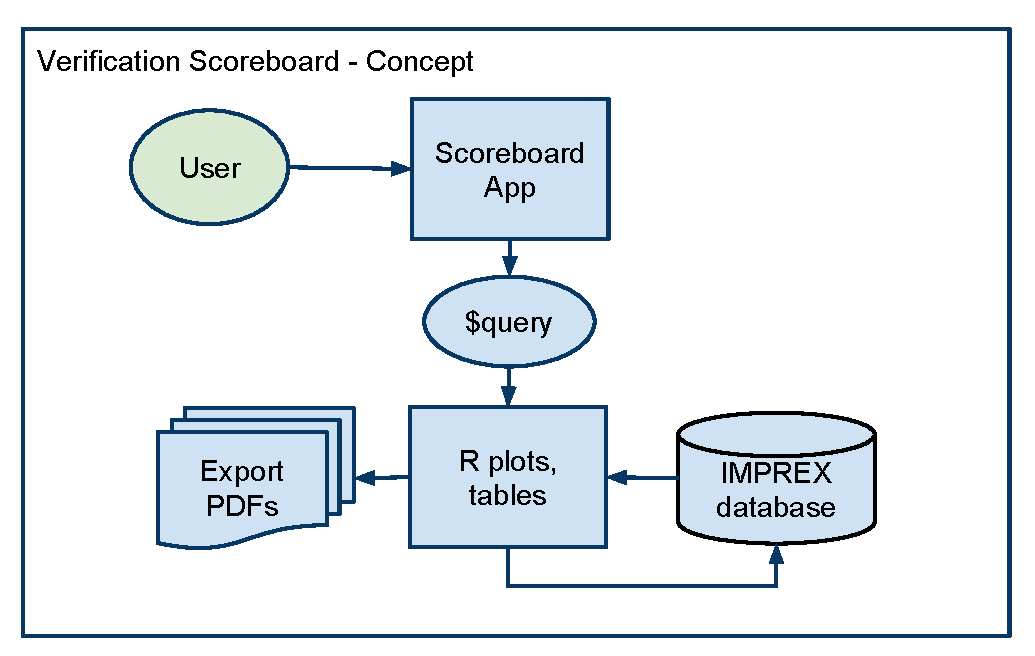
\includegraphics[width=0.85\linewidth]{images/IMPREX_Schema.pdf}
%{images/concept_verifscoreboard.png}
  \caption{Concept of a scoreboard.}
  \label{fig:scoreboard concept}
\end{figure}

Verification scoreboards are commonly used within a forecasting organization to validate their models and help tune future development efforts. 

\subsection{Investigation Questions}

This Masters dissertation project, and our contribution to the IMPREX project, seeks to create a shared back-end database with an open, customizable graphical user interface (GUI) to compare scores between forecast systems.

\subsection{Standardizing Data Input and Display}

Figure \ref{fig:scoreboard concept} shows a schematic view of the concept of scoreboard that we adopted in this study. A user opens the Scoreboard and start a query, which will allow the scoreboard to display plots and tables based on the score database maintained by the partners of the IMPREX project. All results may be exported as portable document format (PDF) files.

\gls{scoreboard-user} is the prospective consumer of the GUI. They interact with the visual component of the Scoreboard, the display; they also interact with the more complex component is the "plumbing", or interconnections, underneath.

In order for the scoreboard to display useful and interesting comparison data, users may upload their score data and explore individual or group plots, as well as compare against data other users have loaded. By definition, then, this shared database will be both receiving and displaying data, including standardizing data objects (model identifiers, time and date variables, etc) across models.

\gls{forecast-skill} is measured and displayed by the \gls{scoreboard-utility}.

The main challenges are:
\begin{itemize}
	\item Comparing comparable scores,
	\item Comparing comparable locations,
	\item Avoid misleading users.
\end{itemize}

In order to create a usable scoreboard we have created a web-based scoreboard which connects to a centralized database. To facilitate the introduction of this utility we have released the scoreboard as a stand-alone tool, which connects either to a locally-managed database or a series of flat files.

There is also the opportunity to install the Scoreboard on a web server, install the database, and connect them to make a high-performance web-based scoreboard. As the data we've used is considered "provisional", and appropriate servers have not yet been identified, this part of the concept is however not included in the work reported here.

\subsection{Some Limitations and Exceptions}

Forecast verification is a broad field. Over the course of the last few months I touched a tiny part of it, and here I enumerate some aspects of verification I omitted from this study:
\begin{enumerate}
	\item Spatial visualization of point (coordinate) data in Shiny: automatic data load for coordinates is hard (model systems may use custom coordinates, ex \gls{EFAS}) and layering in Shiny leaflet library slows the interface,
    \item Spatial correlation by shapefile (eg from a GIS): while R can do it, the PostgreSQL requires from extensions (PostGIS) which add complexity; also "expensive" to store shapefiles,
    \item We use score data calculated / loaded by IMPREX team members. Creating scores from raw paired prediction / observations (as is done in some verification systems) becomes too complex for this project's scope.
\end{enumerate}
% * <jeff@jnorville.com> 2016-09-09T09:07:18.456Z:
%
% Add other excluded material here from our numerous conversations
%
% ^.

%########################################################################
% First part - Forecast Verification
%########################################################################

\part{About Forecasts}

\section{Verifying Hydrometeorological Forecasts, an Overview}

Hydrological and meteorological forecast systems may be verified, checked for performance and quality, by running them on historical parameters -- where the answer is already defined. This is known as a hindcast or reforecast. The forecast systems can be run as if ``live'', that is to say using prior information only, to issue forecasts into the future. A medium-range system producing daily forecasts over the next month might have lead times from 0 (today) to 30.

Resulting datasets are comprised of predictions made on a date and extending to the forecast validity period. These are paired with observations made during the same time period.

The simplest verification might be to plot the two datasets on a timeline and give an eyeball-approximation of whether or not the forecast predicts the observations.
\begin{figure}[hb]
\centering
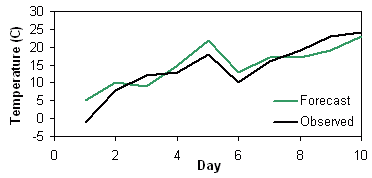
\includegraphics[width=0.45\linewidth]{images/eyeballtimeseries.png}
  \caption{Timeseries ``Eyeball'' Verification}
  \label{fig:eyeballSeries}
\end{figure}


Another type of visual verification could be performed on a map, the birds-eye view of a forecasted pattern with the observed weather at the time.
\begin{figure}[hb]
\centering
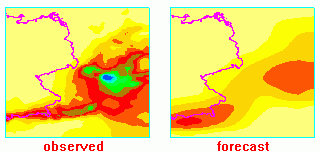
\includegraphics[width=0.45\linewidth]{images/DWDmaps.png}
  \caption{Spatial ``Eyeball'' Verification}
  \label{fig:eyeballMap}
\end{figure}

A more objective comparison may be made using numerical verification; this is simply a calculation done on the difference between the values, which typically degrade as lead time values increase.



\section{Motivation to Verify Forecasts}

Why verify a forecast? Numerical verification addresses administrative, scientific, and economic drivers. Before we get into that list, let me present a simple arithmetic question:

A bat and a ball cost €1.10. The bat costs €1 more than the ball. How much does the ball cost?

This example (borrowed from \textcite{kahneman2011thinking}) is often rapidly, intuitively answered as "ten cents", which is wrong - a simple check shows the trap: if the ball cost ten cents, the bat would be a euro more - €1.10 - giving a total of €1.20.

Intuitively, humans substitute an easier problem for a harder problem. It takes just enough effort to check our conclusion, to evaluate our "gut" response, that we often just don't do it.

Numerical verification -- checking the actual value, trends in scores -- is the kind of thing computers are particularly good at, and one reason we write so much software. The next sections of this thesis will address:
\begin{enumerate}
\item What is a verification score?
\item Which ones work, and why?
\item Different forecasts, different scores
\item Building our scoreboard
\end{enumerate}

\begin{figure}[hb]
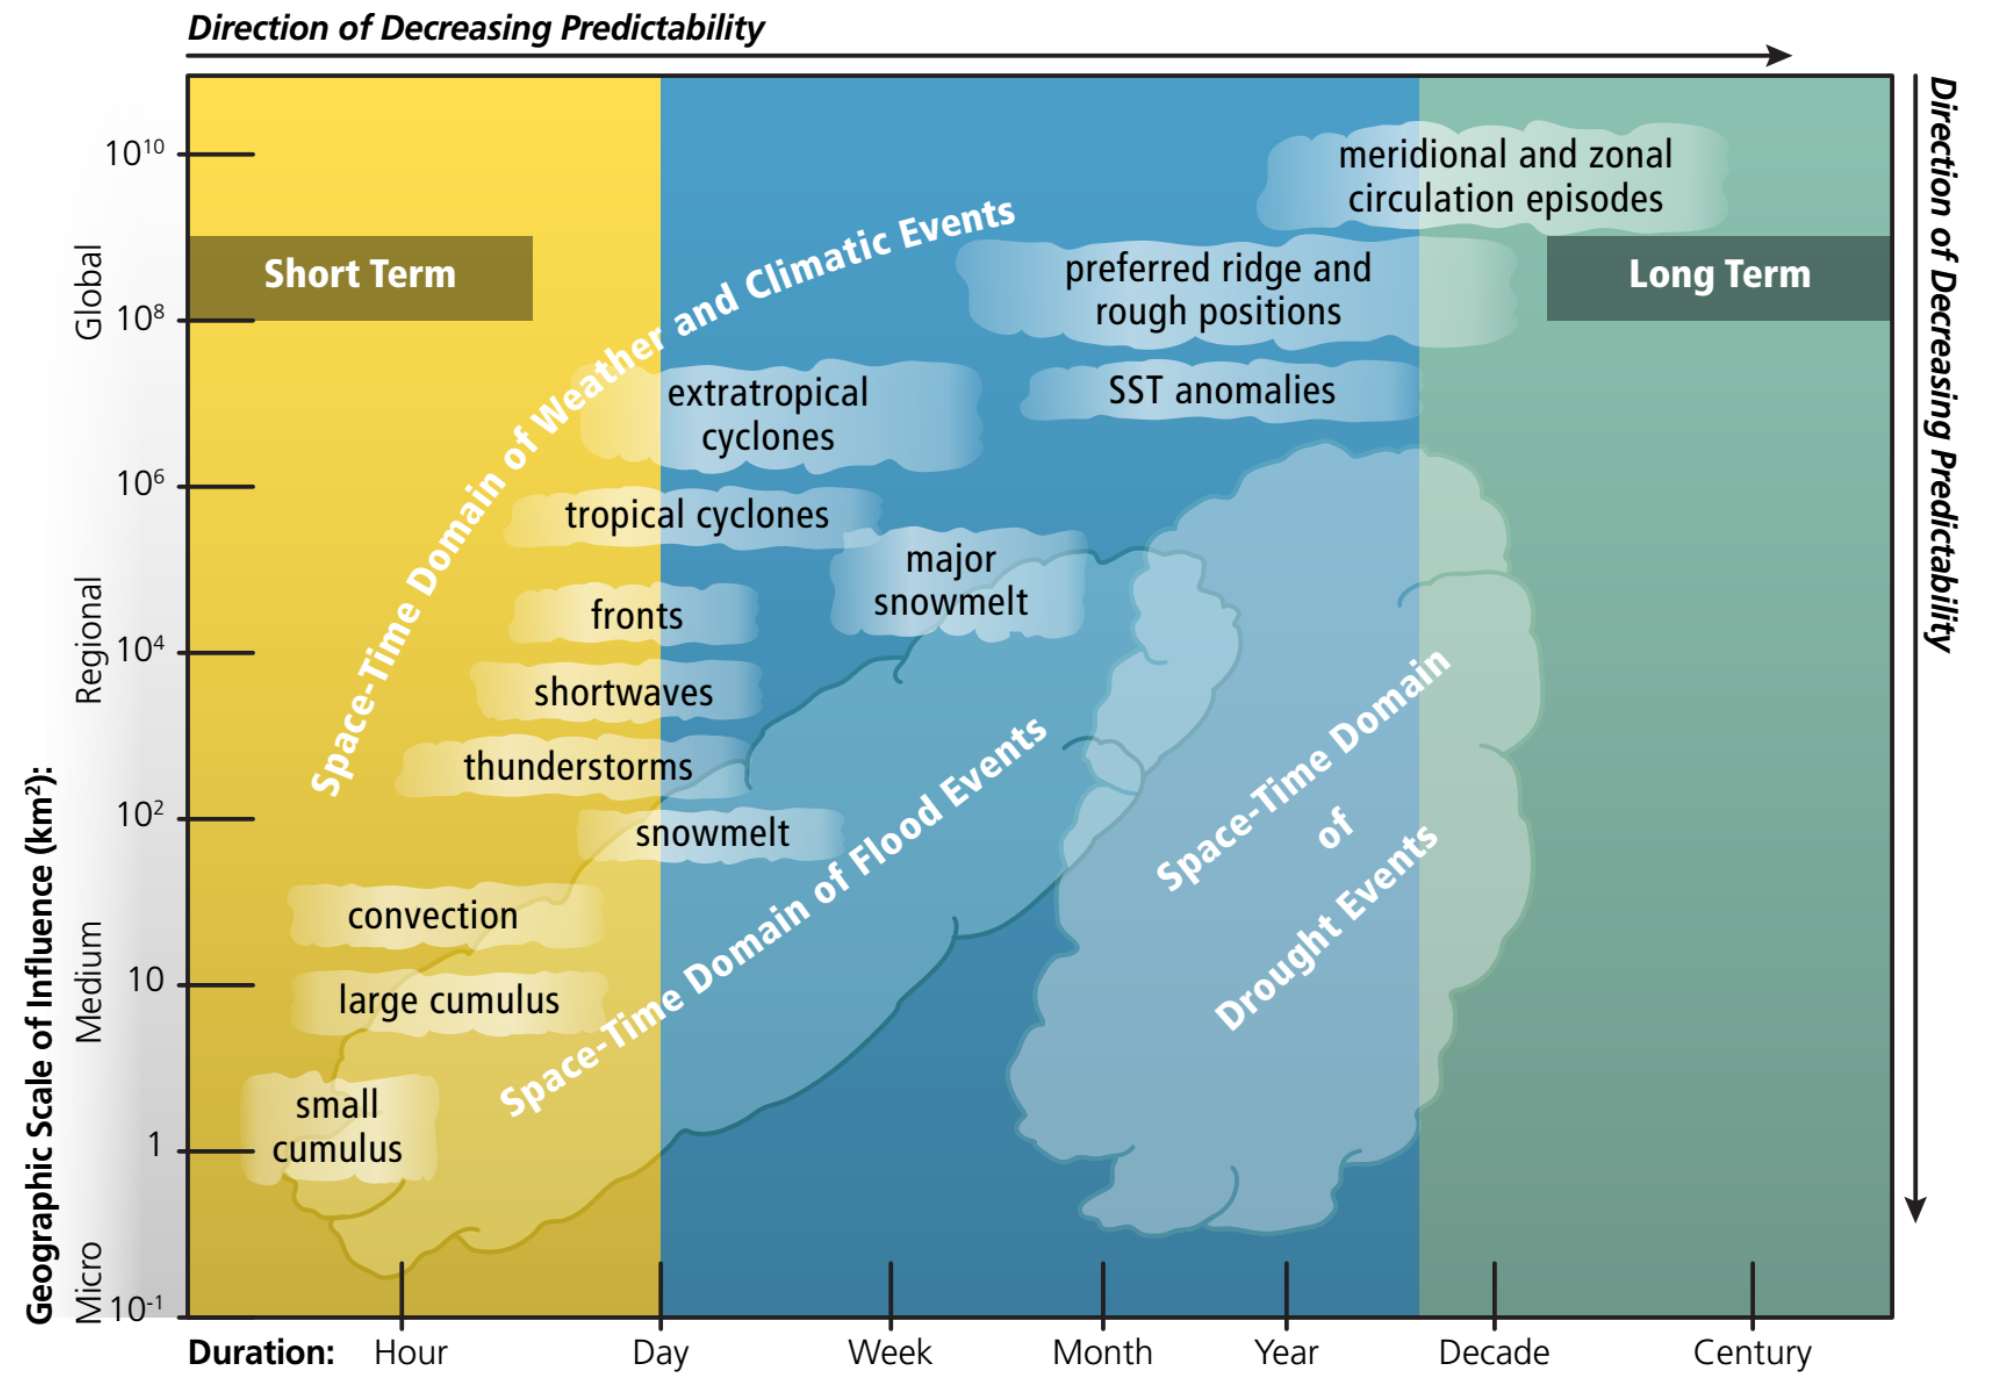
\includegraphics[width=\linewidth]{images/noaaSeasonalForecastProbs.png}
  \caption{Predictability and Forecast Event Type (SST: sea surface temperature) \autocite{jones2015cdwrproceedings}}
  \label{fig:noaa_seasonal_predictability}
\end{figure}

There are complicating factors in modeling and forecasting the physics of our planet. As Figure \ref{fig:noaa_seasonal_predictability} qualitatively illustrates, our ability to predict phenomena degrades with increasing scale (moving down the left axis), and moving from short term to long term forecasts (left to right). What is striking in this figure is the relative notion of meteorological events; flood, and drought events. The events that affect our societies and businesses aren't in the "easily-predicted" range.

\subsection{Administrative motivation}
Public agencies typically track their performance since they may be asked to justify funding requests, and it helps to quantify their gains over "competitors".

In "Forecast Verification" M. Jolliffe points out the UK Met Office offers "bounties" or rewards based on model performance quantified with internal scoreboard results. In practice, this can result in forecaster hedging.
\autocite{JolliffeIanT.andStephenson2012ForecastVerification}. 

A \gls{skill-score} is, as noted in the introduction, the quantitative identifier of prediction quality.

\subsection{Scientific motivation}

Finding errors or ill-conditioned components in a model, promoting or changing post-processing values, and/or noting when a change in a complex system had unintended influences are a few reasons scientists measure their model performance.

For Finley, he was simply overconfident in the value of his predictions; an objective verification process, or skill score comparison, would have probably highlighted to the interested observer that his predictive model wasn't worth promoting. 

Today, national weather centers share the results of their systems together; try to make comparisons of skill extended over different lead times; but it's difficult to agree on and to define a baseline for comparison.

\subsection{Economic motivation}

Different models may be conditioned for different answers. Consider the fictitious "northern latitudes" example from the introduction: the power company, interested in winter temperature fluctuations, while the highway sector waits on predictions of minimum temperature.

Models considered for use by the power company should be "scored" on their skill in predicting temperature fluctuations, or how well observations followed the model. On the other hand, the roadway authority would select the model with higher skill reported on detecting a specific temperature threshold.

In other sectors, a reservoir manager might be more interested in forecasts helping her understand peak demand for water usage from the reservoir. Disaster preparedness representatives for a downstream municipality would be interested in the forecast better-skilled at predicting the next flood.

These forecasts are generally conditioned on different data and variables, but a conversation about the models is outside the scope of this report. What is important is to understand that an objective skill score may be available for each sector, based on different data.

\section{Some Forecast Verification Scores}

% scores with examples from CAWCR :
%http://www.cawcr.gov.au/projects/verification/Finley/Finley_Tornados.html

Forecasters and practitioners often recommend using more than one score to better assess the attributes of a forecast such as reliability, resolution, discrimination and sharpness: “ any set of forecasts can then be ranked as best, second best, ...  worst, according to a chosen score, though the ranking need not be the same for different choices of score.”

Although verification scores themselves are typically run by the forecasting center generating the forecast, there are commonly agreed-on metrics in verification.

The CAWCR (Collaboration for Australian Weather and Climate Research) maintains a website \autocite{url:cawcr} describing many aspects and motivations to verify forecasts by a world-wide list of contributors, including a long list of well-known National Weather Centers and authors.

Some of the scores introduced on the CAWCR site are used in the scoreboard and database developed in this study, and introduced next: Skill scores, Brier score, RMSE, and CRPS.

\subsection{Skill Scores}

A skill score can be based on any of the following (Brier, CRPS, RMSE, etc) scores across different forecast systems, and is therefor one calculation we included in our Verification Scoreboard. 

The user specifies a fixed reference value for each forecast; then the score is calculated as a ratio of the different between each forecast and the reference value.

\begin{equation}
\label{eqn:SkillScoreEquation}
skillscore =  \frac{score_{forecast} - score_{reference} }{score_{perfect.forecast} - score_{reference}}
\end{equation}

As noted in the introduction, an early and classic forecast validation conversation was begun with the publication of Finley's tornadoes \autocite{murphy1996finley}. Here's a recreation of Finley's contingency table according to Murphy:

\begin{table}[H]
\centering
\begin{tabular}{lrccc}
\hline
 & \multicolumn{4}{c}{Observed} \\ \hline
\multicolumn{1}{l|}{} & \multicolumn{1}{l|}{} & \multicolumn{1}{c|}{tornado} & \multicolumn{1}{c|}{no tornado} & \multicolumn{1}{c|}{\textbf{total}} \\ \cline{2-5} 
\multicolumn{1}{l|}{} & \multicolumn{1}{r|}{tornado} & \multicolumn{1}{c|}{\cellcolor[HTML]{CBCEFB}28} & \multicolumn{1}{c|}{\cellcolor[HTML]{CBCEFB}72} & \multicolumn{1}{c|}{\cellcolor[HTML]{303498}{\color[HTML]{FFFFFF} \textbf{100}}} \\ \cline{2-5} 
\multicolumn{1}{l|}{} & \multicolumn{1}{r|}{no tornado} & \multicolumn{1}{c|}{\cellcolor[HTML]{CBCEFB}23} & \multicolumn{1}{c|}{\cellcolor[HTML]{CBCEFB}2680} & \multicolumn{1}{c|}{\cellcolor[HTML]{303498}{\color[HTML]{FFFFFF} \textbf{2703}}} \\ \cline{2-5} 
\multicolumn{1}{l|}{\multirow{-4}{*}{Forecast}} & \textbf{total} & \cellcolor[HTML]{303498}{\color[HTML]{FFFFFF} \textbf{51}} & \cellcolor[HTML]{303498}{\color[HTML]{FFFFFF} \textbf{2752}} & \cellcolor[HTML]{303498}{\color[HTML]{FFFFFF} \textbf{2803}} \\ \cline{2-5} 
\end{tabular}
\caption{Tornado Forecasts (1884 Finley)}
\label{tbl:TornadoForecasts}
\end{table}

As Finley argued, his forecasts were correct \((28 + 2680) / 2803 = 96.6\%\) of the time. However, if one assumed \textit{no tornado} -- an 'unskilful' forecast, or reference forecast -- the result is \(2752 / 2803 = 98.1\%\), an improvement on Finley's accuracy.

In calculating skill scores, different reference forecasts may be used. A common one is the average expected forecast, generally sampled at random over a large probabilistic forecast dataset to obtain a representative sample. The Finley example is a deterministic one, so the reference forecast is always "no forecast".

Other baselines used include "persistence", mostly used in short-term forecasts; this basically says "the weather this hour will be the same as the last hour". Skill greater than zero means the forecast predicted change when observed. Finally, "climatology" is a common reference used, where the mean value of the variable over time (ex 30 year period of observations) becomes the baseline. \autocite{JolliffeIanT.andStephenson2012ForecastVerification}

\subsection{RPS Score}

The Ranked Probability Score, a widely-used measure of probabilistic forecasts, is a squared quantification of the cumulative density function (CDF) of a forecast compared with the CDF of observations for the same / similar zone. 

This score is related to the Brier and CRPS scores, described below, and based on similar construction. A fundamental problem with the RPS, however, appears as bias when it's used on ensemble systems with smaller numbers of members (eg less than 40 \autocite{weigel2007discrete}).

\subsection{Brier Score, Brier Skill Score}

What's today called the Brier Score originally came from \autocite{brier1950verification}, called the \textit{sample skill score}, in one of the first probability forecast articles \autocite{Murphy1974ProbabilityForecasters}. In this paper Murphy and Winkler introduce Brier Score "calibration-refinement factors": reliability, resolution, and uncertainty.

The Brier score is popular because it's been collected for a long time; has been "updated" periodically \autocite{Murphy1974ProbabilityForecasters}; is straightforward to calculate (uses contingency tables); and is easy to interpret: if a Brier score is close to 0 it's close to perfect; the closer to 1 it gets, the worse it is.

%As in Table \ref{tbl:TornadoForecasts}, 
% * <jeff@jnorville.com> 2016-09-12T03:37:14.147Z:
%
% They highlight three likelihood-base-rate factors:
% 	\begin{enumerate}
%        \item Type-II conditional bias
%        \item discrimination, and
%        \item sharpness
%     \end {enumerate}
%
% ^.

\subsection{RMSE Score}

Also used in hydrogeological models, the Root Mean Squared Error is the square root of the mean of the squared differences between forecasts and observations.

The RMSE gives more weight on larger errors than smaller errors, which is advantageous if large errors are worse than small ones, A zero represents the perfect score.

% \subsection{Correlation}

% * <jeff@jnorville.com> 2016-09-09T12:09:58.637Z:
%
% \subsection{ROC score}
% The Relative Operating Characteristic (ROC) score 
% Relative Operating Characteristic, including the fitting of a smooth curve (bivariate normal model)
% ROC (Relative Operating Characteristic)
% Relative Operating Characteristic Score, including the integration of a fitted curve
% ROCS (Relative Operating Characteristic Score)
%
% ^.

% CRPS bias evaluated in ~\autocite{ferro2008effect}.

\subsection{CRPS score}

The CRPS (Continuous Ranked Probability Score) introduced in ~\autocite{hersbach2000decomposition} is a standard of verification metrics. It shared roots with the RPS, above, but is less influenced by spatial discritization of datapoints. It is one of the most-relied upon values and consistently appears in sample datasets we received.

As with other skill scores, the CRPSS (Continuous Ranked Probability Skill Score) is calculated using a reference score and a "new" score; a value of 0 is good, closer to 1 or -1 is not.

%########################################################################
% Tools and Workflow
%########################################################################

\part{Design of Scoreboard for Inter-Agency Comparison}

\section{Introduction} 

A challenge offered through this Masters dissertation was to create a scoreboard utility within the criteria of IMPREX project. The idea was to create a prototype and to test it with data sets generated by the group to evaluate both the function of the scoreboard.

Very little of the project was predefined. In the beginning a significant effort involved the selection of open-source software tools, an open workflow, and the "look and feel" of the scoreboard itself.

To accomplish these tasks I had to improve my knowledge and skills in a number of fields: understand verification of meteorological and hydrologic forecasts, learn the programming language R, evaluated file or database ``data warehouse'' options, and identify a platform that would also satisfy the goals of IMPREX.

\section{Requirements to Meet, Tools}

The technology for creating a web-based scoreboard which queries data from a database dates to the late 1990s; today such web-based systems are everywhere. What was unique about this project was finding the correct combination of tools to meet our requirements:
\begin{enumerate}
	\item Build an evaluation framework to benchmark the performance of hydrological forecasts
    \item Accommodate precipitation; temperature; flow discharge (with emphasis on discharges for my project)
    \item Prototype a (HTML) \textbf{user} interface for visualizing the scorecard, considering multiple choices
   	\item Prototype a \textbf{provider/user} interface for "feeding" the score database
	\item Should rely on Open Source tools
    \item Best to use tools familiar to IRSTEA team
    \item Should provide high-level programming environment
    \item Flexible enough to accommodate needs of the  (Europe-wide) IMPREX team
    \item Maintainable, readable code
    \item Test the scoreboard on seasonal reforecasts in France and at the global scale.
\end{enumerate}

Open Source software has a number of advantages over proprietary (closed) software: with many sets of eyes on the code, it often proves to be better thought-out and more robust. Open Source software is often distributed freely, and therefor may have a larger user base than a costly closed alternative. According to the appendix of "Forecast Verification" \autocite{JolliffeIanT.andStephenson2012ForecastVerification} written by Matthew Pocernich (National Center for Atmospheric Research in Boulder, Colorado, and author of much of the "verification" package in R), open source tools may be preferable for the research context: these tools often has a larger user base, increasing likelihood that errors will be discovered; the language with the larger user base  will likely be understood by more colleagues; and the source code may be evaluated and modified/extended if needed.
% * <jeff@jnorville.com> 2016-09-12T04:44:05.596Z:
%
% Closed or commercial software is generally more expensive that open source options, but may have more documentation, training, and support available. 
%
% ^.

After considering Python, Java, and Microsoft tools from Excel and Access to SqlServer, the environment at IRSTEA and the individuals I met at the Reading Weather Center seemed to share an enthusiasm for R (and either RStudio or Tinn-R).

To better assess the requirements and best tools for the development of the scoreboard utility, I met with hydrologists, meteorologists, infrastructure programmers, and others at ECMWA. They are experienced with the PostgreSQL database platform for storing and querying large data sets, and was impressed at the commitment to open source tools.

Eventually a suite of tools formed:

\begin{itemize}
\item R, from the \href{https://www.r-project.org/}{R project for Statistical Computing}
\item RStudio, the popular \gls{ide} from the eponymous \href{https://www.rstudio.com/}{RStudio} group
\item PostgreSQL, \href{https://www.postgresql.org/}{high-performance open source database}
\item Rmarkdown, an R package to create documents with R content by \href{https://www.rstudio.com/}{RStudio}
\item Shiny, an R package to create HTML5 web pages based on R content (also by \href{https://www.rstudio.com/}{RStudio})
\end{itemize}

Added to this list and discussed in the Workflow section, below, are the following tools which I used to write this document:

\begin{itemize}
\item git, an open source \href{https://git-scm.com/}{source control tool} which integrates nicely with RStudio
\item github, a \href{https://github.com/}{web-based git repository} which also functions as a backup
\item QGIS, the \href{http://www.qgis.org/fr/site/}{open source GIS platform} which I used to check locations and perform spatial queries
\item \gls{LaTeX}, text-based document preparation system
\item Overleaf, an online \href{https://www.overleaf.com/}{Document collaboration service} based on LaTeX
\item Mendeley, \href{https://www.mendeley.com/}{reference management system} like Endnote or JabRef, but integrates well with Overleaf
\end{itemize}

\section{Existing Scoreboards} \label{sec:ExistingScoreboards}

While there has not been a scoreboard designed to allow two climate centers to load their own score files, there are a number of different Scoreboards available today. Below are several examples: ECMWF based in Reading, UK; Met Office, based in the UK; NOAA, in the United States; and the KNMI Climate Explorer based in the Netherlands.

% examples
% http://www.wpc.ncep.noaa.gov/html/hpcverif.shtml
% http://apps.ecmwf.int/codes/grib/param-db
% MET:
% https://www.ral.ucar.edu/solutions/products/model-evaluation-tools-met
% http://www.dtcenter.org/met/users/

% * <jeff@jnorville.com> 2016-09-09T09:03:53.651Z:
%
% Inter-agency comparison missing from this otherwise thorough discussion about verification:
% http://staff.ucar.edu/browse/people/3623/OSGC-000-000-001-861
%
% ^.

\subsection*{NOAA Weather Prediction Center}
Some examples of scoreboards can be found from the websites of operational forecasting centers. For instance, Figure \ref{fig:noaaWPC} shows a screenshot of the webpage on verification statistics from the Weather Prediction Center of the National Weather Service of NOAA in US. The example shows the evolution of the Bias and the Threat scores over the period 1970-2015 for different lead times.

\begin{figure}[h]
\centering
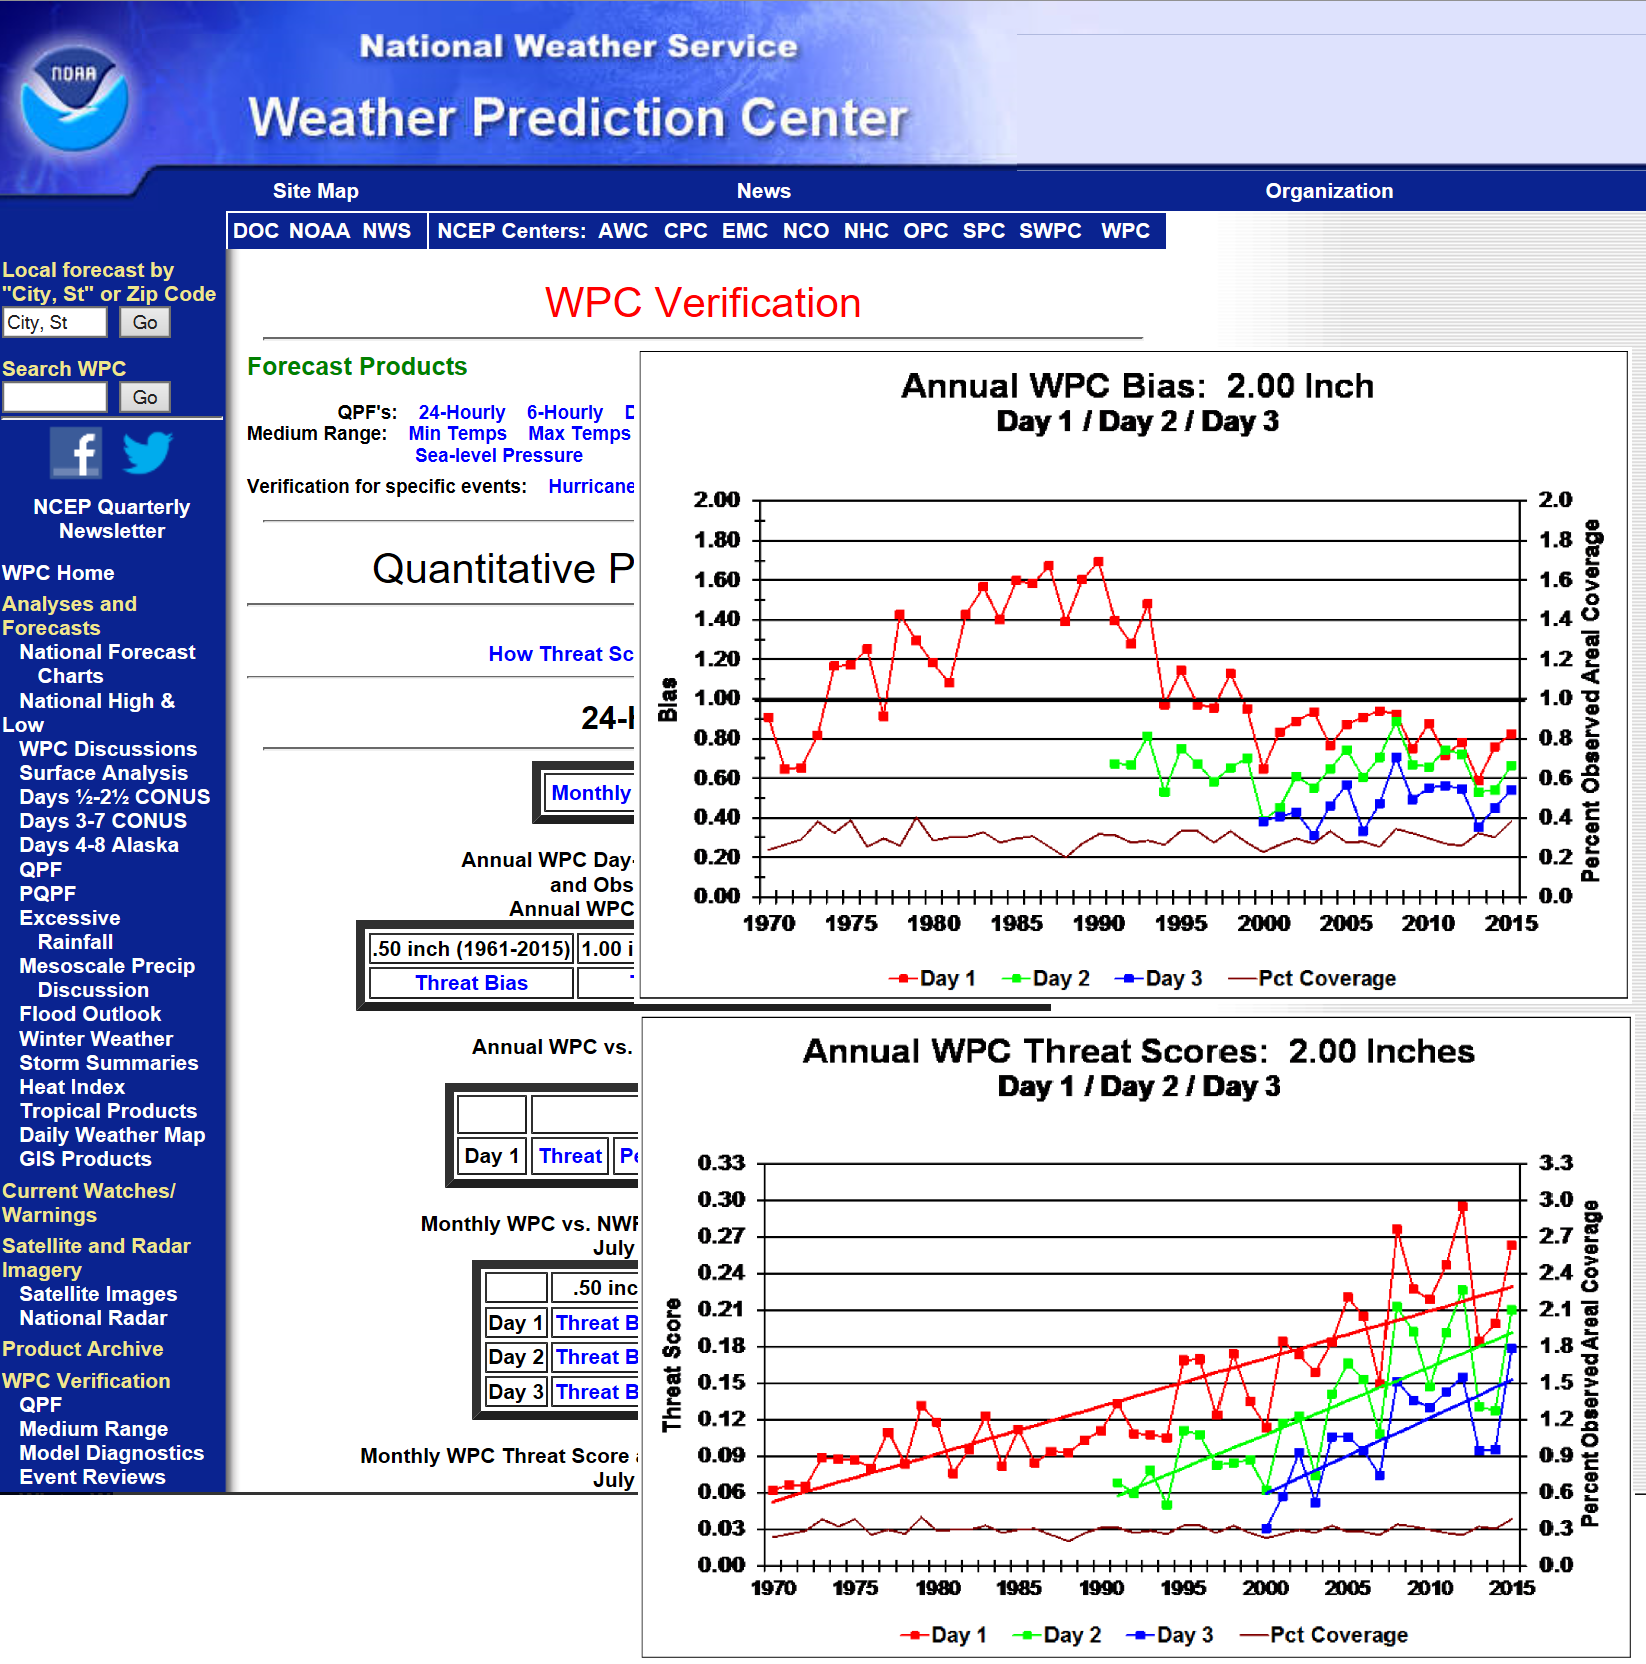
\includegraphics[width=0.85\linewidth]{images/exempleNOAAwpc.png}
  \caption{NOAA's Weather Prediction Center}
  \label{fig:noaaWPC}
\end{figure}

Also posted by NOAA, Figure \ref{fig:noaaSandy} shows the verification of Quantitative Precipitation Forecasts (QPF) provided for a single event: Hurricane Sandy, which affected most of the eastern United States (especially the coastal Mid-Atlantic States) autumn 2012. Verification is provided through the comparison of the maps of the accumulated precipitation forecasts and the accumulated observed precipitation over the affected areas.

\begin{figure}[H]
\centering
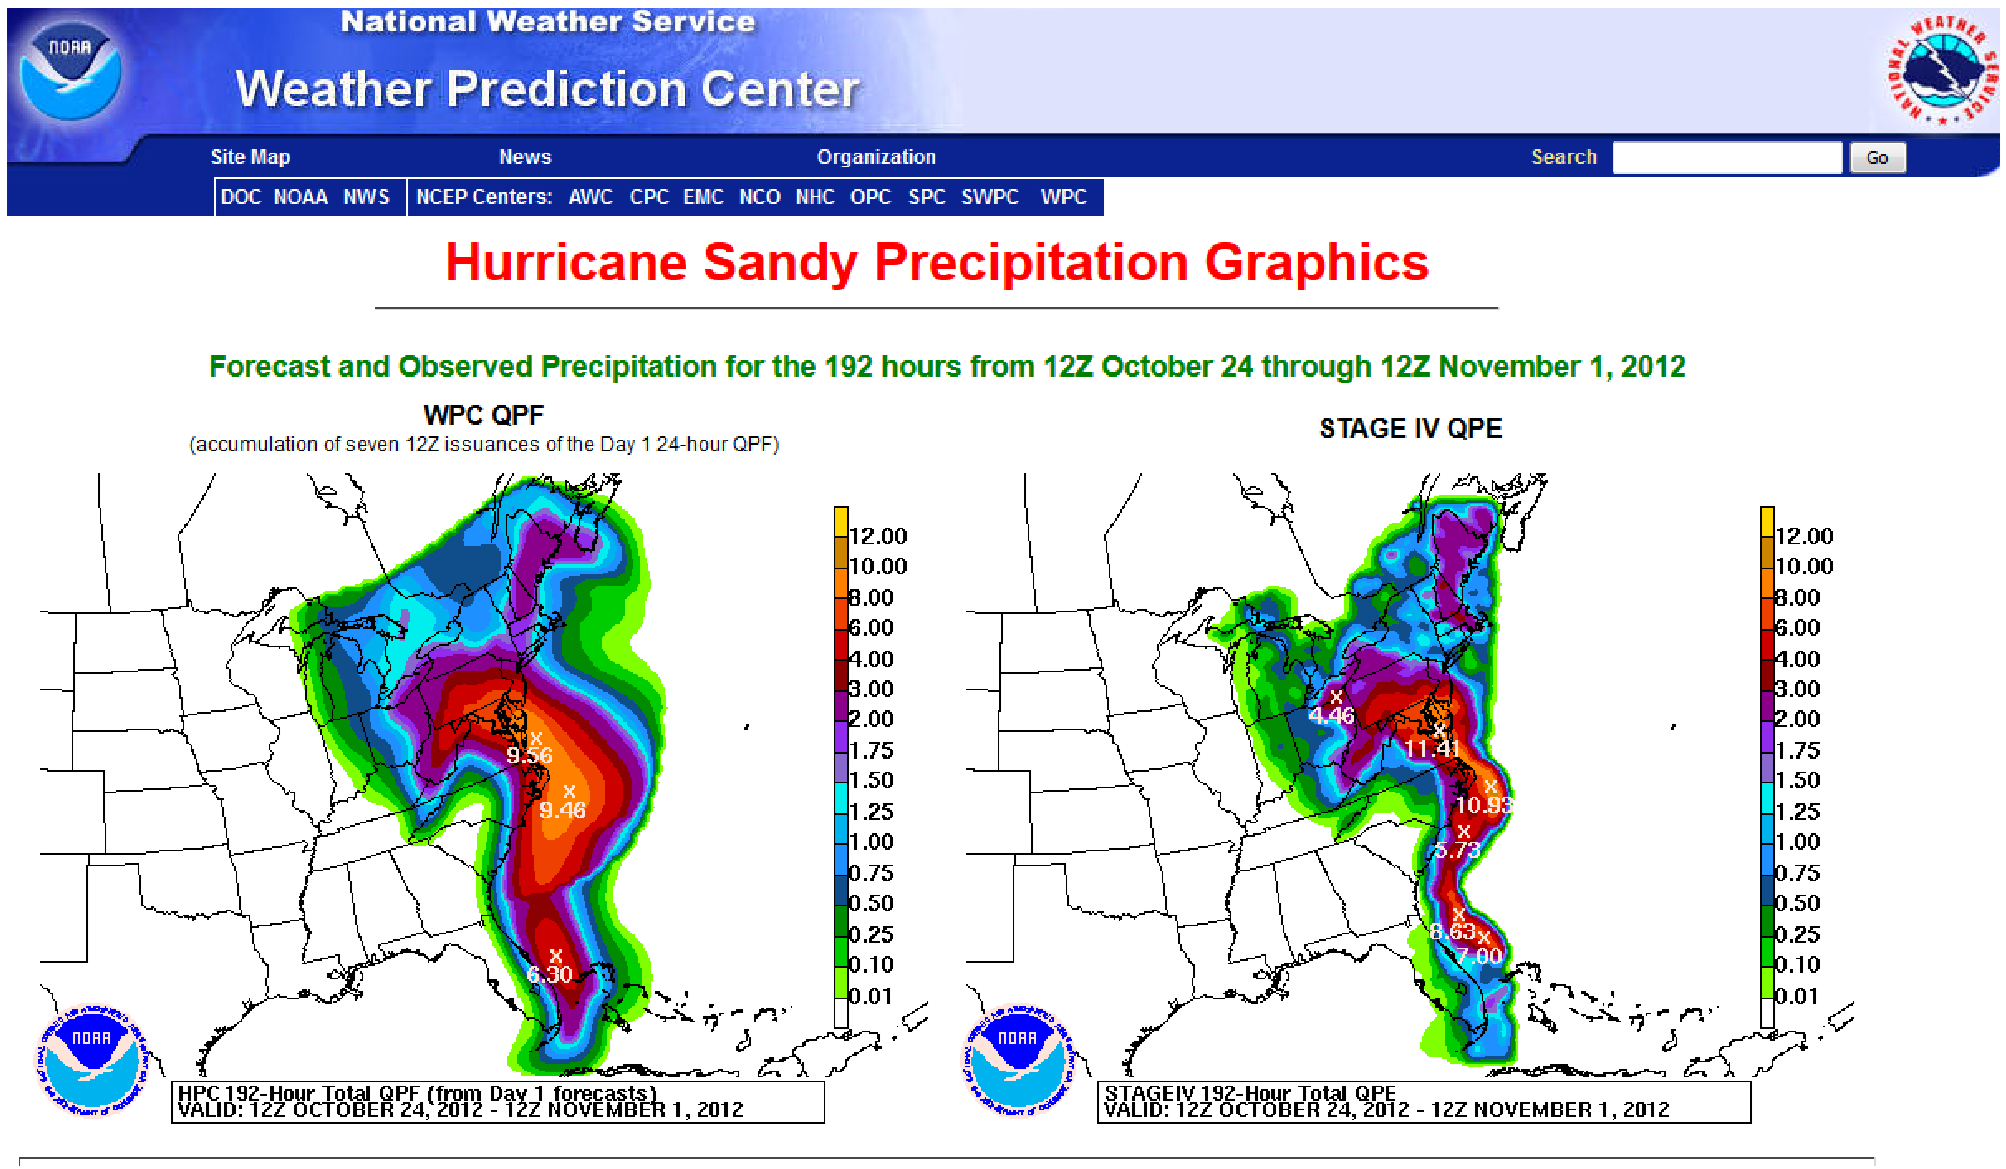
\includegraphics[width=0.70\linewidth]{images/noaaSandy.png}
  \caption{NOAA's Hurricane Sandy verification page}
  \label{fig:noaaSandy}
\end{figure}


NOAA's WPC Verification: \href{http://www.wpc.ncep.noaa.gov/html/hpcverif.shtml}{http://www.wpc.ncep.noaa.gov/html/hpcverif.shtml}

Link to \href{http://www.wpc.ncep.noaa.gov/tropical/case_studies/sandy_2012/sandyprecip.php}{NOAA Sandy Precipitation graphics}

\subsection*{ECMWF Verification and Charts}
The ECMWF has automated and opened to the public a number of verification tools; below the main page are three Brier Score plots for the same dataset over three lead times (4, 6 and 10 days). This nicely-illustrates the trade-off between skill and lead time.

\begin{figure}[hp]
\centering
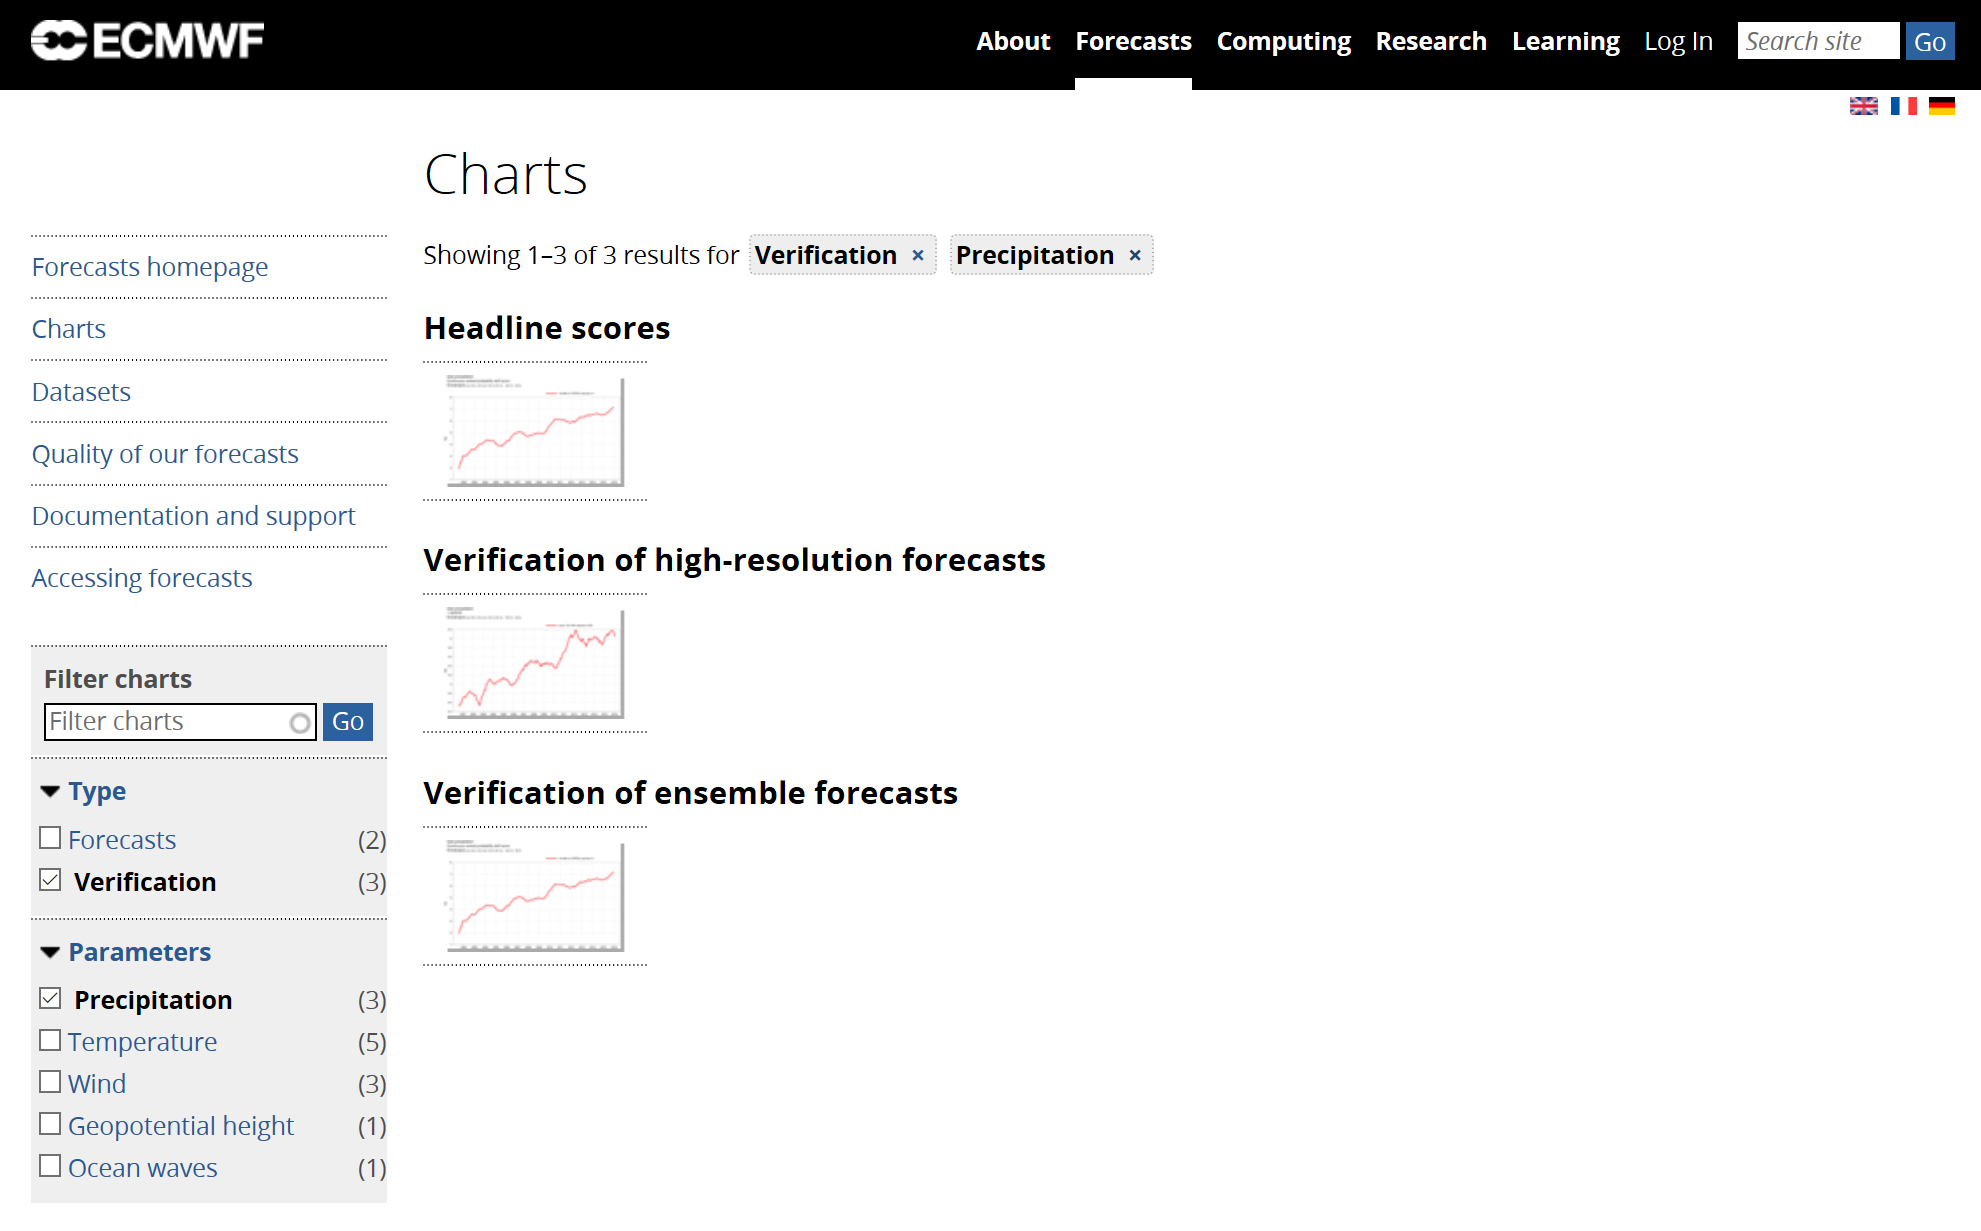
\includegraphics[width=0.7\linewidth]{images/exempleECMWFverifselect.png}
  \caption{ECMWF Forecast Verification Products}
  \label{fig:exECMWFverificationpage}
\end{figure}

\begin{figure}[hp]
\centering
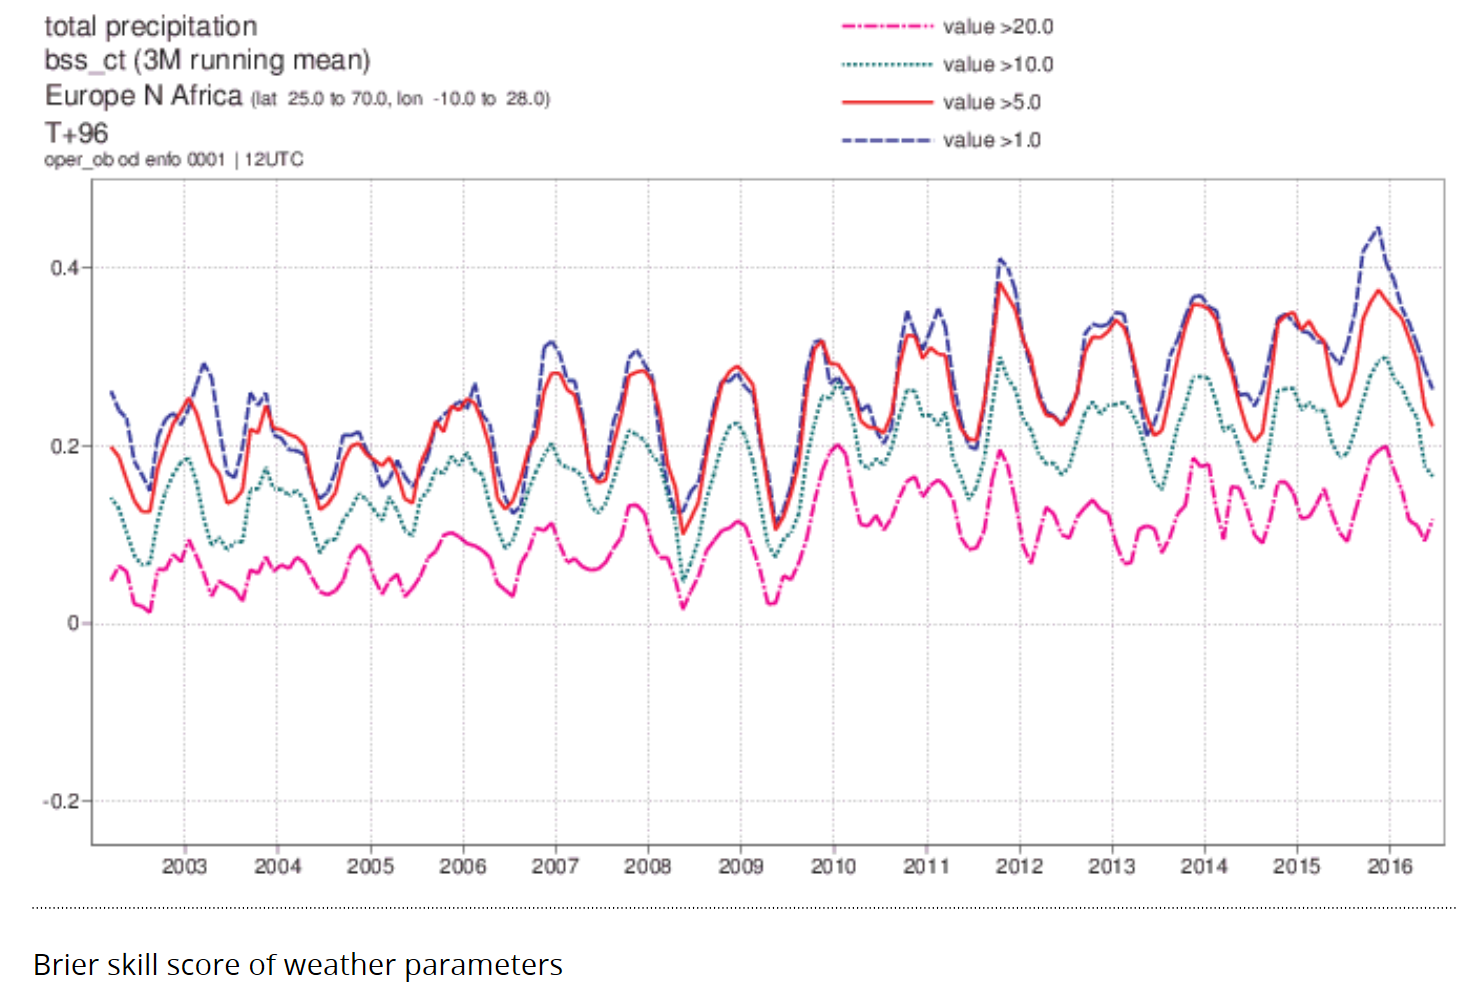
\includegraphics[width=0.6\linewidth]{images/exempleECMWF4day.png}
  \caption{ECMWF Brier Score on Precipitation; "forecast day" (lead time) = 4}
  \label{fig:ecmwfBrier4day}
\end{figure}

\begin{figure}[hp]
\centering
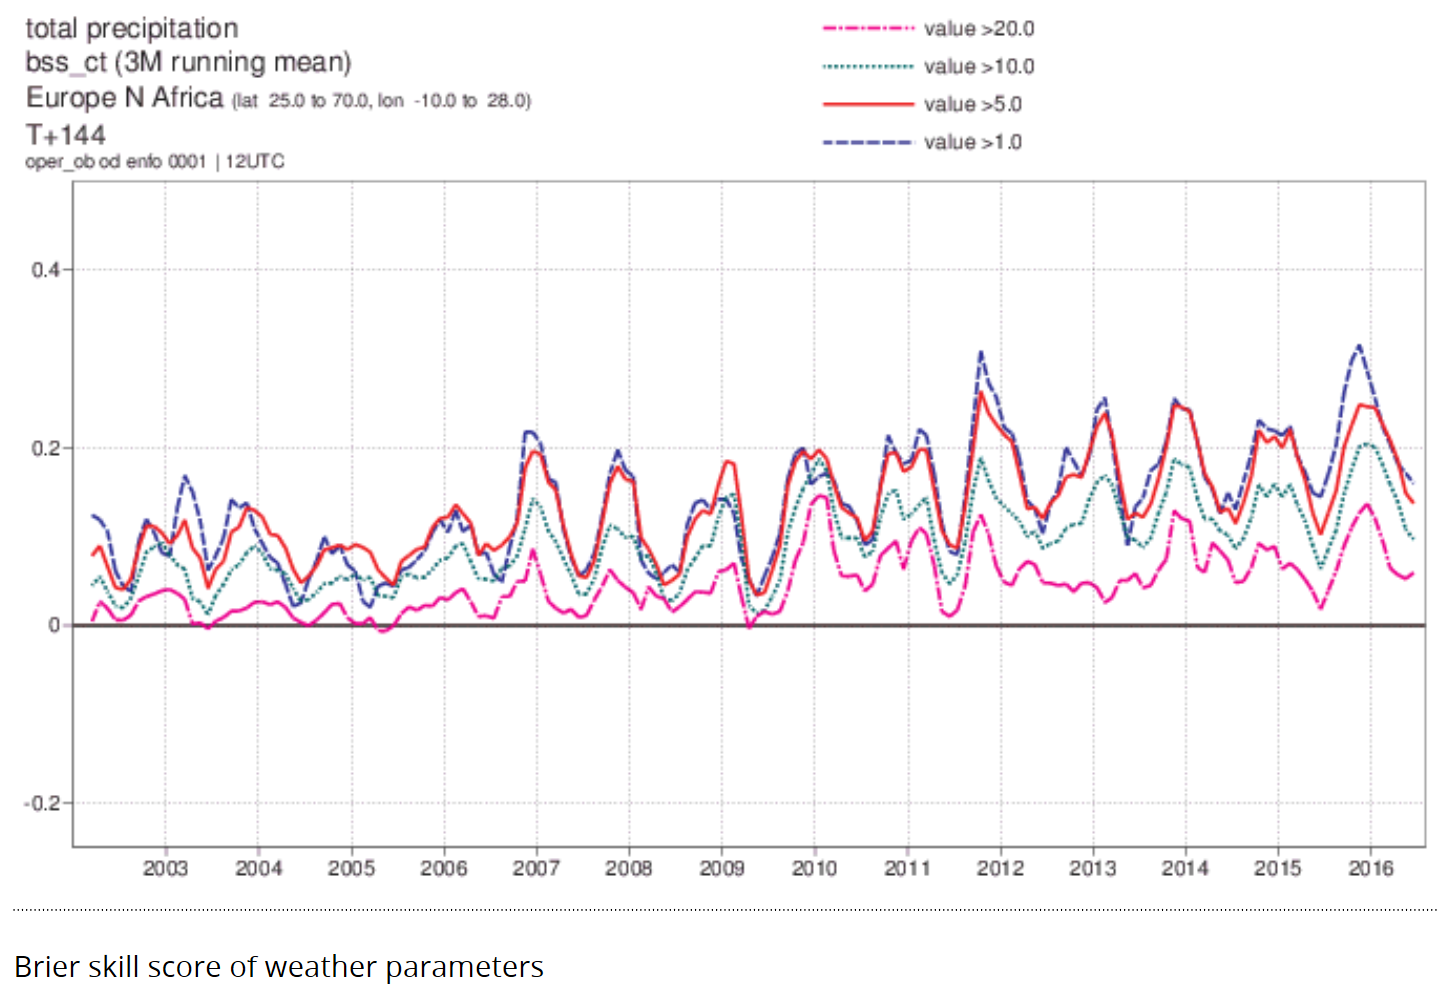
\includegraphics[width=0.6\linewidth]{images/exempleECMWF6day.png}
  \caption{ECMWF Brier Score on Precipitation; "forecast day" (lead time) = 6}
  \label{fig:ecmwfBrier6day}
\end{figure}

\begin{figure}[hp]
\centering
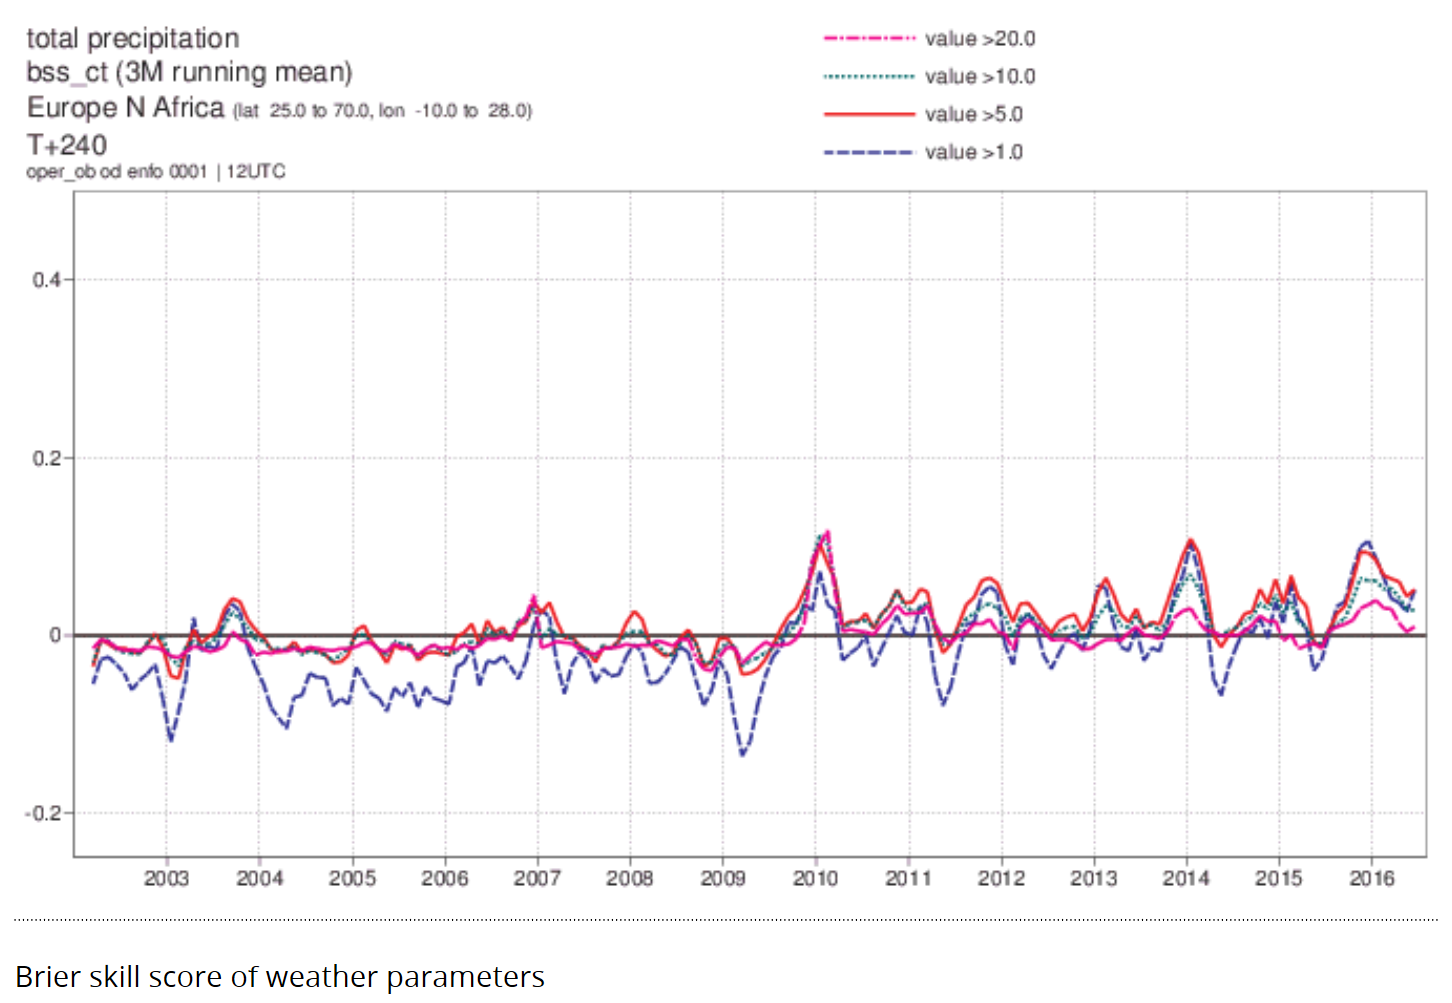
\includegraphics[width=0.6\linewidth]{images/exempleECMWF10day.png}
  \caption{ECMWF Brier Score on Precipitation; "forecast day" (lead time) = 10}
  \label{fig:ecmwfBrier10day}
\end{figure}

ECMWF's verification pages are here (select \emph{Type > Verification} to limit the page to verification products): \href{http://www.ecmwf.int/en/forecasts/charts/catalogue/}{http://www.ecmwf.int/en/forecasts/charts/catalogue/}



\subsection*{MetOffice}
Another example can be found in the website of the UK MetOffice for global long-range predictions. Probabilistic skill maps and plots are available and updated monthly for temperature and rainfall predictions up to six months ahead. Figure \ref{fig:metOffice1} illustrates how the user can change the “skill score type” to display a ROC score map or a Reliability diagram.

Other options on the visual display include the variable to display, the geographic area, and the period used for the computation of the scores.

The MetOffice webpage on global long-range model probability skill can be found here: \href{http://www.metoffice.gov.uk/research/climate/seasonal-to-decadal/gpc-outlooks/glob-seas-prob-skill}{http://www.metoffice.gov.uk/research/climate/seasonal-to-decadal/gpc-outlooks/glob-seas-prob-skill}

\begin{figure}[H]
\centering
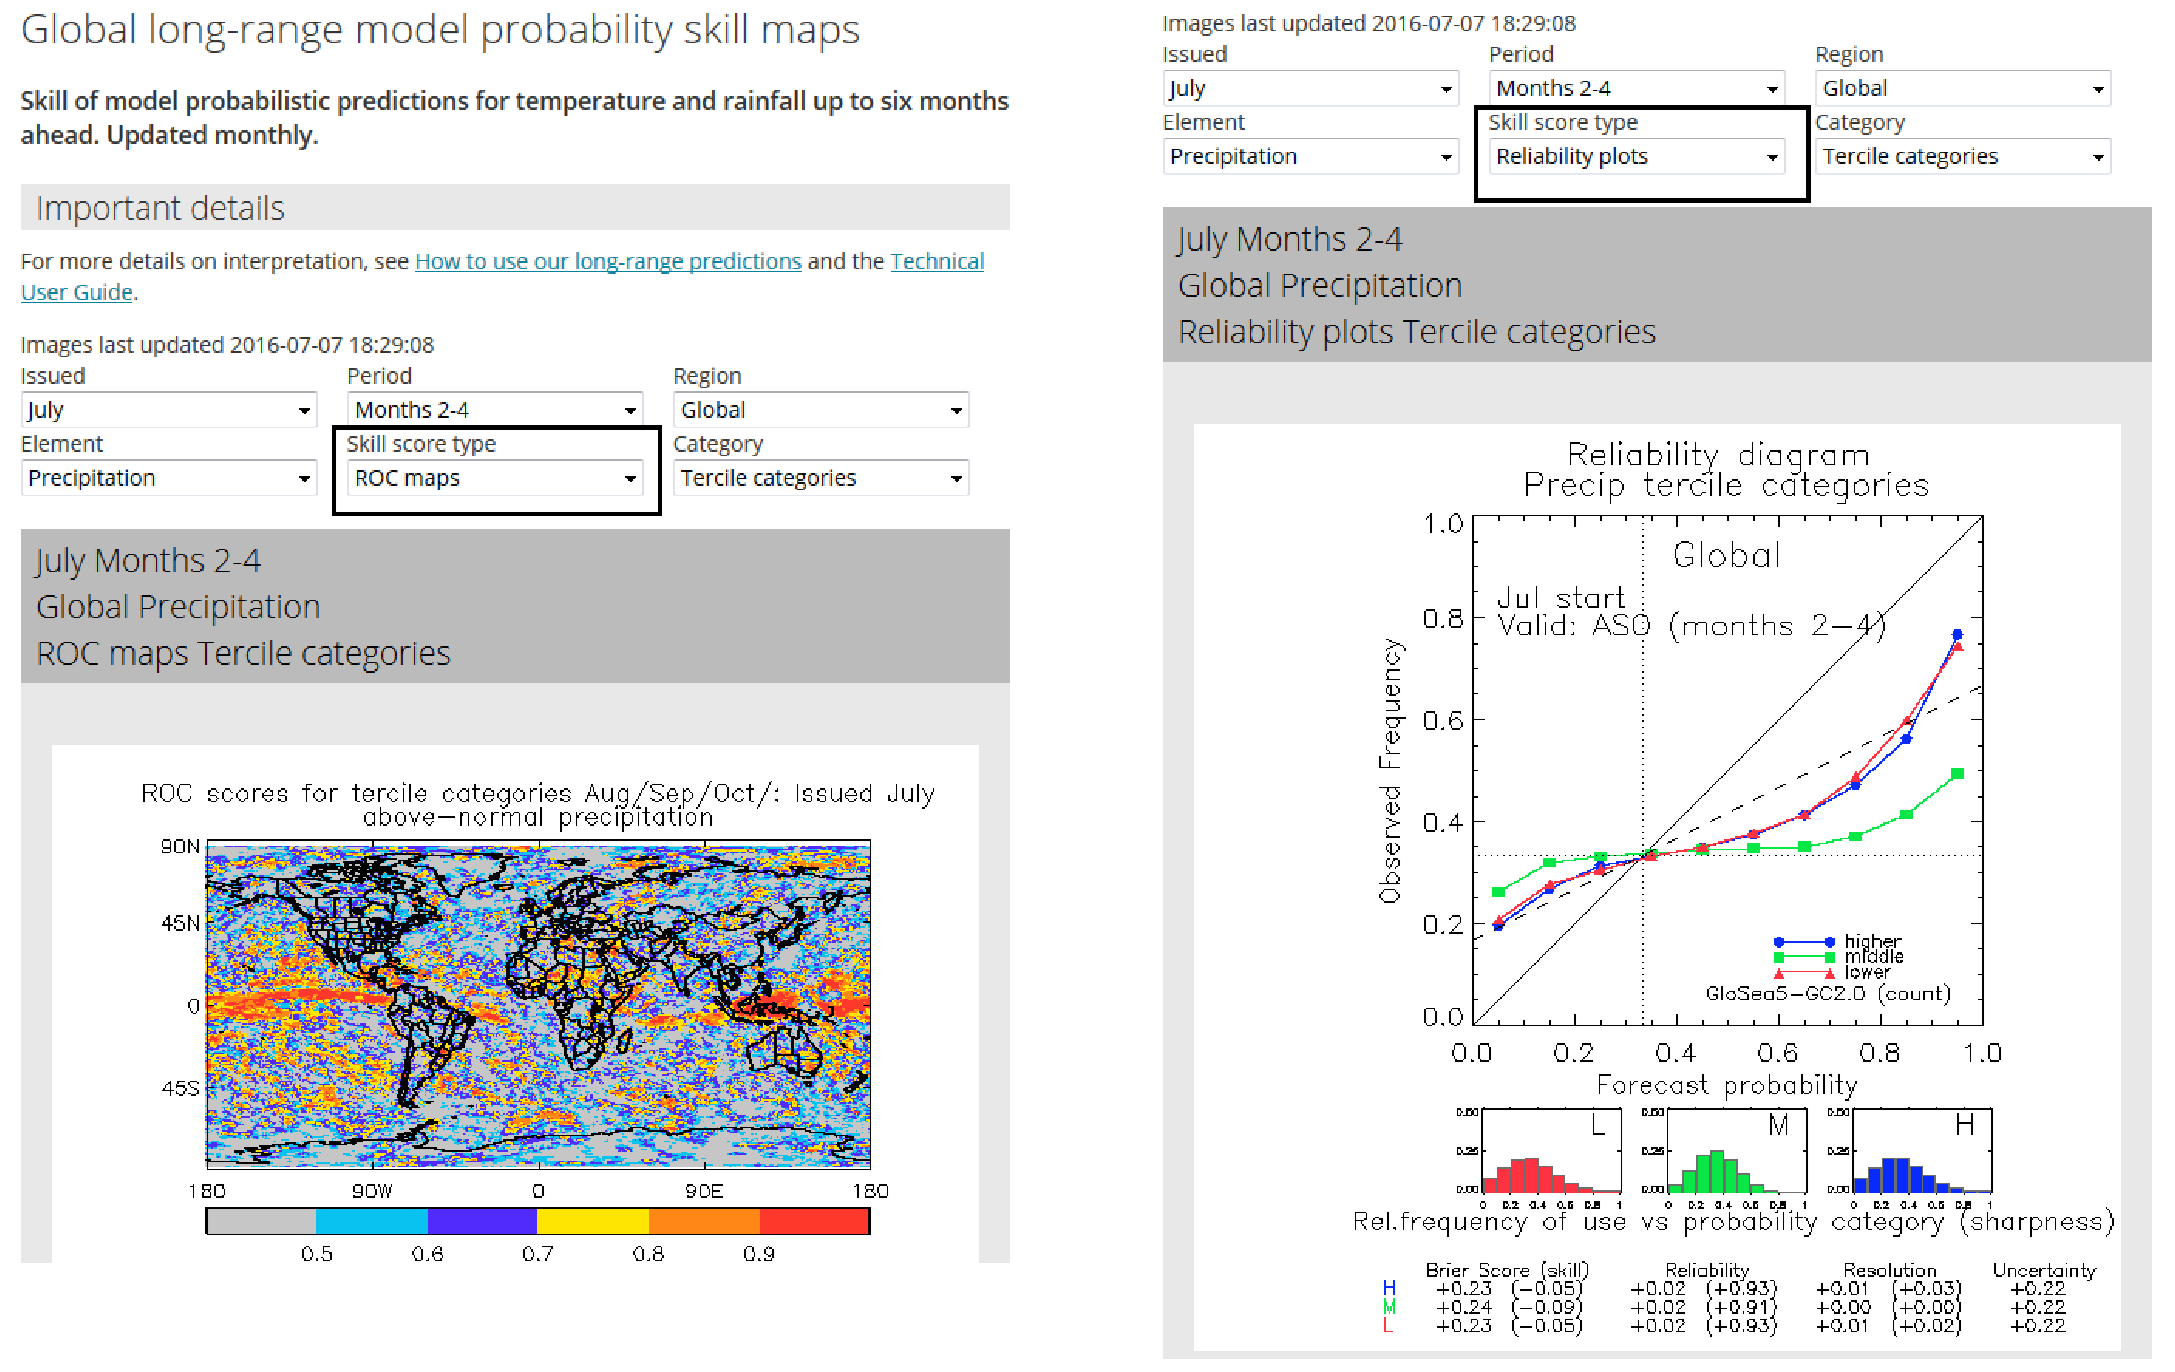
\includegraphics[width=0.80\linewidth]{images/exempleMetOffice1.png}
  \caption{MetOffice Prediction Center}
  \label{fig:metOffice1}
\end{figure}


\subsection*{KNMI Climate Explorer}
The KNMI Climate Explorer bridges the database of calculated forecasts, reforecasts and observations, and allows users to add their data. Data formats accepted include NetCDF and flat text files. Although we did not have access to that part of the site, it claims the capability to verify scores spatially (as in the NOAA Sandy page) as well as classically by time series over lead time.

\begin{figure}[hp]
\centering
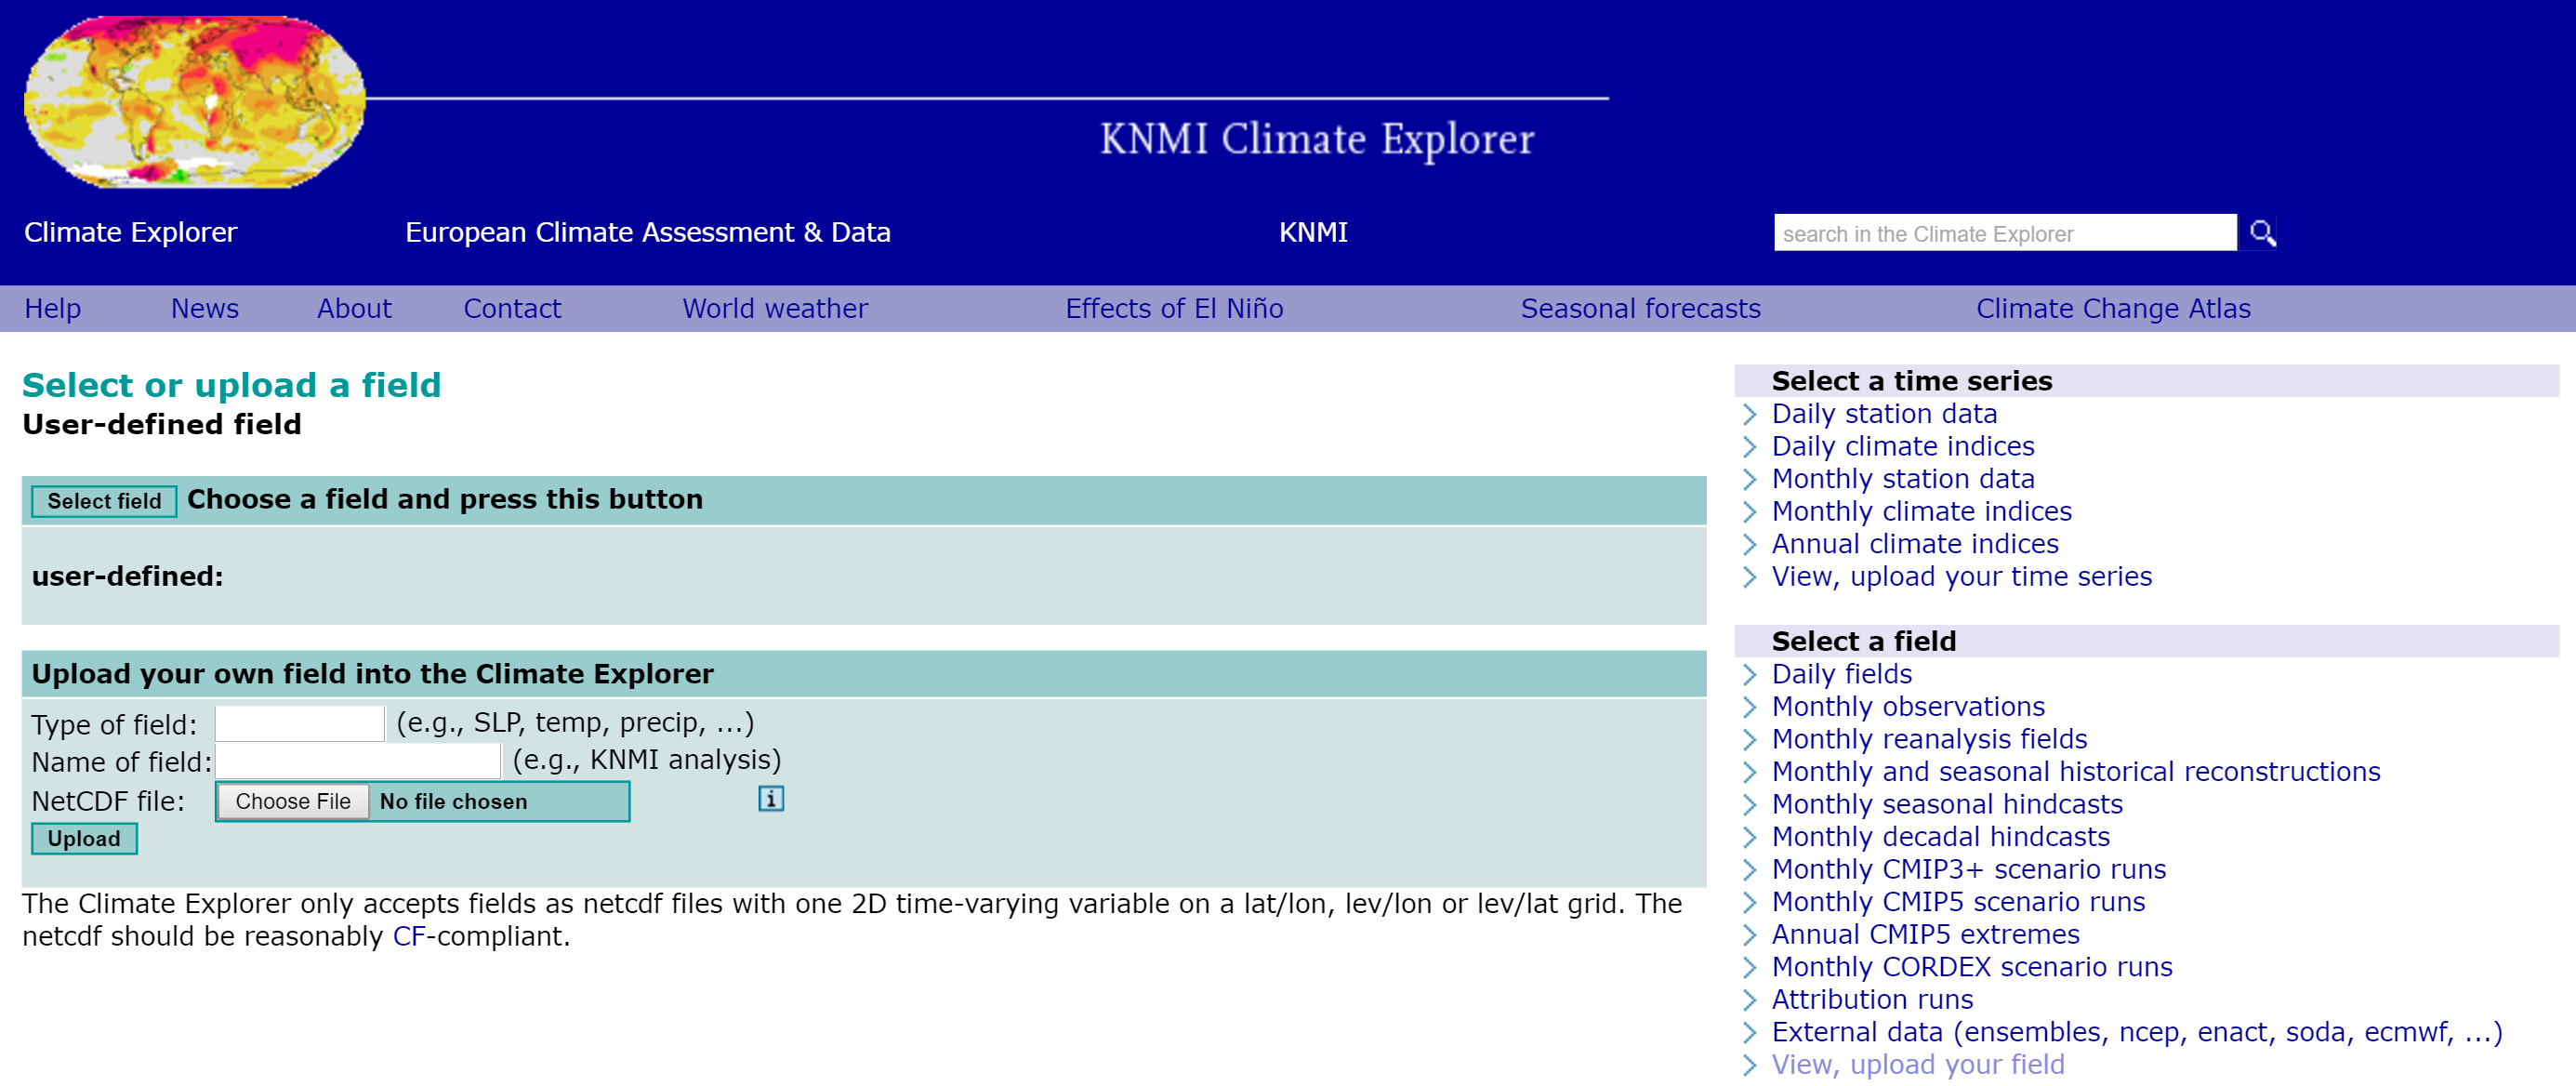
\includegraphics[width=0.70\linewidth]{images/vfsbKNMI1.png}
  \caption{KNMI's Climate Explorer works with internal forecast / observation files, or directly with NetCDF format}
  \label{fig:vfsbKNMI1}
\end{figure}

\begin{figure}[hp]
\centering
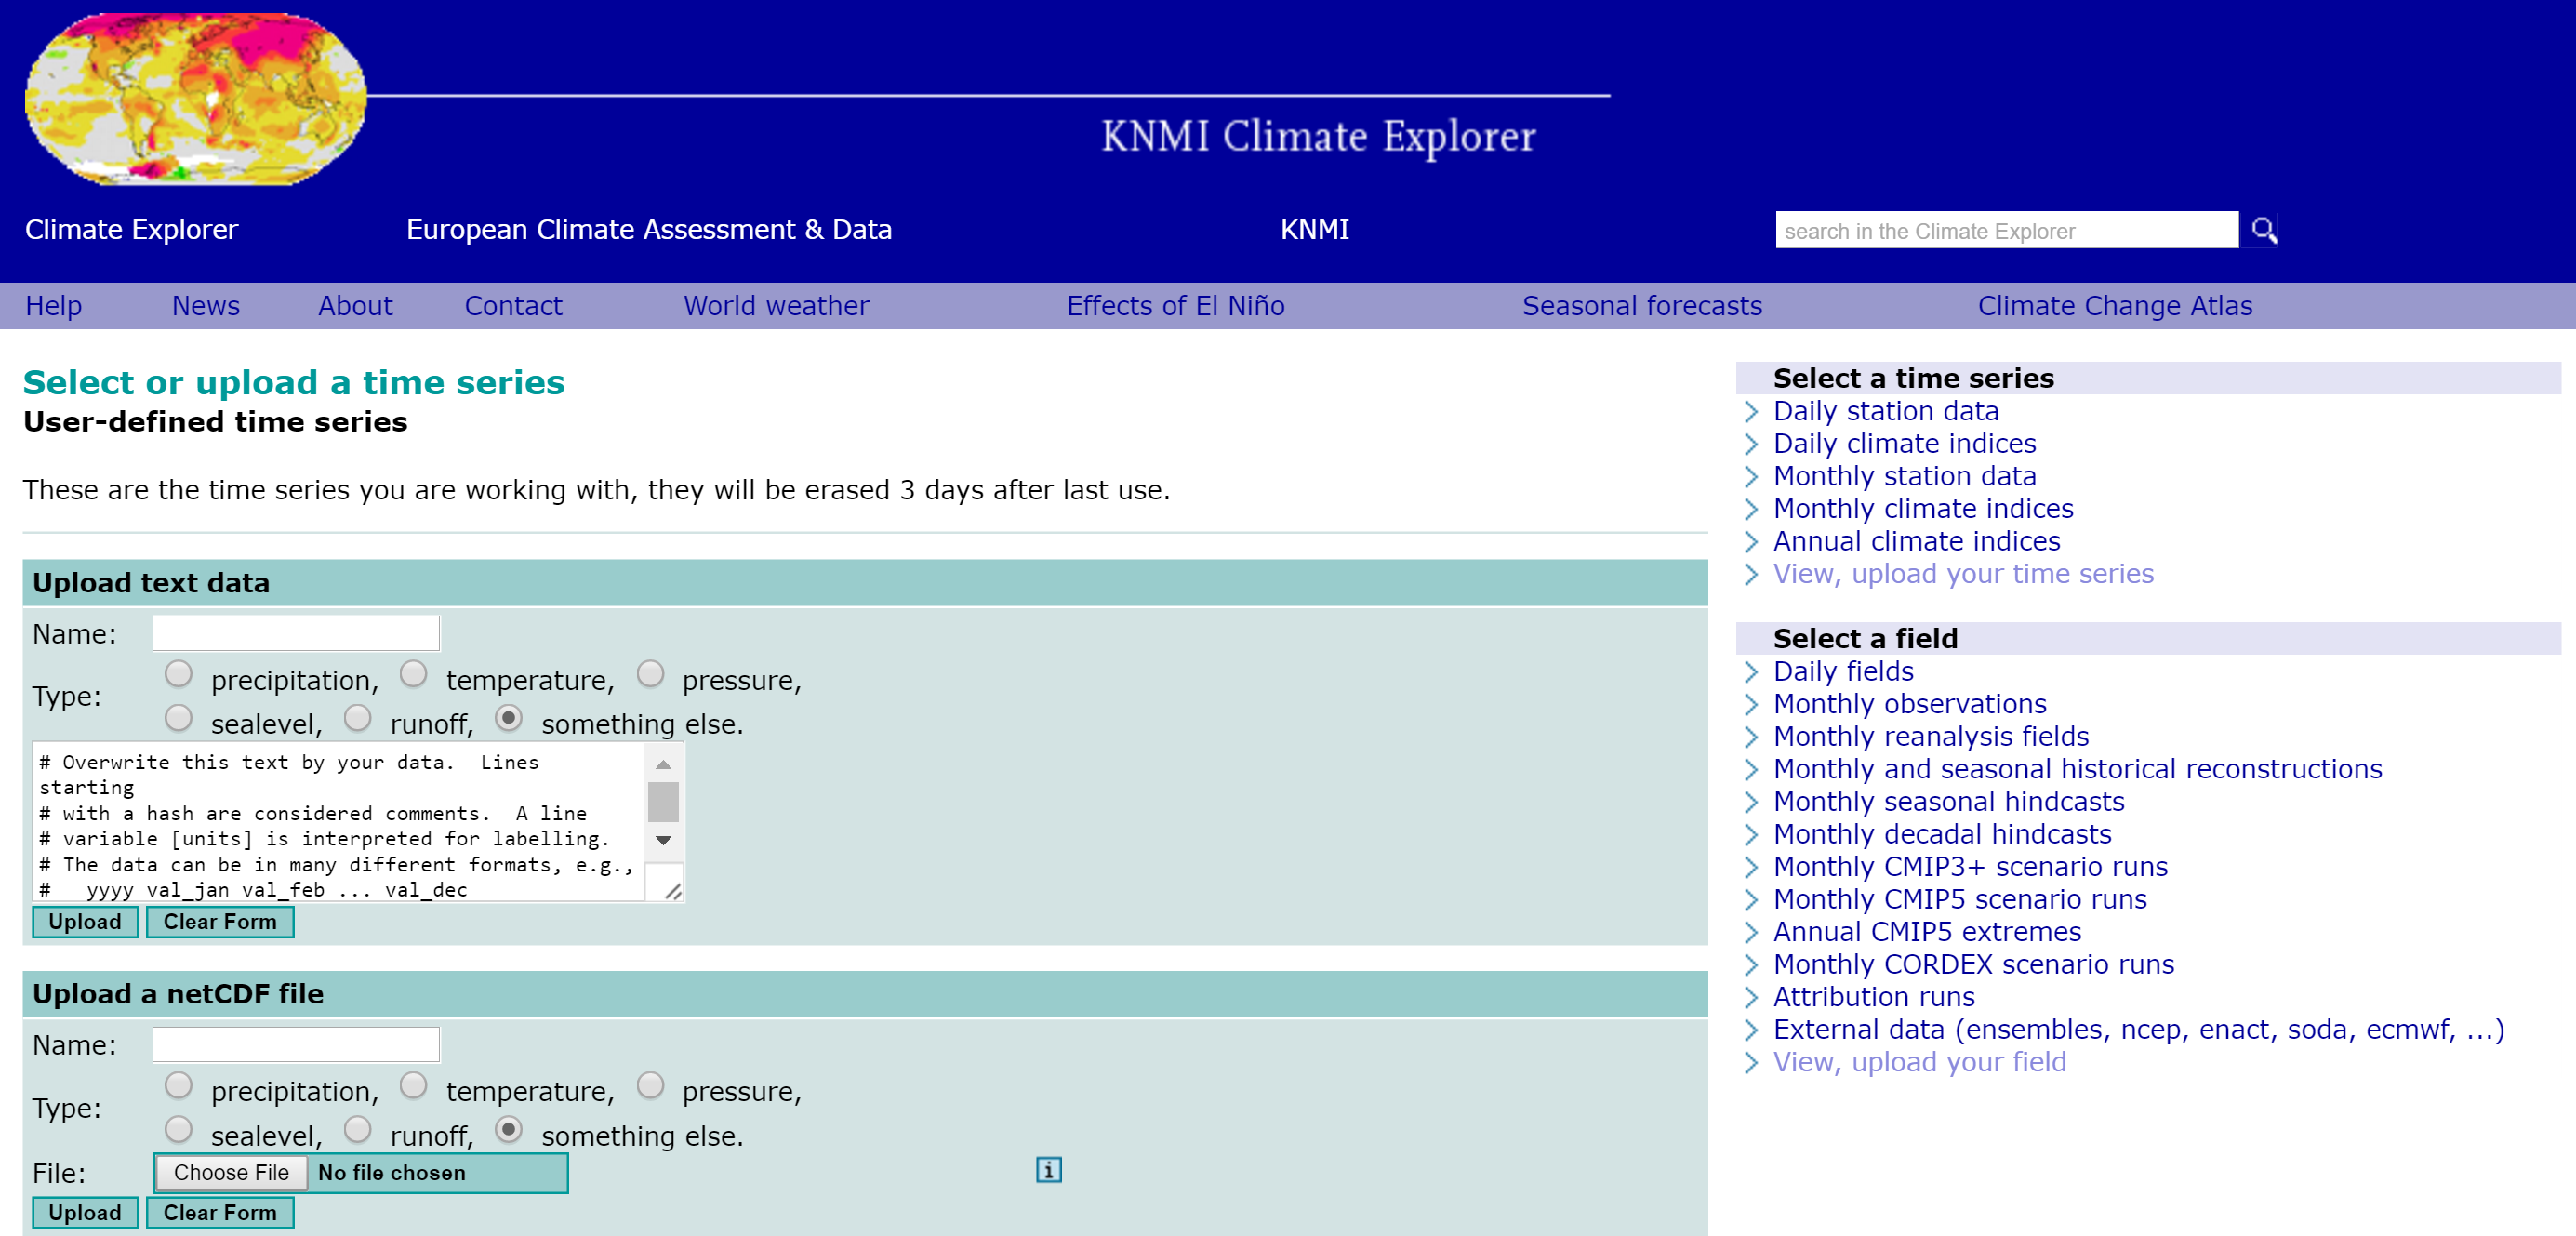
\includegraphics[width=0.70\linewidth]{images/vfsbKNMI2.png}
  \caption{KNMI's Climate Explorer allows users to upload their own text files}
  \label{fig:vfsbKNMI2}
\end{figure}

\begin{figure}[hp]
\centering
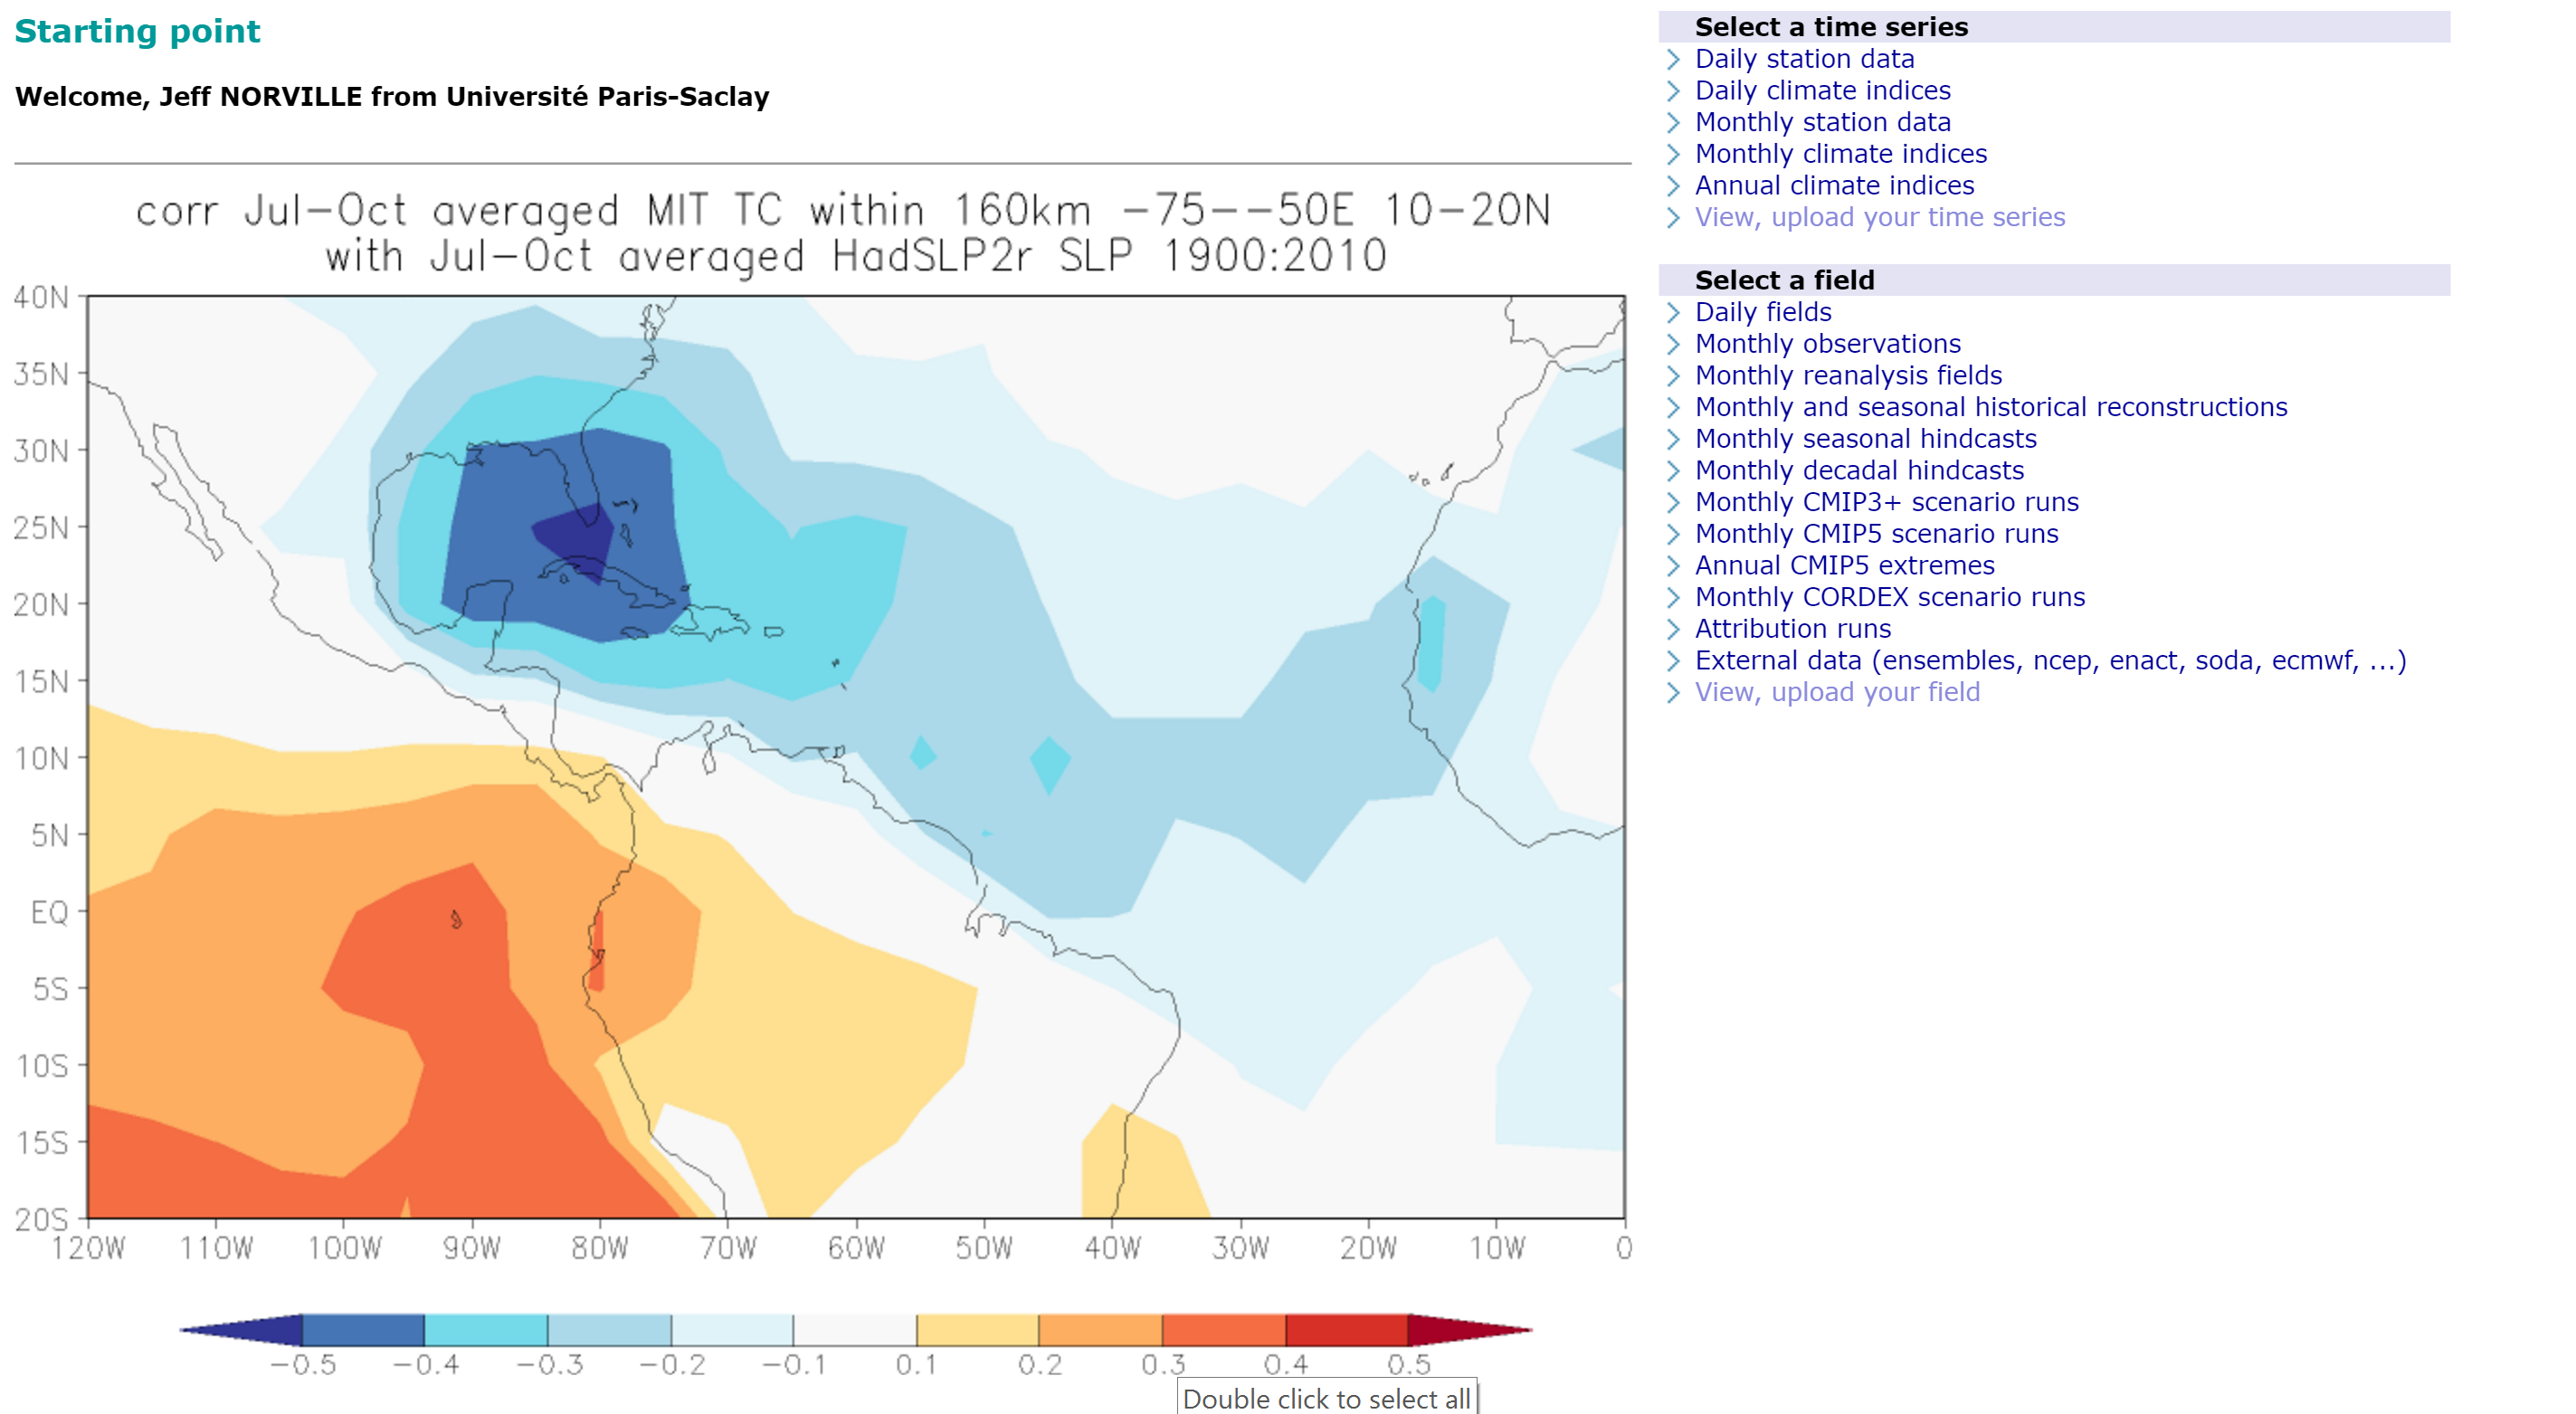
\includegraphics[width=0.70\linewidth]{images/vfsbKNMI3.png}
  \caption{KNMI's Climate Explorer with map-based verification. Note the page requires users to authenticate themselves}
  \label{fig:vfsbKNMI3}
\end{figure}

The KNMI Climate Explorer can be reached here; users need to sign in before proceeding the scores: \href{https://climexp.knmi.nl/}{https://climexp.knmi.nl/}




%########################################################################
%  Decisions made while developing the scoreboard
%########################################################################
\part{Technology Decisions: Workflow and Tools}

\section{Workflow}

While IRSTEA does use code standards, development source control systems, and team development standards for their Fortran and GR team development projects, this project involved non-statistical tools (Shiny package of RStudio, database and data manipulation suites of R libraries). However, as workflow is central to development and software lifecycle and improvements, we specify the processes below.

\subsection{Revision Control}

\begin{wrapfigure}{R}{0.25\textwidth}
\centering
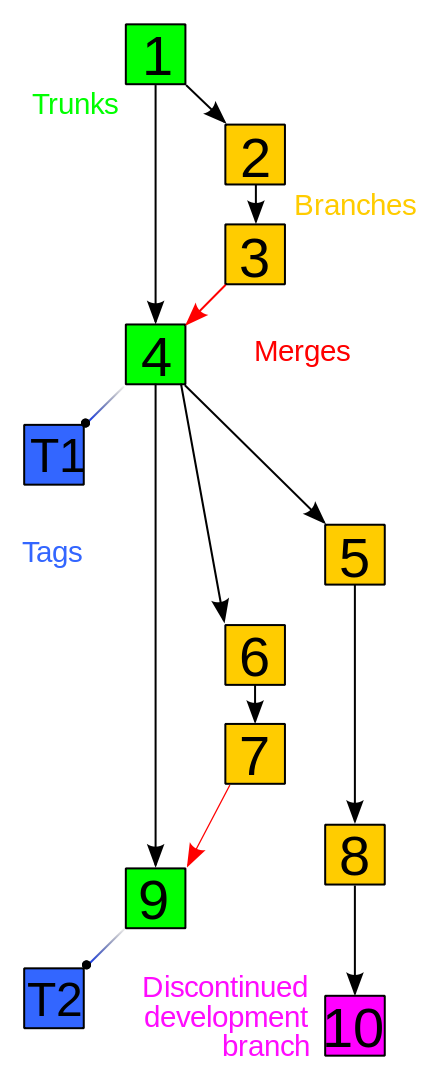
\includegraphics[width=0.22\textwidth]{images/440px-Revision_controlled_project_visualization-2010-24-02_svg.png}
  \caption{git Example Workflow}
  \label{fig:gitbranches}
\end{wrapfigure}

"\gls{source control}" or revision control is a way of tracking historical versions, changes from others, and testing new insights in an organized, systematic way. \textbf{git} and \textbf{github} are two system which support source control, but their similar names can be confusing. The program \textbf{git} (created by Linus Torvalds in 2005) is installed and runs on your local computer; it doesn't inherently need an internet connection, but creates a repository (or repo) locally. This means your first synchronization with a new git installation essentially recreates your added file(s) entirely; subsequent changes are stored only when you "commit" them to the repo.

The online service \textbf{github} doesn't require installation on your local computer, but, once signed up as a user (free), you can synchronize your local git repository with github and to see and share your source code online.

A critical concept in git and github is the "trunk" and "branch"; I include an introduction here, and refer the interested reader to more thorough and interactive documentation online: 
\href{https://guides.github.com/introduction/flow/}{https://guides.github.com/introduction/flow/}

The goal is to keep the "trunk" of the tree (usually called the master) as the always-clean, always-deploy-able code. When working on a new feature or fixing a bug, pull the latest code locally; create a well-named branch for your task (ex betterplots, below); improve code; commit it, and when it's ready to merge back into production there's any easy workflow below.

See Figure \ref{fig:gitbranches} for a visual scheme of a development trunk and individual branches. 

%\begin{minted}{tcsh}
%git pull #get the latest from repo trunk (Fig \ref{fig:gitbranches} 1)
%git checkout -b betterplots #checkout a new branch called betterplots (Fig \ref{fig:gitbranches} 2)
%# do work  (Fig \ref{fig:gitbranches} 3)
%commit #saving branch to repo
%git checkout master #move back to trunk
%git merge betterplots # merge betterplots to master trunk (Fig \ref{fig:gitbranches} 4)
%\end{minted}

The blue boxes in Figure \ref{fig:gitbranches} are "tags"; while similar to branches they are essentially dead-ends or archives, not living branches of the code repo.

For this project I started one github repo (\href{https://github.com/jeffnorville/shinysb1/}{https://github.com/jeffnorville/shinysb1/}) in April (Figure \ref{fig:githubactivity}), then moved to a "cleaner" repo for the deployable project: (\href{https://github.com/jeffnorville/VerifScoreboard}{https://github.com/jeffnorville/VerifScoreboard})

\begin{figure}[H]
\centering
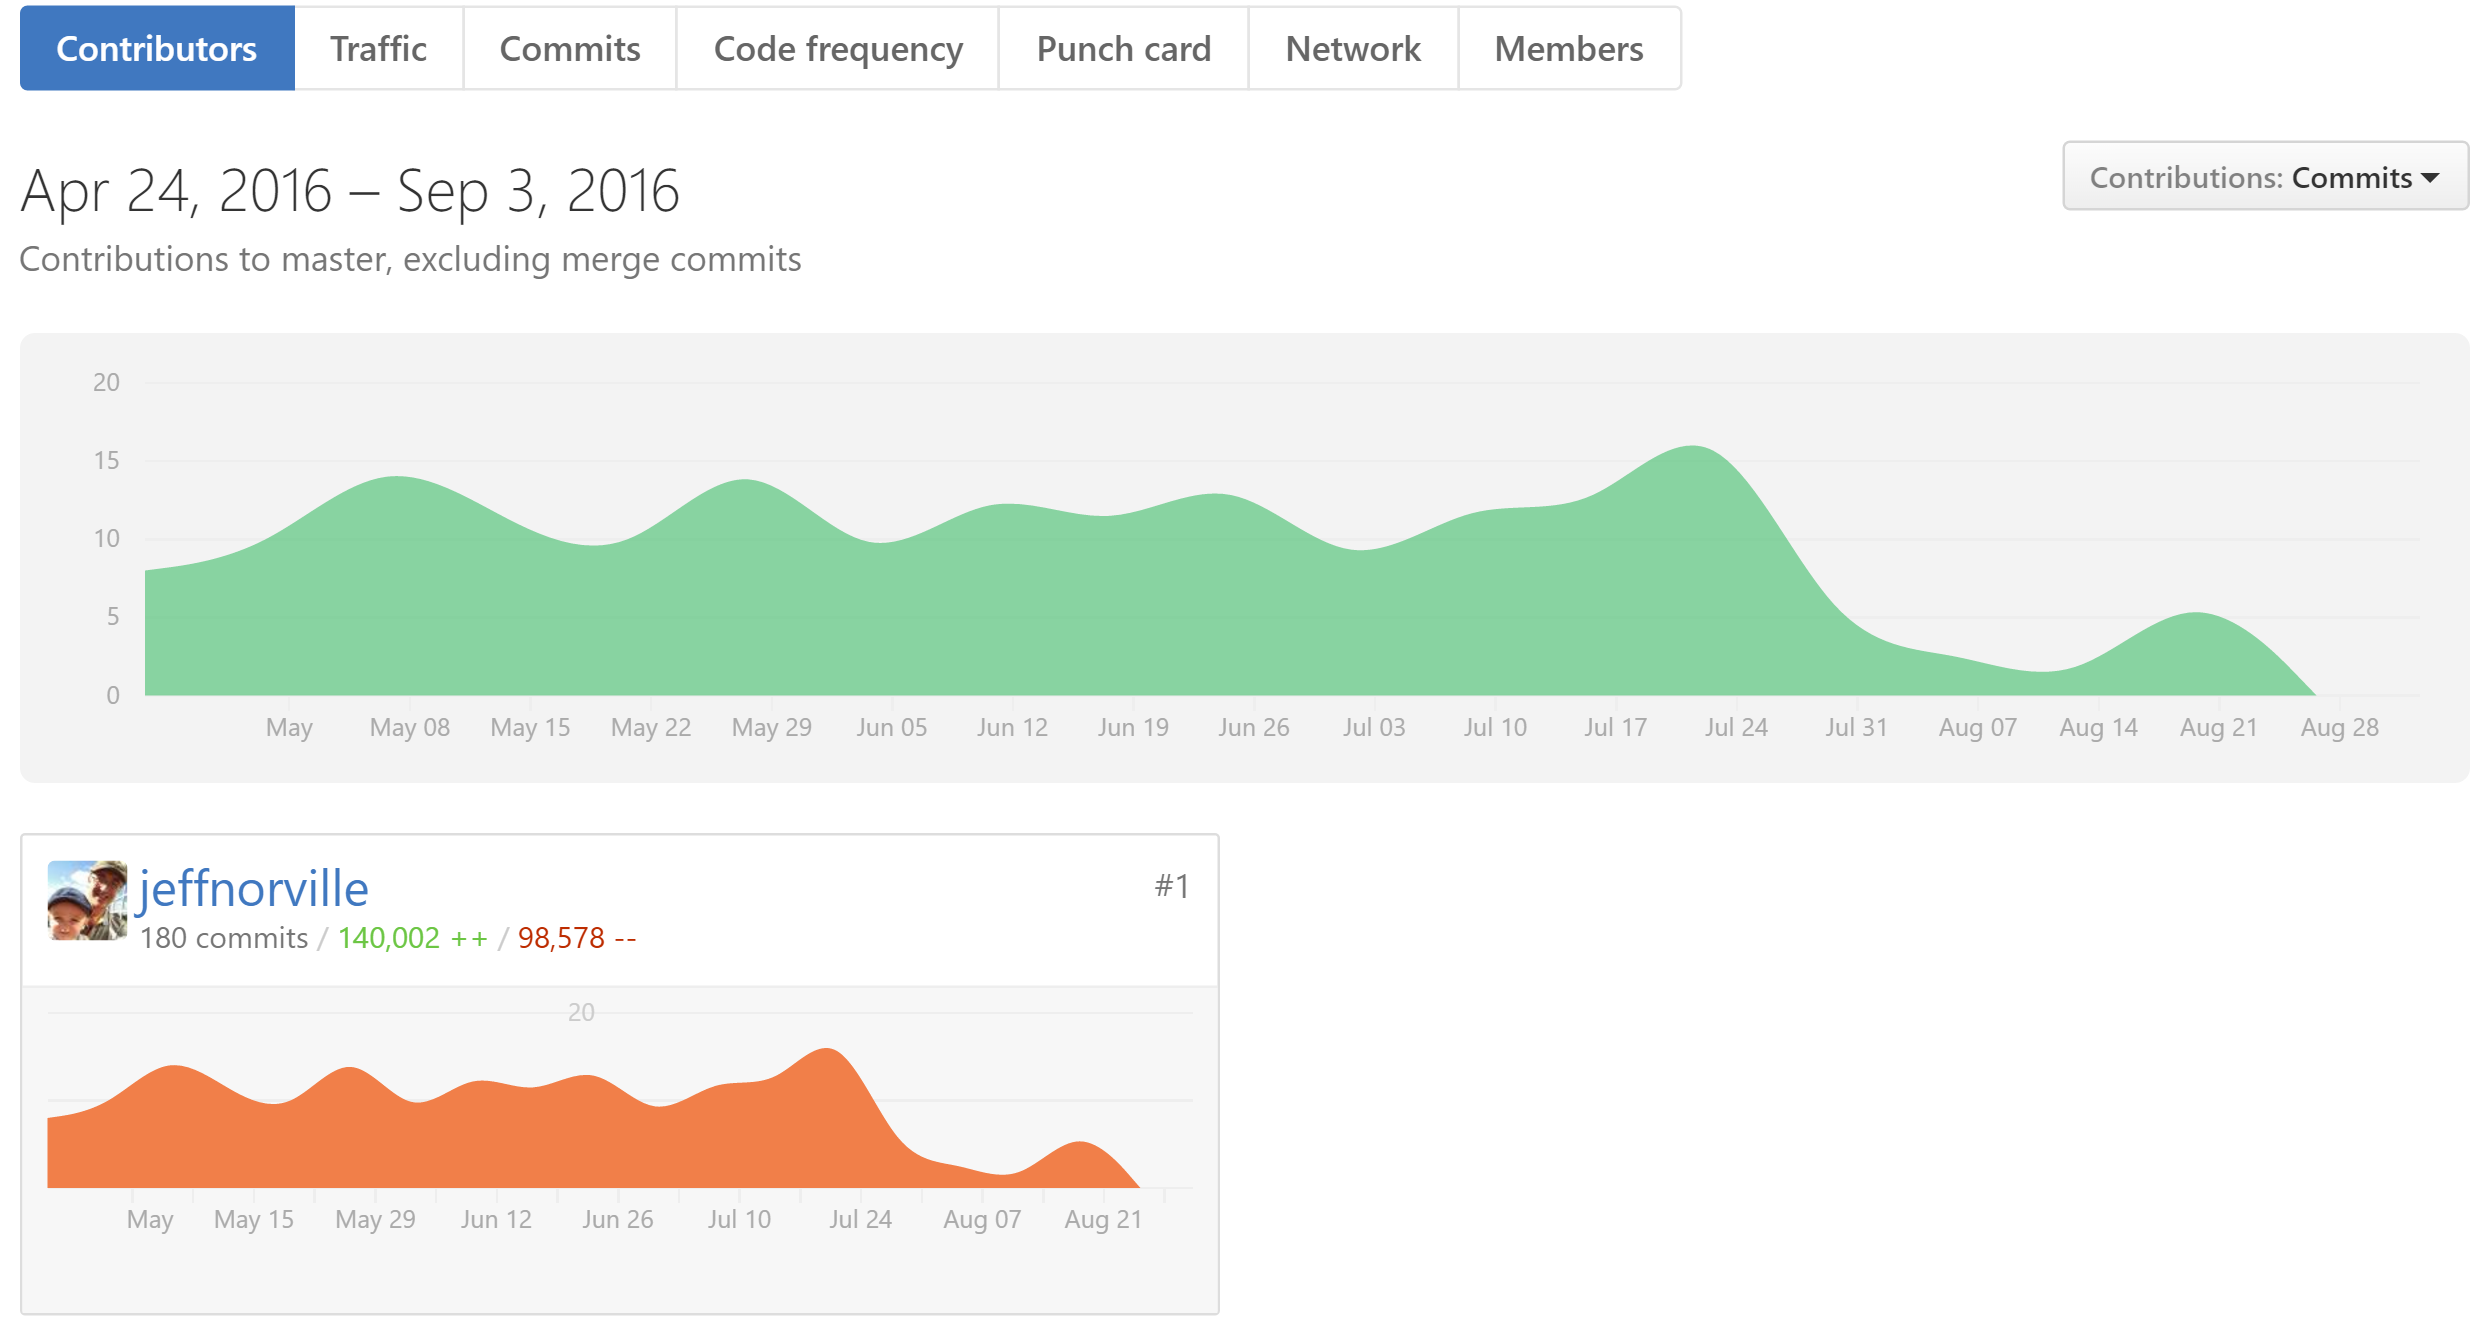
\includegraphics[width=0.8\linewidth]{images/githPlotCommitActivity.png}
%   \includegraphics[width=\linewidth]{boat.jpg} % textwidth
  \caption{my github Activity (shinysb1) during development}
  \label{fig:githubactivity}
\end{figure}

\section{Tools: Shiny by RStudio}

The sections below detail our experience using each tool for this project, so I've followed a repetitive format to include: 1) Options; 2) Compromises; 3) Notations (format specifications for example); 4) Lessons Learned (was this the right tool, or was there a better one?).

The most noticeable tool of the project was RStudio's (a popular IDE, integrated development environment) \textbf{Shiny}, which facilitates interactive webpage design.

\subsection{Options}

There are also options other than R for creating a scoreboard. EVS, for example, is written entirely in Java, a language targeting cross-platform users more than statistics. Options for creating a similar webpage / database framework are also many, from commercial partners like Microsoft's SqlServer database with a c\# middleware and server pages. However, since R began providing Shiny libraries, there are not many systems designed to create a consistent look and feel across data access services to GUI which are based on one language.


\begin{figure}[ht]
\centering
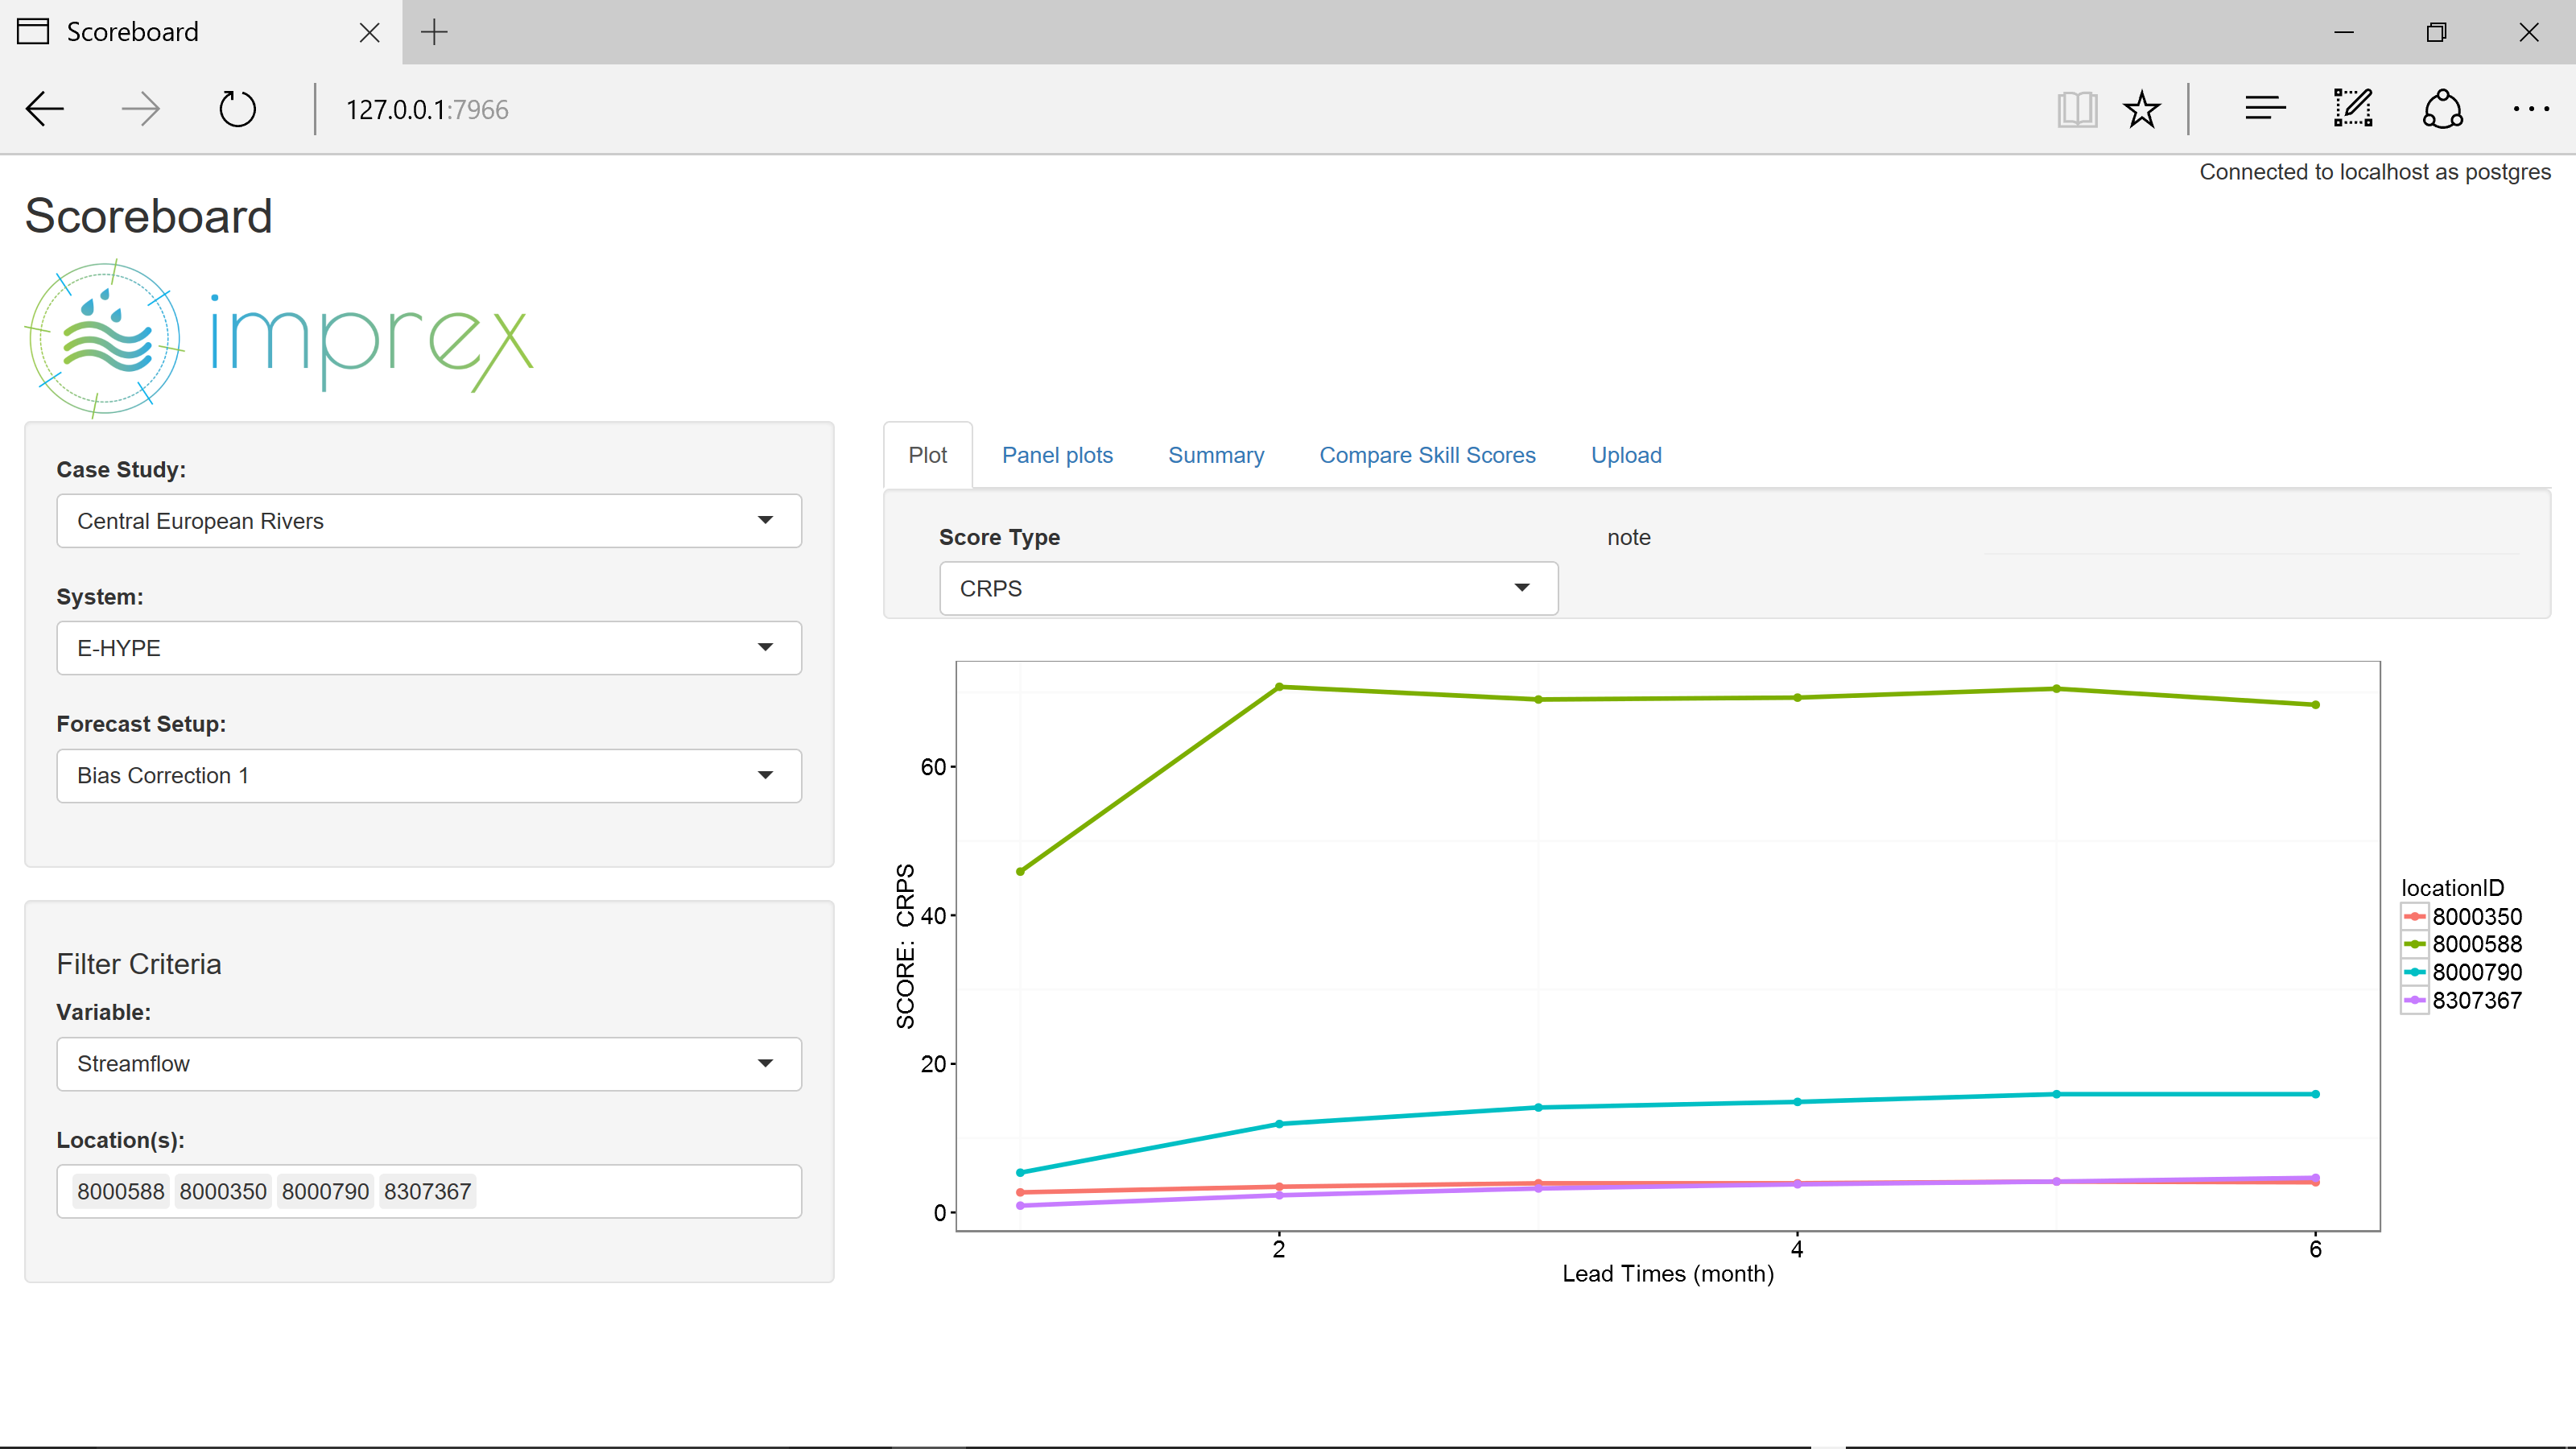
\includegraphics[width=\linewidth]{images/shinPlotCRPS.png}
%   \includegraphics[width=\linewidth]{boat.jpg} % textwidth
  \caption{Scoreboard example}
  \label{fig:scoreboard example}
\end{figure}

\subsection{Compromises}
There are languages which feature richer web-based libraries, and better database integration than R; however for a user-base primarily interested in statistics and numerical solvers, R is not a compromise, but the better solution.

But Shiny as a tool is itself a compromise; it is a high-level language (R) and set of libraries which encapsulate difficult JavaScript, HTML and even database / SQL interfaces beneath a ``familiar'' R interface. The R expert can create dynamic, consistently attractive pages based on existing libraries; and deploy them quickly, without dabbling in the other technologies.

In order to create the pages online one also needs to be connected with a Shiny server; RStudio hosts servers which are free at first (\href{https://www.shinyapps.io/}{www.shinyapps.io}), but there is a cost with increasing usage.

It is also possible to host Shiny servers on any server platform, for example on an inexpensive cloud-based service like Amazon Web Services, or any other variety of enterprise web server.

Once the webpage is is active on a Shiny server, of course, it can no longer read data from the local PostgreSQL database instance on one's computer; it reads only from a database server. PostgreSQL runs on a server too, naturally (AWS also provides a data service). According to the Shiny server documentation reviewed, server performance is best if the database instance and the Shiny server are not running on the same machine (ex with the same processors), as the memory- and processor-intensive operations while generating a large or complicated graphic would compete for the same resources on a shared server.

\subsection{Notations}
Shiny applications are typically split into two executable files: \textit{ui.R} and \textit{server.R}. The overarching goal is to separate the logic of the application from the display -- separating form from content.

Otherwise standard R format applies throughout Shiny.

\begin{minted}{R}
require(dplyr)
require(ggplot2)
toto1 <- filter(toto, locationID %in% basin.list[1:9])
ggplot(toto1, aes(x = leadtimeValue, y = scoreValue)) +
  geom_boxplot() +
  facet_wrap(~ locationID) +
  xlab("Lead Times") + ylab("RMSE Scores")
\end{minted}

\subsection{Lessons Learned}
Uploading data from a web interface to a database is universally a hard thing to do. Shiny does this well, but there's a small risk in loading Rdata files from unknown users: the variable names in the Rdata files aren't controlled, and once they are loaded onto the server space they \textbf{replace variables on the server application of the same name}.

This behavior is documented but not well-respected in the online Shiny community. A solution exists for a "serialized" data connection -- essentially limiting the "Rdata"-like file to one parent entity, and related data objects. This file type is called the RDS filetype, and was our choice in implementing the Data Loader function.

Another problem that remaines to be solved is identifying locations and their proximity. The best alternative to the current selection-box system, which requires a user to select points by a listed name, would of course be to select points from a map. The leaflet R library offers a good interface based on layers (one could overlap different score types as independent layers, selecting groups of points nearby one another, or based on another geographic similarity), but integrating leaflet -- and in particular automating the import of geospatial data by anonymous users -- remains outside the scope of this project.


\section{PostgreSQL}

For our current deployment we used PostgreSQL 9.5, as of publication of this document the latest version is 9.6R1.

A database is simply a collection of data; in the classic computer definition it divides the structure of data (tables, queries, schemas and so on) from the data content itself (records, values). An analog database example might be a file cabinet, with the papers contained within the folder in file drawers the records.

However working a database into the source control workflow, even a high-quality system like PostgreSQL, is more complicated; there is no true source control for a database.

For this reason backups or restores are typically done in two steps:
\begin{enumerate}
\item Backup / Restore Structure
\item Backup / Restore Content
\end{enumerate}

Occasionally people have stored the "data definition language" for the database structure in git. To simplify distribution and maintenance, I split the structure into a file called \textit{"structureDATE.backup"} and \textit{"contentDATE.backup"}, where the DATE is replaced by the creation date. For now these are stored on my github account, but as they are the largest binary file I will find another system to distribute them.

PostgreSQL is installed with its own GUI called pgAdmin (Figure \ref{fig:pgAdmin}). This utility can create backups and restores directly; the user (with database permissions, ex password) can view the structure directly, and write short data requests to view contents using Structured Query Language (SQL).

\begin{figure}[H]
\centering
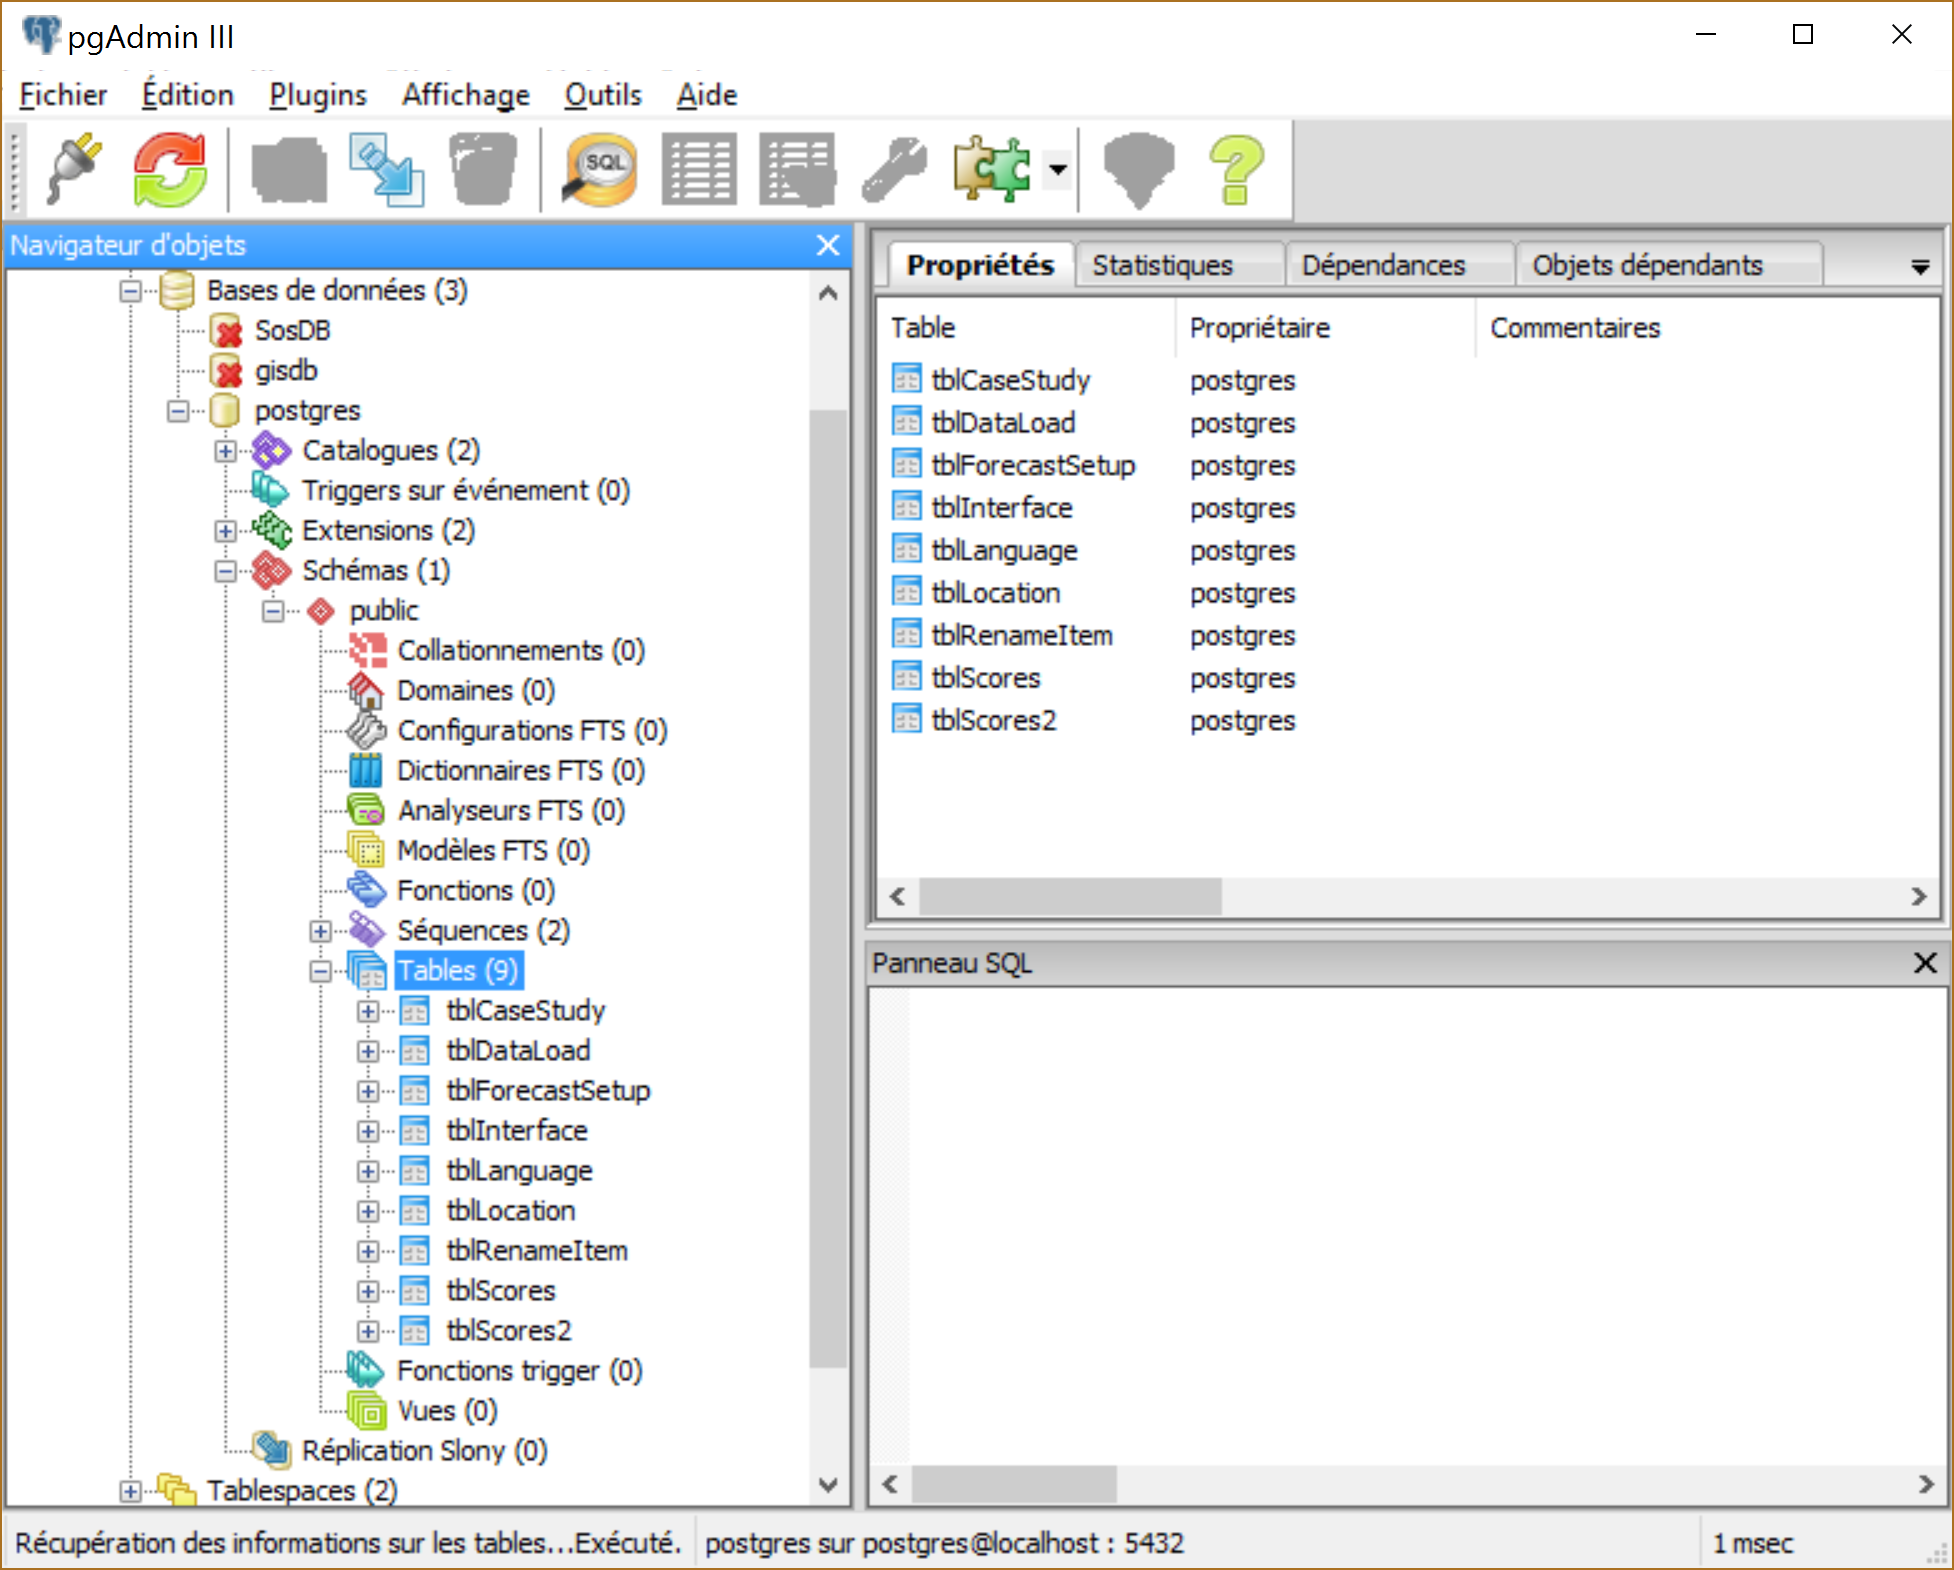
\includegraphics[width=0.7\linewidth]{images/pgAdmin1.png}
  \caption{PostgreSQL pgAdmin GUI interface}
  \label{fig:pgAdmin}
\end{figure}

\subsection{Options}

Many alternative databases and file systems exist as an alternative to PostgreSQL:

\begin{enumerate}
\item Sun Microsystems MySQL
\item Oracle database
\item Microsoft SqlServer
\item NetCDF data files
\item SOS database (used by ECMWF and implemented recently)
\end{enumerate}

One of the reasons ECMWF and other GIS or data-driver model entities rely heavily on PostgreSQL is it accommodates an open source utility called PostGIS, which integrates spatial data in the database. Similar functionality can be had in Oracle and Microsoft systems, but as exorbitant costs (for an academic institution).

As noted under the list of alternative options to this database, the \href{http://52north.org/473-52-north-sos-4-3-7-now-available}{SOS Database} is actually a framework which runs on a combination of PostgreSQL, PostGIS, and several other open-source components (Tomcat, Apache tools). ECMWF recently implemented this to make available their water level forecasts; as of this time their version does not make available observations at all (personal communication Paul Smith, 23 august 2016).

% * <jeff@jnorville.com> 2016-09-09T11:50:25.532Z:
%
% Notes on comparing NetCDF and a multidimensional array database for large hydrologic datasets...
% thesis by Haicheng Liu, TU Delft, 29 octobre 2014
%
% ^.

While we hope there are many users of the system, we have anticipated accommodating limited types of data: numeric, date, and integer values, which will be received and processed as score files. We request spatial data (location information as coordinates) but that is optional; currently we do not have a method to upload shapefiles to the database (a potential request from team members).

During imports where our default data schema cannot be matched, or the partner does not use R in-house, we can build a custom import tool. With each successive data import the import method becomes "smarter", adding a mapping for our database and allowing future automated imports. This does not exist today.
% * <jeff@jnorville.com> 2016-09-09T11:52:07.339Z:
%
% Since many collaborators already use R, we have developed a small file specification that, if matched, may be uploaded directly to the scoreboard database.
%
% ^.

\subsection{Compromises}

Our system needs to account not for time-series data in every case, but also for data on different timescales; for this reason we've included two different "scales" of dates in the database, technically a "no-no" for a database administrator, but a necessary evil to accommodate our potential users.

Currently the database accepts ``point based'' geographic coordinates in one coordinate reference system, but many users work with shapefiles (polygons). There are add-on modules available for PostgreSQL which work with shapefiles, but we did not implement them for this project.

\subsection{Notations}

A short example of a database creation script:
\begin{minted}{SQL}
CREATE TABLE "tblScores"
(
  "row.names" text,
  "locationID" text,
  "scoreValue" double precision,
  "forecastType" text,
  "dateValue" date,
  "datePartValue" numeric, -- valid numeric values: 12 (month), 51 (week)
  "datePartUnit" text, -- valid values: "month", "week"
  "leadtimeValue" integer,
  "leadtimeUnit" text, -- daily weekly monthly
  "scoreNA" boolean, -- if scoreValue == NA then TRUE
  "scoreType" text, -- lookup to other table of forecast types
  "modelVariable" text,
  "dataPackageGUID" text
)
\end{minted}

\subsection{Lessons Learned}

I made a number of errors with PostgreSQL implementation, most of which were due to being out of date with the tools or general complexity.
% * <jeff@jnorville.com> 2016-09-09T11:55:40.144Z:
%
% Discuss: RDBMS can be all in, all out, OR hybrid
%
% ^.

\begin{enumerate}
\item SQL's date type column is the fastest and most-efficient index to use when querying large datasets by actual dates; however, I initially overlooked that the vast majority of our data is NOT timeseries data
\item Amazon Web Service for remote hosting - due to the installation being slightly more complicated than I anticipated, the free AWS tier was quickly exceeded
\item PostgreSQL "series" datatype (automatic sequence) not compatible with R's write table function
\end{enumerate}

As noted, although our first dataset relied heavily on daily values, and due to it's size benefitted from using the ``date'' datatype in the database, the majrity of our score datafiles do not have daily date values; additionally, using a date field for a month value when that value represents perhaps 30 years of months is incorrect, and misleading to future code maintainers.

We solved this by implementing both a date field and a datePart field, which is paired with datePartUnit. One or the other is mandatory for each record, but they are also exclusive of one another. This means a record will either have a date: ``2011-08-04'' ; or an entry in datePart (``34'') paired with datePartUnit (``week'').

For the last point, PostgreSQL ``series'' datatype remains a sticky issue. We rely on automatically-generated indexes when loading new datafiles into the PostgreSQL tables, which is a standard operation, and I modified the RPostgreSQL library to work with the datatype on local installations. However, updates to the RPostgreSQL library -- or installations to new servers, other laptops -- do not respect the local modification. To date the maintainer of that part of the source code library has not accepted the proposed change (easiest path). 


\section{R and RStudio}

\subsection{Options}
For graphical output and statistical models, R seems to be winning the open-source -- and even among the proprietary -- tool sets in popular circulation today.

Base R and R IDEs are often confused, the IDEs are a developer convenience -- the R base installation may be accessed directly from the command line.

Popular IDEs other than RStudio include \href{https://sourceforge.net/projects/tinn-r/}{Tinn-R}, \href{https://cran.r-project.org/web/packages/Rcmdr/index.html}{RCommander}, \href{http://www.eclipse.org/downloads/packages/release/Luna/R}{Eclipse}, and \href{https://beta.visualstudio.com/vs/rtvs/}{Microsoft's Visual Studio}.

\subsection{Compromises}

RStudio is available for Linux and Mac as well as Windows, and it is a stable product. However, it is fair to say using a language designed for statisticians to create a web interface is a strange concept to many outside the R universe!

\section{Conclusion on Technology Decisions}
% \subsection{Lessons Learned}
The general workflow and technology using R and Shiny make a lot of sense for this workflow. There are many examples of such simple interfaces, hosted both by RStudio and through their forums. The vast majority of the Shiny pages I reviewed, however, use either a static datafile on the server or ``scrape'' data dynamically from another service or page (weather, elections, etc). There are not as many database-driven Shiny websites today.

While the database interfaces to Shiny seem somewhat under-developed (lack of support for auto-incrementing series, error handling is limited, lack of awareness of database ``state''), the database part of this project is too important to disconnect the two.

Another option could be to write a custom set of libraries to speed up communication from the R Shiny scoreboard and the database directly. Because of the nature of R, the authors have opened up their source code to facilitate that approach to programmers who need it.

%########################################################################
% Design part
%########################################################################

\part{Scoreboard Design}

\begin{figure}[ht]
\centering
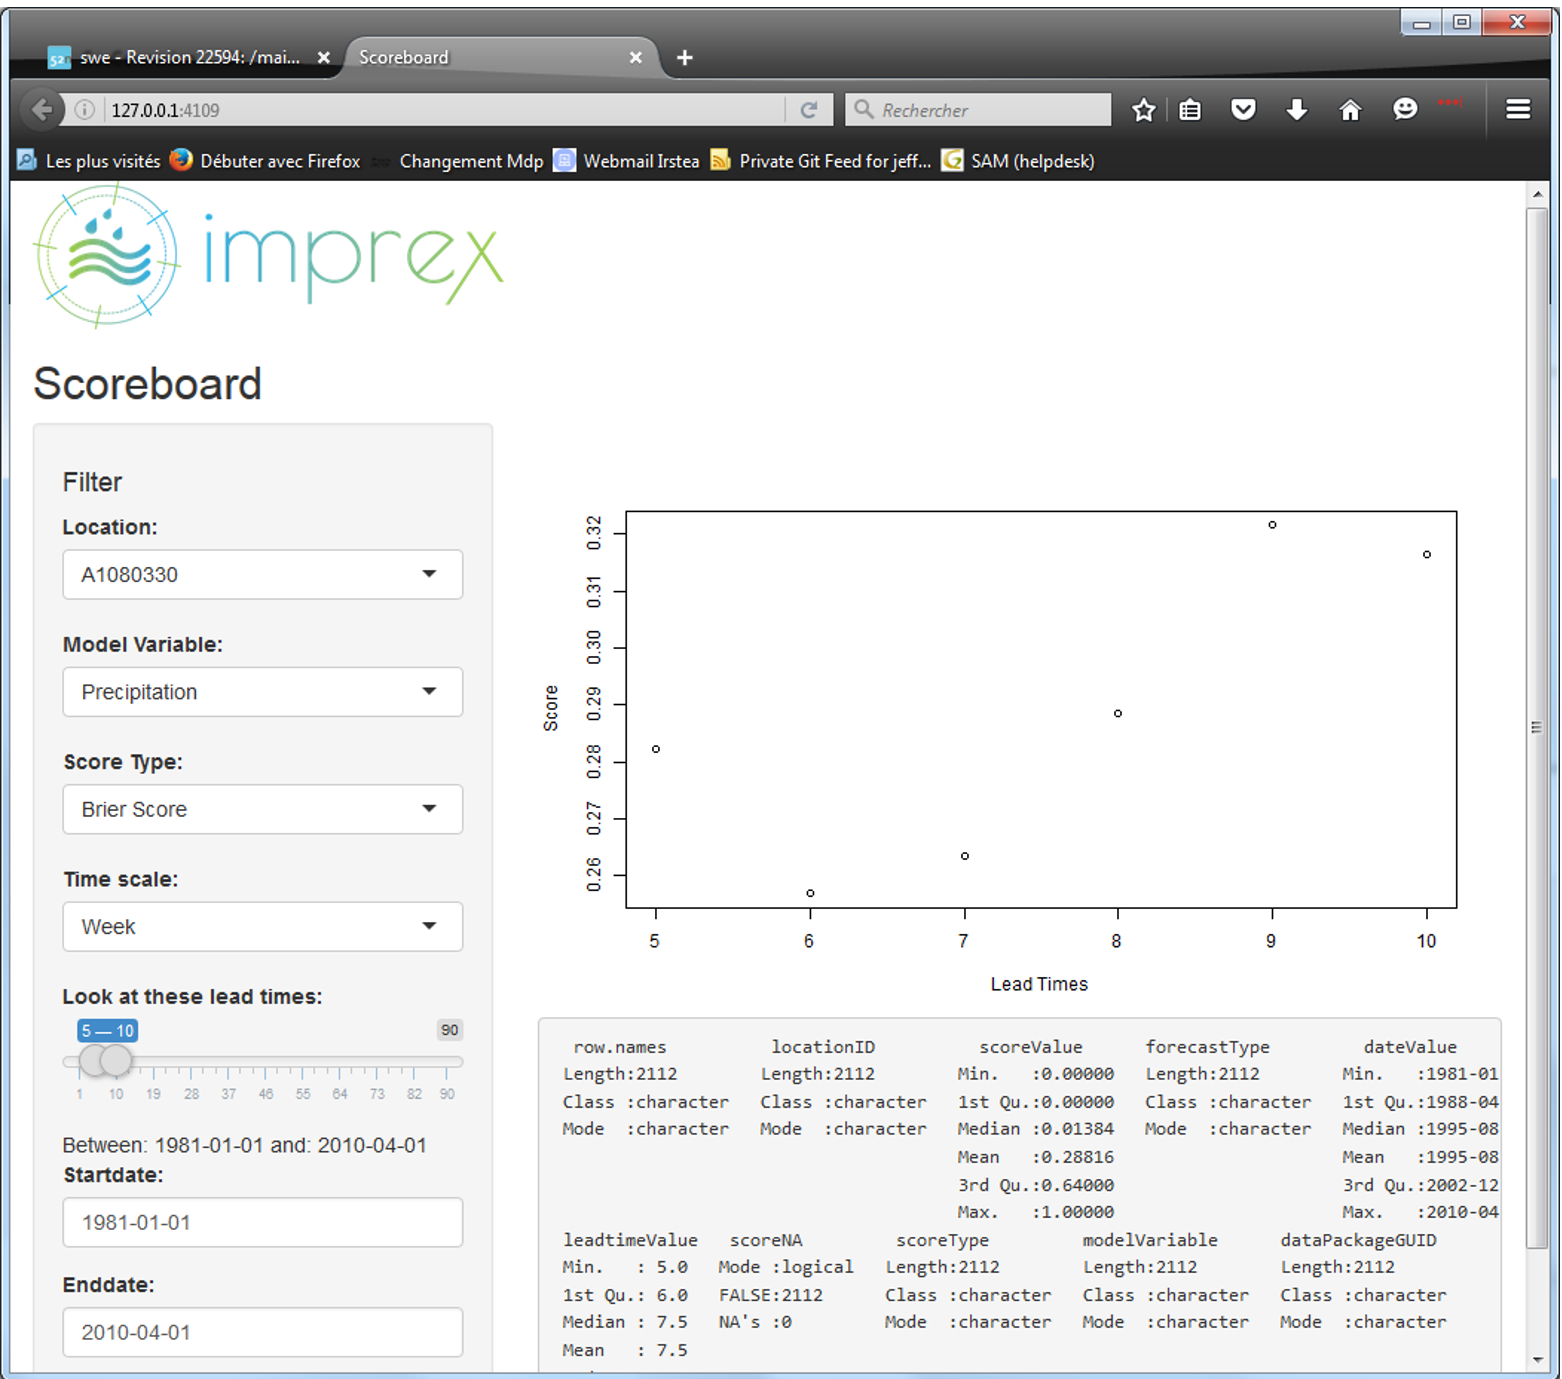
\includegraphics[width=0.8\linewidth]{images/sbdV1v21notes.png}
%   \includegraphics[width=\linewidth]{boat.jpg} % textwidth
  \caption{Scoreboard v1}
  \label{fig:scoreboard v1}
\end{figure}

As noted elsewhere, a "universal" scoreboard was an undefined concept. Here are three iterations using our chosen toolchain (RShiny, postgresql) to build test frameworks.

\section{Version 1 - Working With Daily Values}
%v21 notes
My first "scoreboard" was based on the first data we received -- a big data set with daily values over 30 years, lead times to 3 months (90 days), for 16 French catchments. That dataset included four model data types: two different bias corrections for streamflow and precipitation.

\begin{figure}[!ht]
\centering
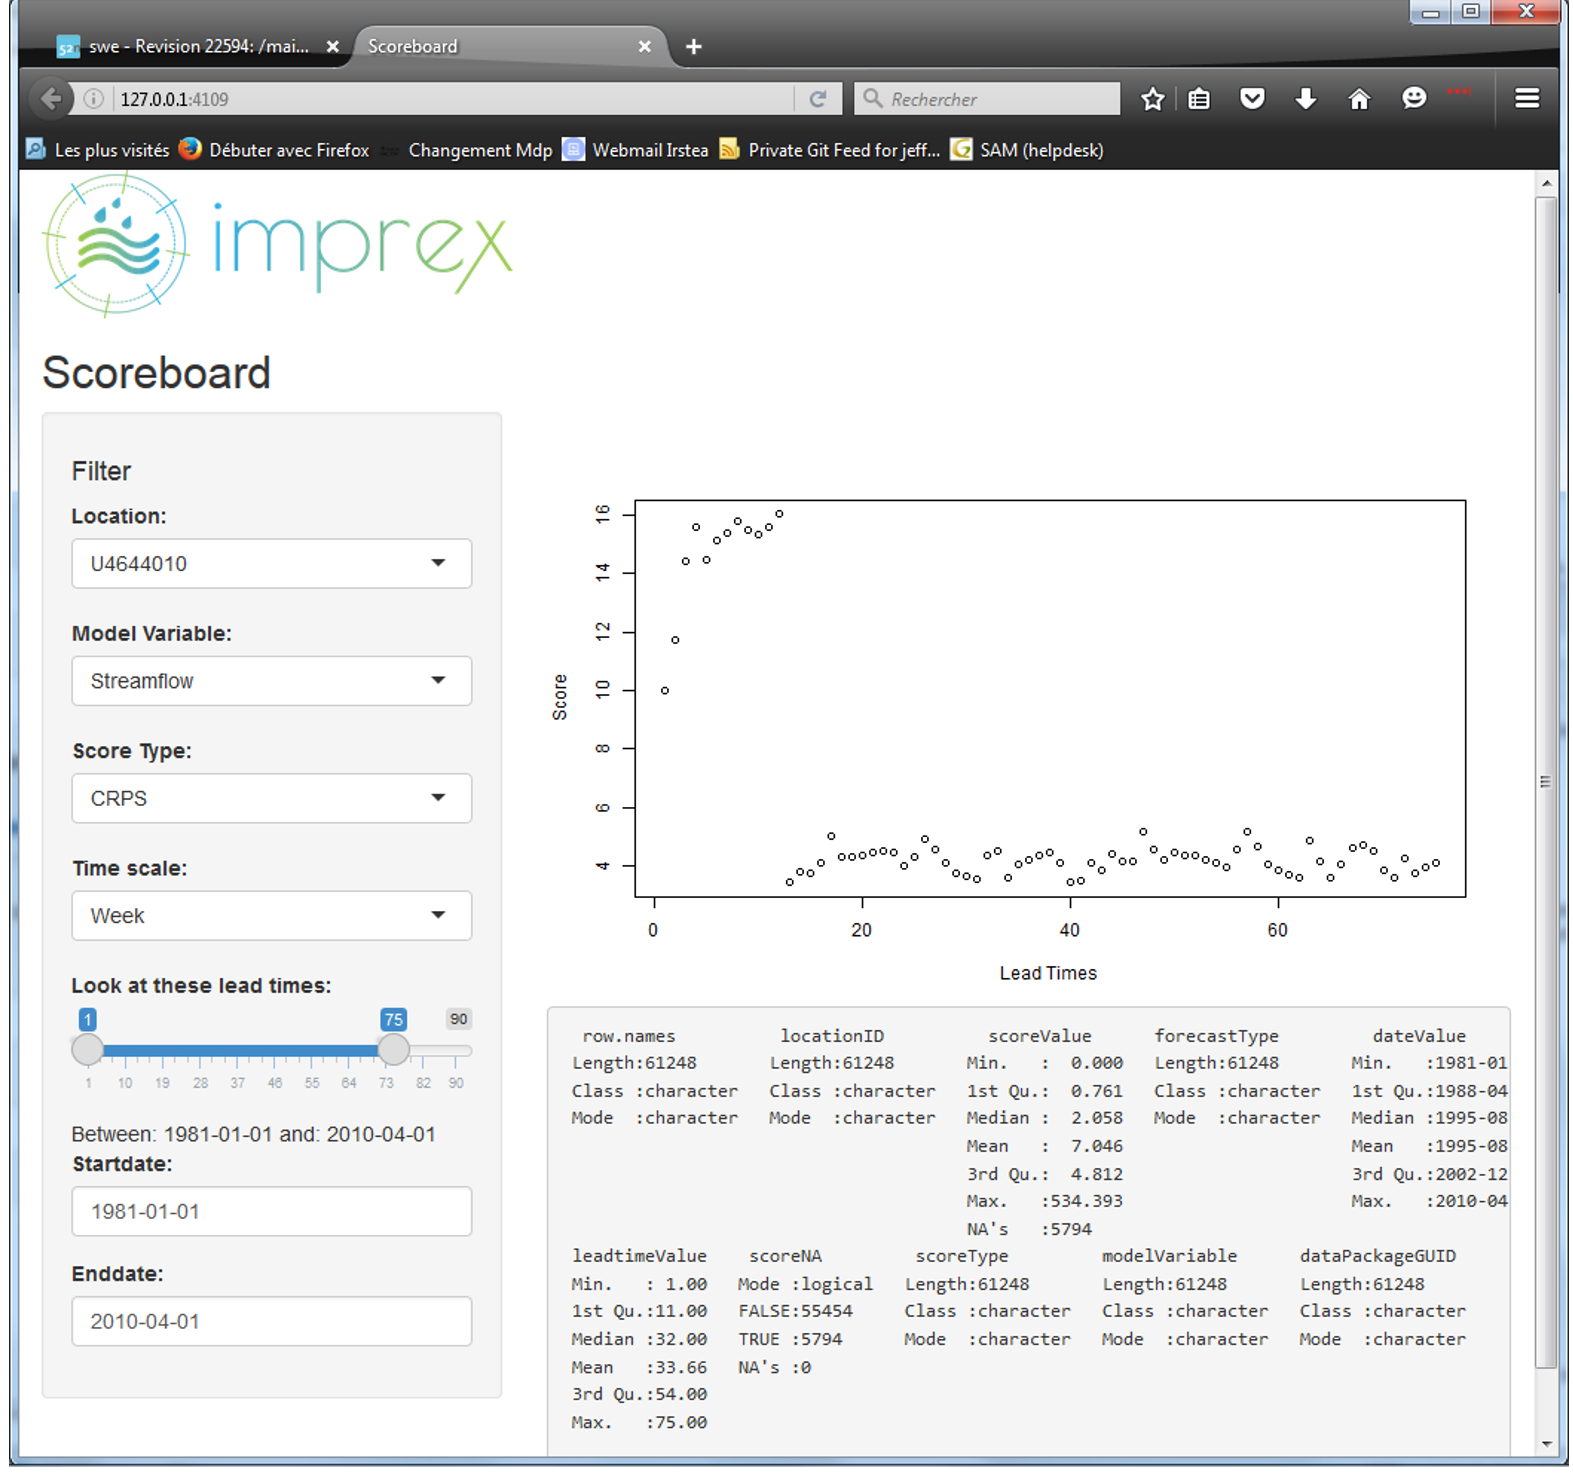
\includegraphics[width=0.8\linewidth]{images/sbdV1v21notes2.png}
%   \includegraphics[width=\linewidth]{boat.jpg} % textwidth
  \caption{Scoreboard v1, note leadtimes 1:75 selected by "slider"}
  \label{fig:scoreboard v1.2}
\end{figure}

Figure \ref{fig:scoreboard v1} shows the navigation bar, left, where the user may change Location; Model Variable; Score Type; Time Scale; then there's a slider to select between one and 90 lead times, and a date range selector in case one wants to tune comparisons of different data sets. 

This plot shows one score type over just six lead times, and the standard R "summary" function below the plot was useful to check selections during development.

Figure \ref{fig:scoreboard v1.2} shows the first scoreboard again but with more lead times selected (1:75). This first version did not accommodate multiple selects (even on Location), but that was due to a "bug" in the Shiny library I was using: I could use 2:n values to search, or one value, but the change between the two was quite awkward. I solved this problem in future scoreboards.

\section{Version 2 - Displaying Details}

The second version incorporated the same controls (since we were using the same first dataset) with nicer graphics, namely the  \gls{ggplot2} library and default color scheme. One big enhancement based on ggplot: we added confidence intervals on every data point. Another was including a function to return confidence intervals and standard error when running monthly averages on the entire dataset.

The error bars were included because every plotted point in Version 1, above, is a mean monthly value taken on 30 years of daily values compared against lead time. In order to "display" the depth of the data, including an R function to count the values, collect basic stats, and return a dataframe which made the error bars easy to add and modify made sense. In this image the bars are 95\% confidence intervals.

\begin{figure}[H]
\centering
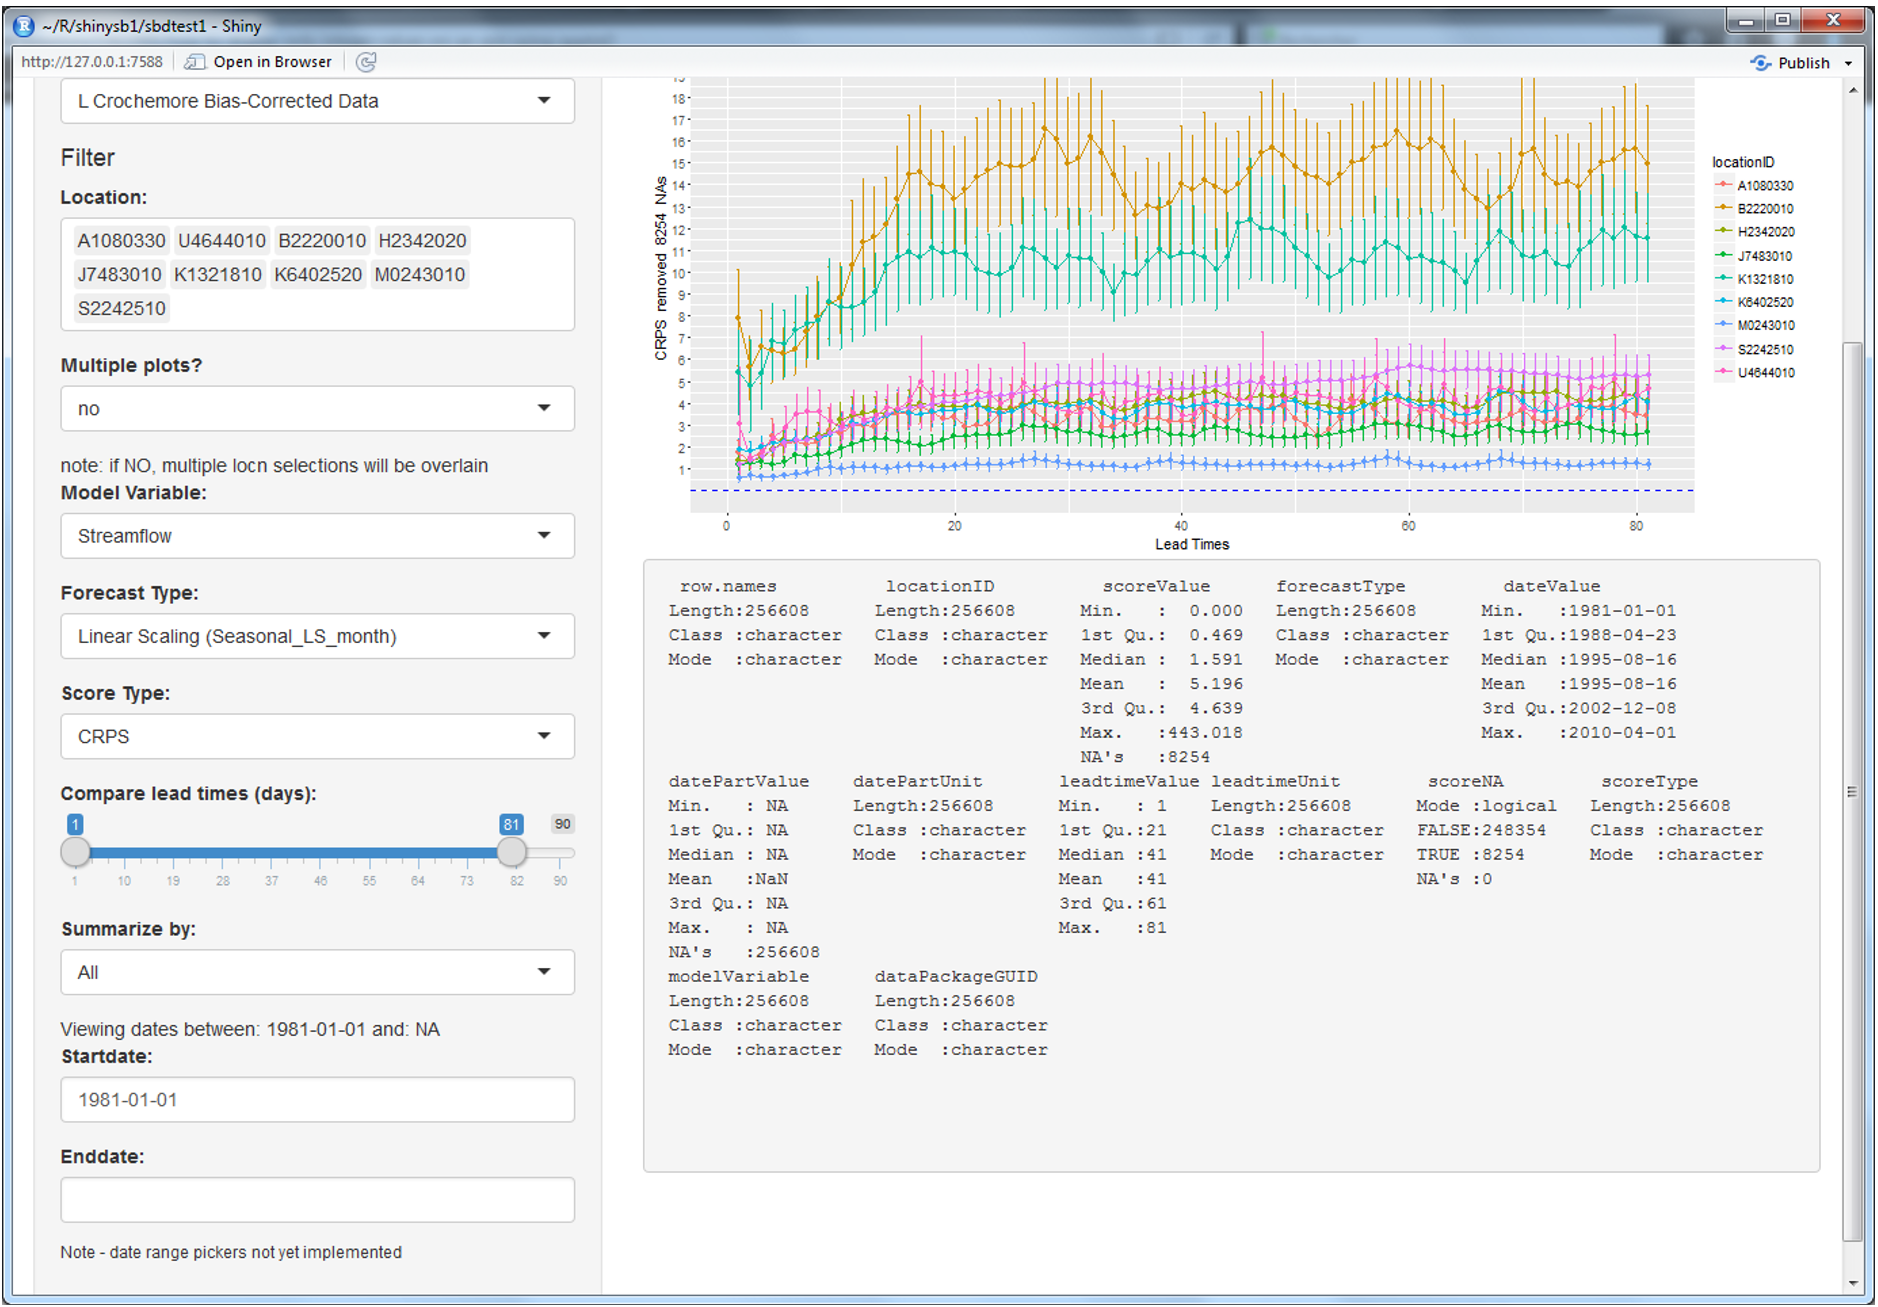
\includegraphics[width=0.7\linewidth]{images/sbdV2v24notes.png}
%   \includegraphics[width=\linewidth]{boat.jpg} % textwidth
  \caption{Scoreboard v2, note color change in plot}
  \label{fig:scoreboard v2}
\end{figure}

However, the error bars were, in fact, less interesting than other comparisons we could perform between locations, between score types.

\section{Version 3 - Data Mining}

The third (and latest) scoreboard version looks quite different than the first two, partly because we received two new data sets that were quite different from the first.

While the initial dataset had \textbf{daily} values including daily projections of lead time, the next two datasets were somewhat more processed. Values were already averaged by month, then sliced across years, creating one value which represented nearly a thousand values in the first dataset. (This varies slightly, as not each dataset started and finished on the same date.)

To illustrate the differences in volumes of data, see Table \ref{tbl:origDatasetCompare} below.

When using daily datasets (\textit{dataset 1}), more data are stored. Receiving score data averaged to one month from the entire 30 year range (\textit{dataset 2}) means we have fewer data to process before makng the display. In fact, we received double the 3 month lead time noted in(\textit{dataset 2}), for 6 months of lead time (see \textit{dataset 2 extended}), which allows for deeper comparisons.

Combining the two resolutions of data in the display required some changes to the way the database schema handled date values, but in this version the resolution of data is nearly transparent to the user (the more compact datasets response a bit more quickly).

\begin{table}[h]
\centering
\begin{tabular}{@{}lccccr@{}}
\toprule
 & Interval & Years & Values per Year & Lead Times & Total \\ \midrule
dataset 1 & daily & 30 & 365 & 90 & 985500 \\
dataset 2 & month avg & 30 & 12 & 3 & 1080 \\
dataset 2 extended & month avg & 30 & 12 & 6 & 2160 \\ \bottomrule
\end{tabular}
\caption{Size Comparison by Dataset Resolution}
\label{tbl:origDatasetCompare}
\end{table}

While we set out to define our own data standards, we want to encourage team members to send us their score data without too much rework. We changed assumptions that team members would send us daily values, as 1) it does not add much to the scoreboard product, and 2) it will "fill up" the database very rapidly to import daily values.

As of the writing of this document I have not yet aggregated the original dataset to monthly values to match the other two.

Table \ref{tbl:selectOptions2} is our outline for creation of the three main "plot" panels of the Verification Scoreboard: 
\begin{itemize}
\item Plot (see Figure \ref{fig:isb1})
\item Panel Plot (see Figure \ref{fig:isb2})
\item Compare Skill Scores Plot  (see Figure \ref{fig:isb4})
\end{itemize}

The \gls{scoreboard-user} may choose a Forecast System, a Setup, a single Model Variable, but any number of Locations.

More complex is the decision matrix under Compare Skill Scores tab: the user is creating their own skill score based on the chosen score as a "reference"; they are limited to choosing either two Systems and one Setup, or one System allowing two Setups. This programming is taken care of in Shiny.

% If you use beamer only pass "xcolor=table" option, i.e. \documentclass[xcolor=table]{beamer}
\begin{table}[h]
\centering
\begin{tabular}{@{}lccccc@{}}
\toprule
 & \multicolumn{1}{l}{System} & \multicolumn{1}{l}{Forecast Setup (System)} & \multicolumn{1}{l}{Locations} & \multicolumn{1}{l}{Variable} & \multicolumn{1}{l}{Score} \\ \midrule
Plot & \cellcolor[HTML]{FFFFFF}1 & \cellcolor[HTML]{FFFFFF}1 & \cellcolor[HTML]{FFFFFF}n & \cellcolor[HTML]{FFFFFF}1 & \cellcolor[HTML]{FFFFFF}1 \\
Panel Plots & \cellcolor[HTML]{FFFFFF}1 & \cellcolor[HTML]{FFFFFF}1 & \cellcolor[HTML]{FFFFFF}n & \cellcolor[HTML]{FFFFFF}1 & \cellcolor[HTML]{FFFFFF}n \\
 & \cellcolor[HTML]{FFFFFF}1 & \cellcolor[HTML]{CBCEFB}2 & \cellcolor[HTML]{FFFFFF}n & \cellcolor[HTML]{FFFFFF} & \cellcolor[HTML]{FFFFFF} \\
\multirow{-2}{*}{Skill Comparison Plots} & \cellcolor[HTML]{CBCEFB}2 & \cellcolor[HTML]{FFFFFF}1 & \cellcolor[HTML]{CBCEFB}all & \multirow{-2}{*}{\cellcolor[HTML]{FFFFFF}1} & \multirow{-2}{*}{\cellcolor[HTML]{FFFFFF}n} \\ \cmidrule(lr){2-4}
\end{tabular}
\caption{Choices for User Selections in latest Scoreboard}
\label{tbl:selectOptions2}
\end{table}

Additionally, if there are more than twelve Locations selected, the line plot changes to a series of box-whisker plots. See below, Scoreboard Testing, for an introduction to the Skill Comparison Plots.

%########################################################################
% Sixth part
%########################################################################
\part{Scoreboard Testing}

\section{Score Data Used for Testing}

We received three data deliverables from two different weather centers, ultimately loading one from each center to the IMPREX database for testing purposes: SMHI and ECMWF.

\subsection{SMHI Score Data}

Swedish Meteorological and Hydrological Institute of Sweden (\href{http://www.smhi.se/en}{SMHI}) sent us score data calculated from their E-HYPE model. E-HYPE is a Pan-European hydrological model for seasonal streamflow forecasts that runs over 35000 sub-basins (median resolution=215 km\textsuperscript{2}) across all of Europe.

\begin{figure}[H]
\centering
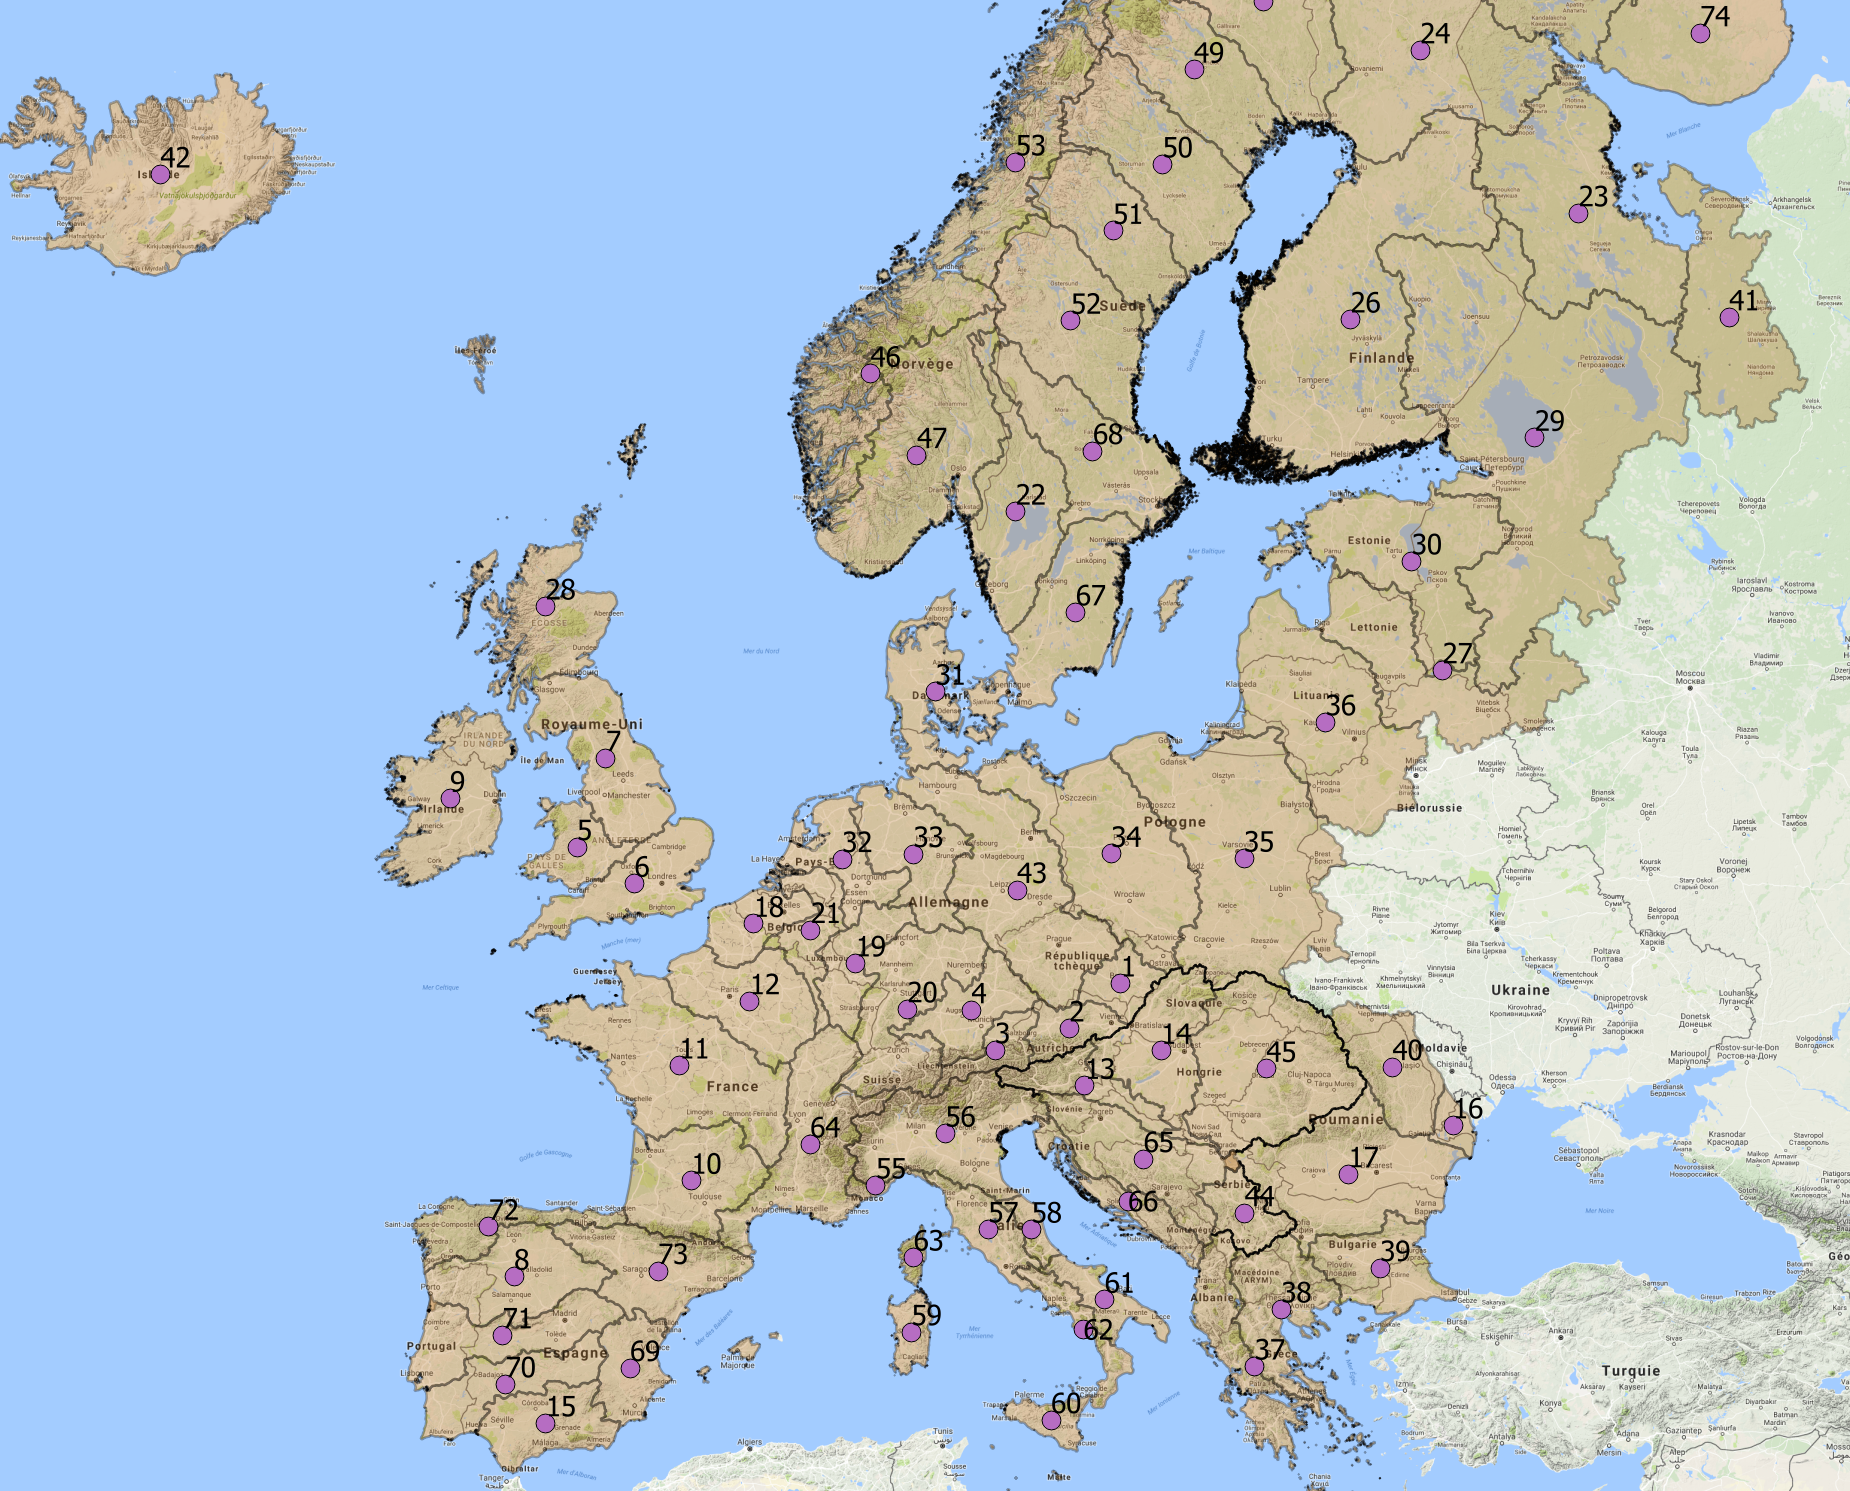
\includegraphics[width=0.8\linewidth]{images/gisEHYPEcentroids.png}
%   \includegraphics[width=\linewidth]{boat.jpg} % textwidth
  \caption{E-HYPE Shapefile Centroid Data}
  \label{fig:EHYPEdata}
\end{figure}

Daily streamflow forecasts were obtained using the System 4 seasonal precipitation forecasts from ECMWF as input to the E-HYPE hydrological model. The streamflow forecasts were verified by SMHI with a variety of numerical scores, including Brier score, correlation, CRPS, RMSE, and related skill scores.

The E-HYPE score data were provided in RData file format. It contained scores and skill scores for 825 stations in Europe. The file was about 50 MB and contained scores for each month of the year, 6 lead months and each station (i.e., 12*6*825 data points per score).

\subsection{ECMWF Score Data}

\gls{Sys4-EFAS} data was provided by the European Centre for Medium-Range Weather Forecasts (\href{http://www.ecmwf.int}{ECMWF}). Score data come from the evaluation of seasonal streamflow forecasts issued by EFAS (\href{https://www.efas.eu/about-efas.html}{European Flood Awareness System}).

\begin{figure}[H]
\centering
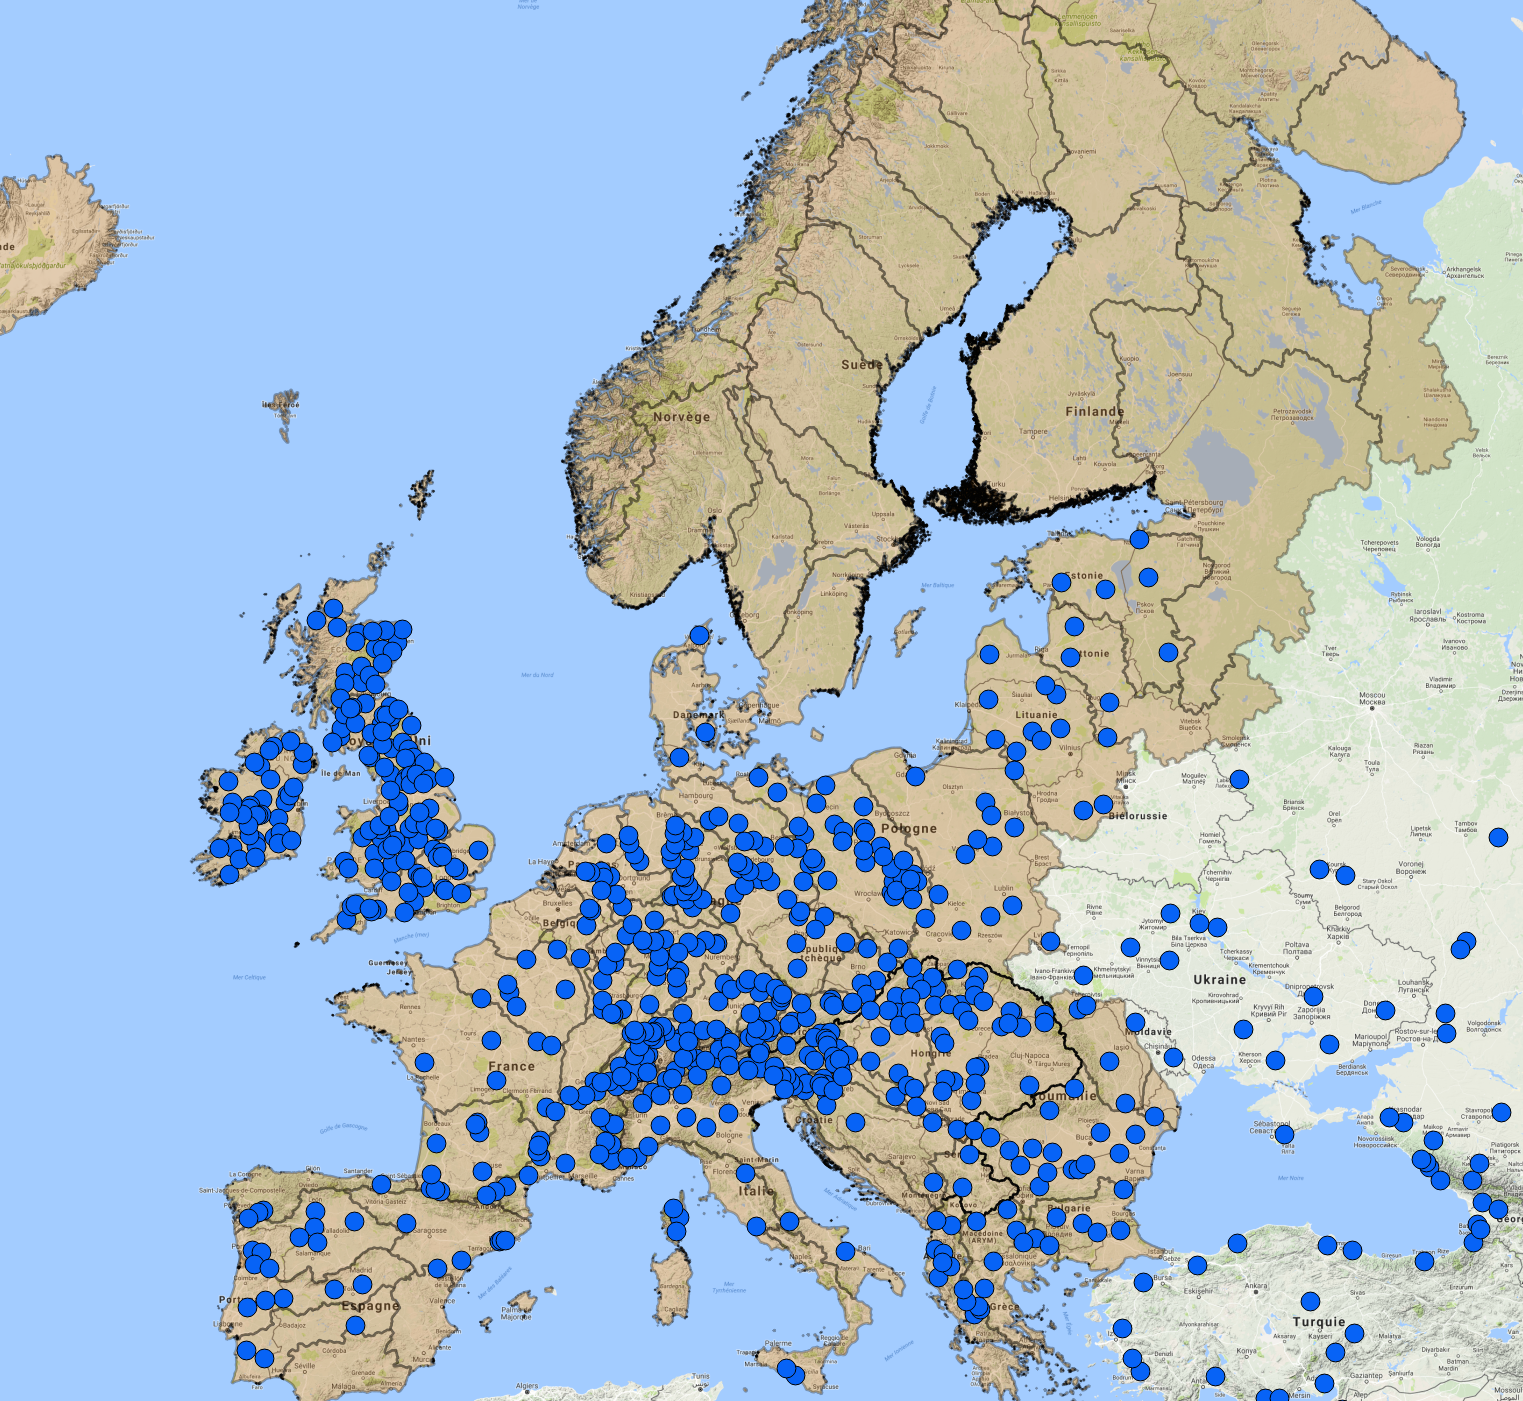
\includegraphics[width=0.8\linewidth]{images/gisEFASpoints.png}
  \caption{ECMWF Point Data}
  \label{fig:ECMWFdata}
\end{figure}

Daily streamflow forecasts were obtained using the System 4 seasonal precipitation forecasts from ECMWF as input to the daily LISFLOOD hydrological model, following its set up in Europe for the EFAS project. LISFLOOD is a GIS-based, distributed hydrological rainfall-runoff-routing model. It is run for all of Europe on a 5x5 km grid. Streamflow is simulated on a pixel basis.

The streamflow forecasts were verified by ECMWF and we have collected CRPS values for the score database. The score data were provided in text file format for 74 basins over Europe. The scores are average scores over all the years of data, for each month for which the forecast is made and each month of lead time (up to 7 months). We have received score values for each basin (not for a station as in the E-HYPE data).  As it was explained to us, these scores come from the quality evaluation of average monthly discharge values over each basin. Daily discharges were first spatially averaged over each pixel inside the basin area, and then temporally averaged over a month, before proceeding to the forecast verification. Shape files were also provided for the geographical location of the basins.

Note that the EFAS LISFLOOD model uses a custom global projection; in order to reproject EFAS points into WGS84, the standard system for our scoreboard, a conversion was necessary.

Additionally, in order to compare locations between these two datasets, I used a QGIS to find nearest neighbor points, and renamed the EFAS points to share the same name as their nearest-neighbor EFAS locations. This issue would be better resolved in R, which has a number of geospatial libraries available to either allow actual spatial queries in Shiny, or to create some pilot points which share similar-enough geographical information as to be useful comparing forecast systems.

%\begin{verbatim}
%+proj=laea +lat_0=48 +lon_0=9 +x_0=0 +y_0=0 +a=6378388 +b=6378388 +units=m +no_defs
%\end{verbatim}

% * <jeff@jnorville.com> 2016-09-09T13:13:45.542Z:
%
% \subsection{Other Score Datasources}
% ECMWF also recently published an online observation consumption tool which publishes their model data as "predictions" using a SOAP or REST service through the SOS database products (North52 description TODO). 
%
% ^.

\subsection{Testing Results: Screen Captures}

In this section we walk through several use-cases of the Verification Scoreboard.

The navigation features are consistent throughout the application, with minor exceptions. The user begins by selecting a Case Study, all nine of which are defined by the IMPREX project. Central European Rivers is our default choice and where most of our test data is located.

The user is then presented with all possible Systems, or Forecast Systems; in the test database we can chose from E-HYPE and EFAS SYS4. Depending on that selection, the next field ``Forecast Setup'' is populated with valid selection choices. Finally, the selection box ``Model Variable'' is populated from prior selections, and the user can typically chose between precipitation, Temperature, and Streamflow. During testing only Streamflow data have been loaded.

Now the interface can create a simple plot once the user selects one or more locations. The user may also change the current Score Type above the plot; in this version all Score Types are shown each time, rather than a selection of valid values from the database.

\begin{figure}[H]
\centering
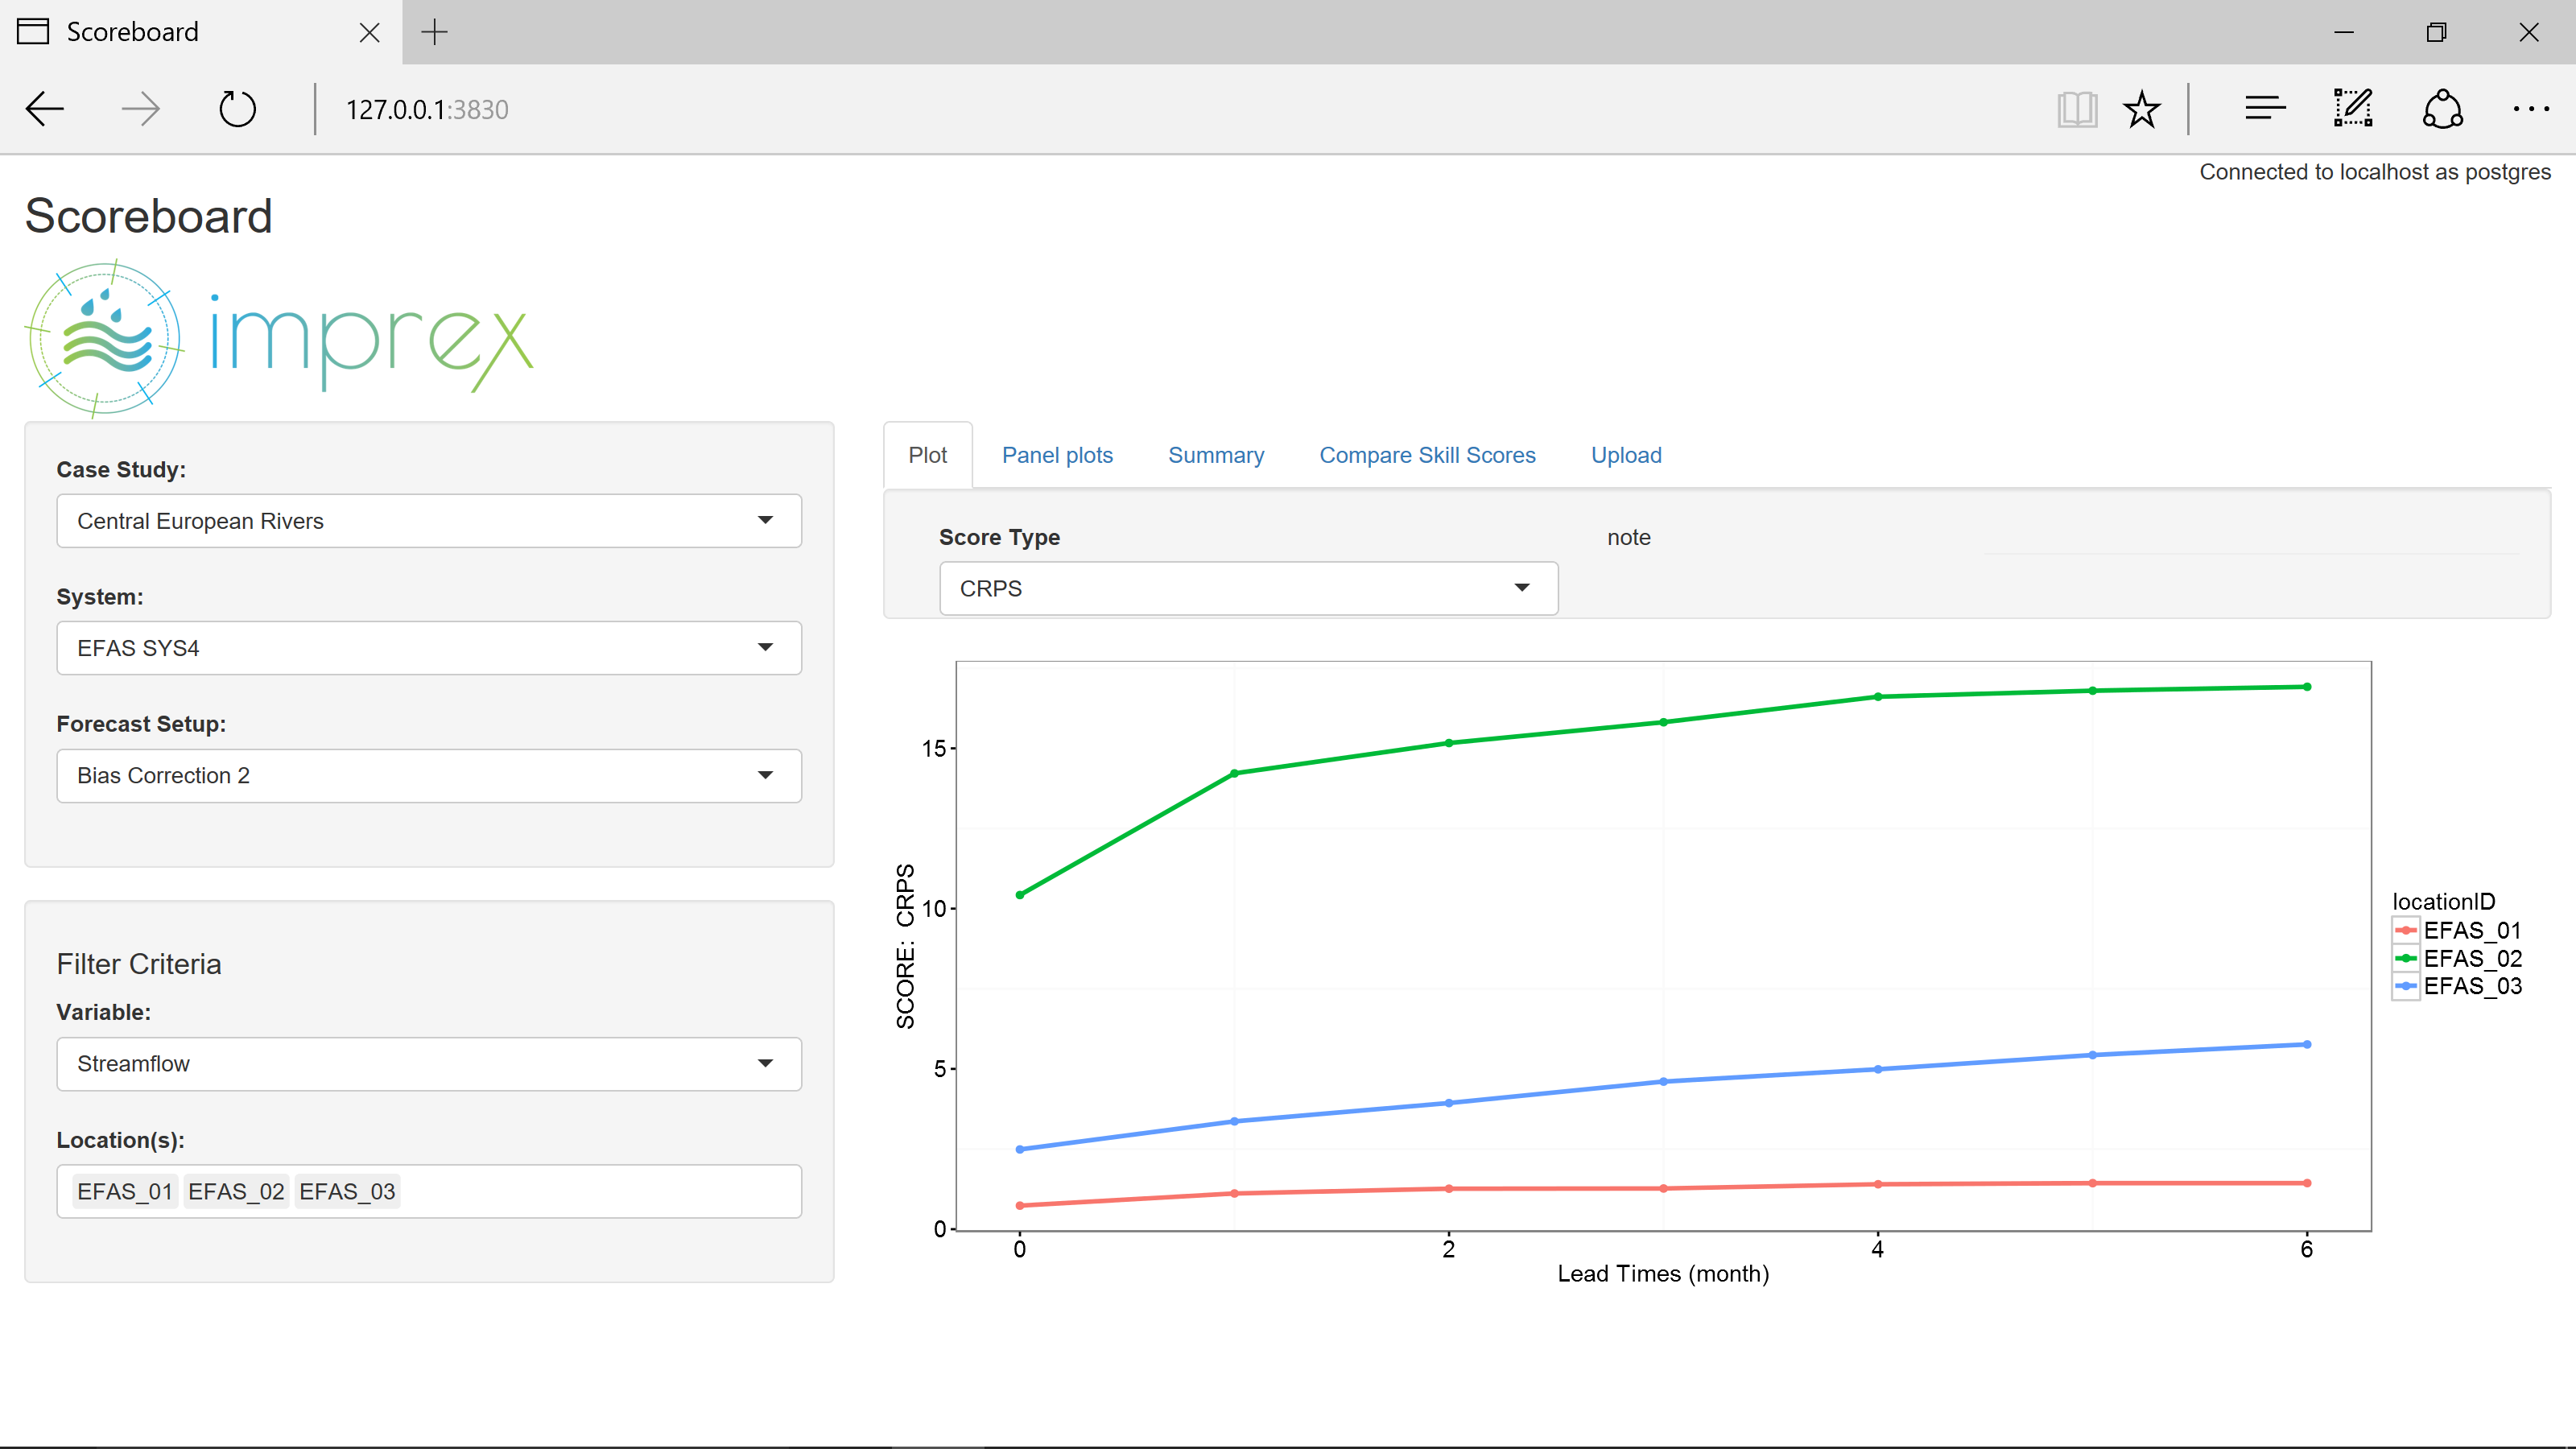
\includegraphics[width=0.85\linewidth]{images/isb1.png}
  \caption{Scoreboard Plot function}
  \label{fig:isb1}
\end{figure}

A small legend appears to the right of the plot to indicate which selected location matches each curve. As with all figures in this scoreboard, the X axis is always the lead time of the forecast scores. As shown in this screenshot, and logically, the CRPS scores increase over lead times; note that a higher CRPS score indicates an increase in the (square of the) difference between observed and predicted values, so a lower value is better. Typically a forecast of today or the next month will be better than one for five or six months from now.

The user may switch directly to the Panel Plot next, which will display the same locations but change the default scores to be: CRPS Skill Score; Brier Skill Score; and RMSE Skill Score. This default behavior is because the only way to hold all variables equal to directly compare scores is to compare skill scores. Other scores are weighted on flow volume, or the size of the basin, or other factor related to a specific location.

Since the database did not have skill scores for these values, I added CRPS in order to plot figures. In stead of the plots being overlain the user sees sequential plots.

In the event there are multiple locations AND multiple scores, the matrix of plots grows in the X and Y direction, respectively.

\begin{figure}[hb]
\centering
<<<<<<< HEAD
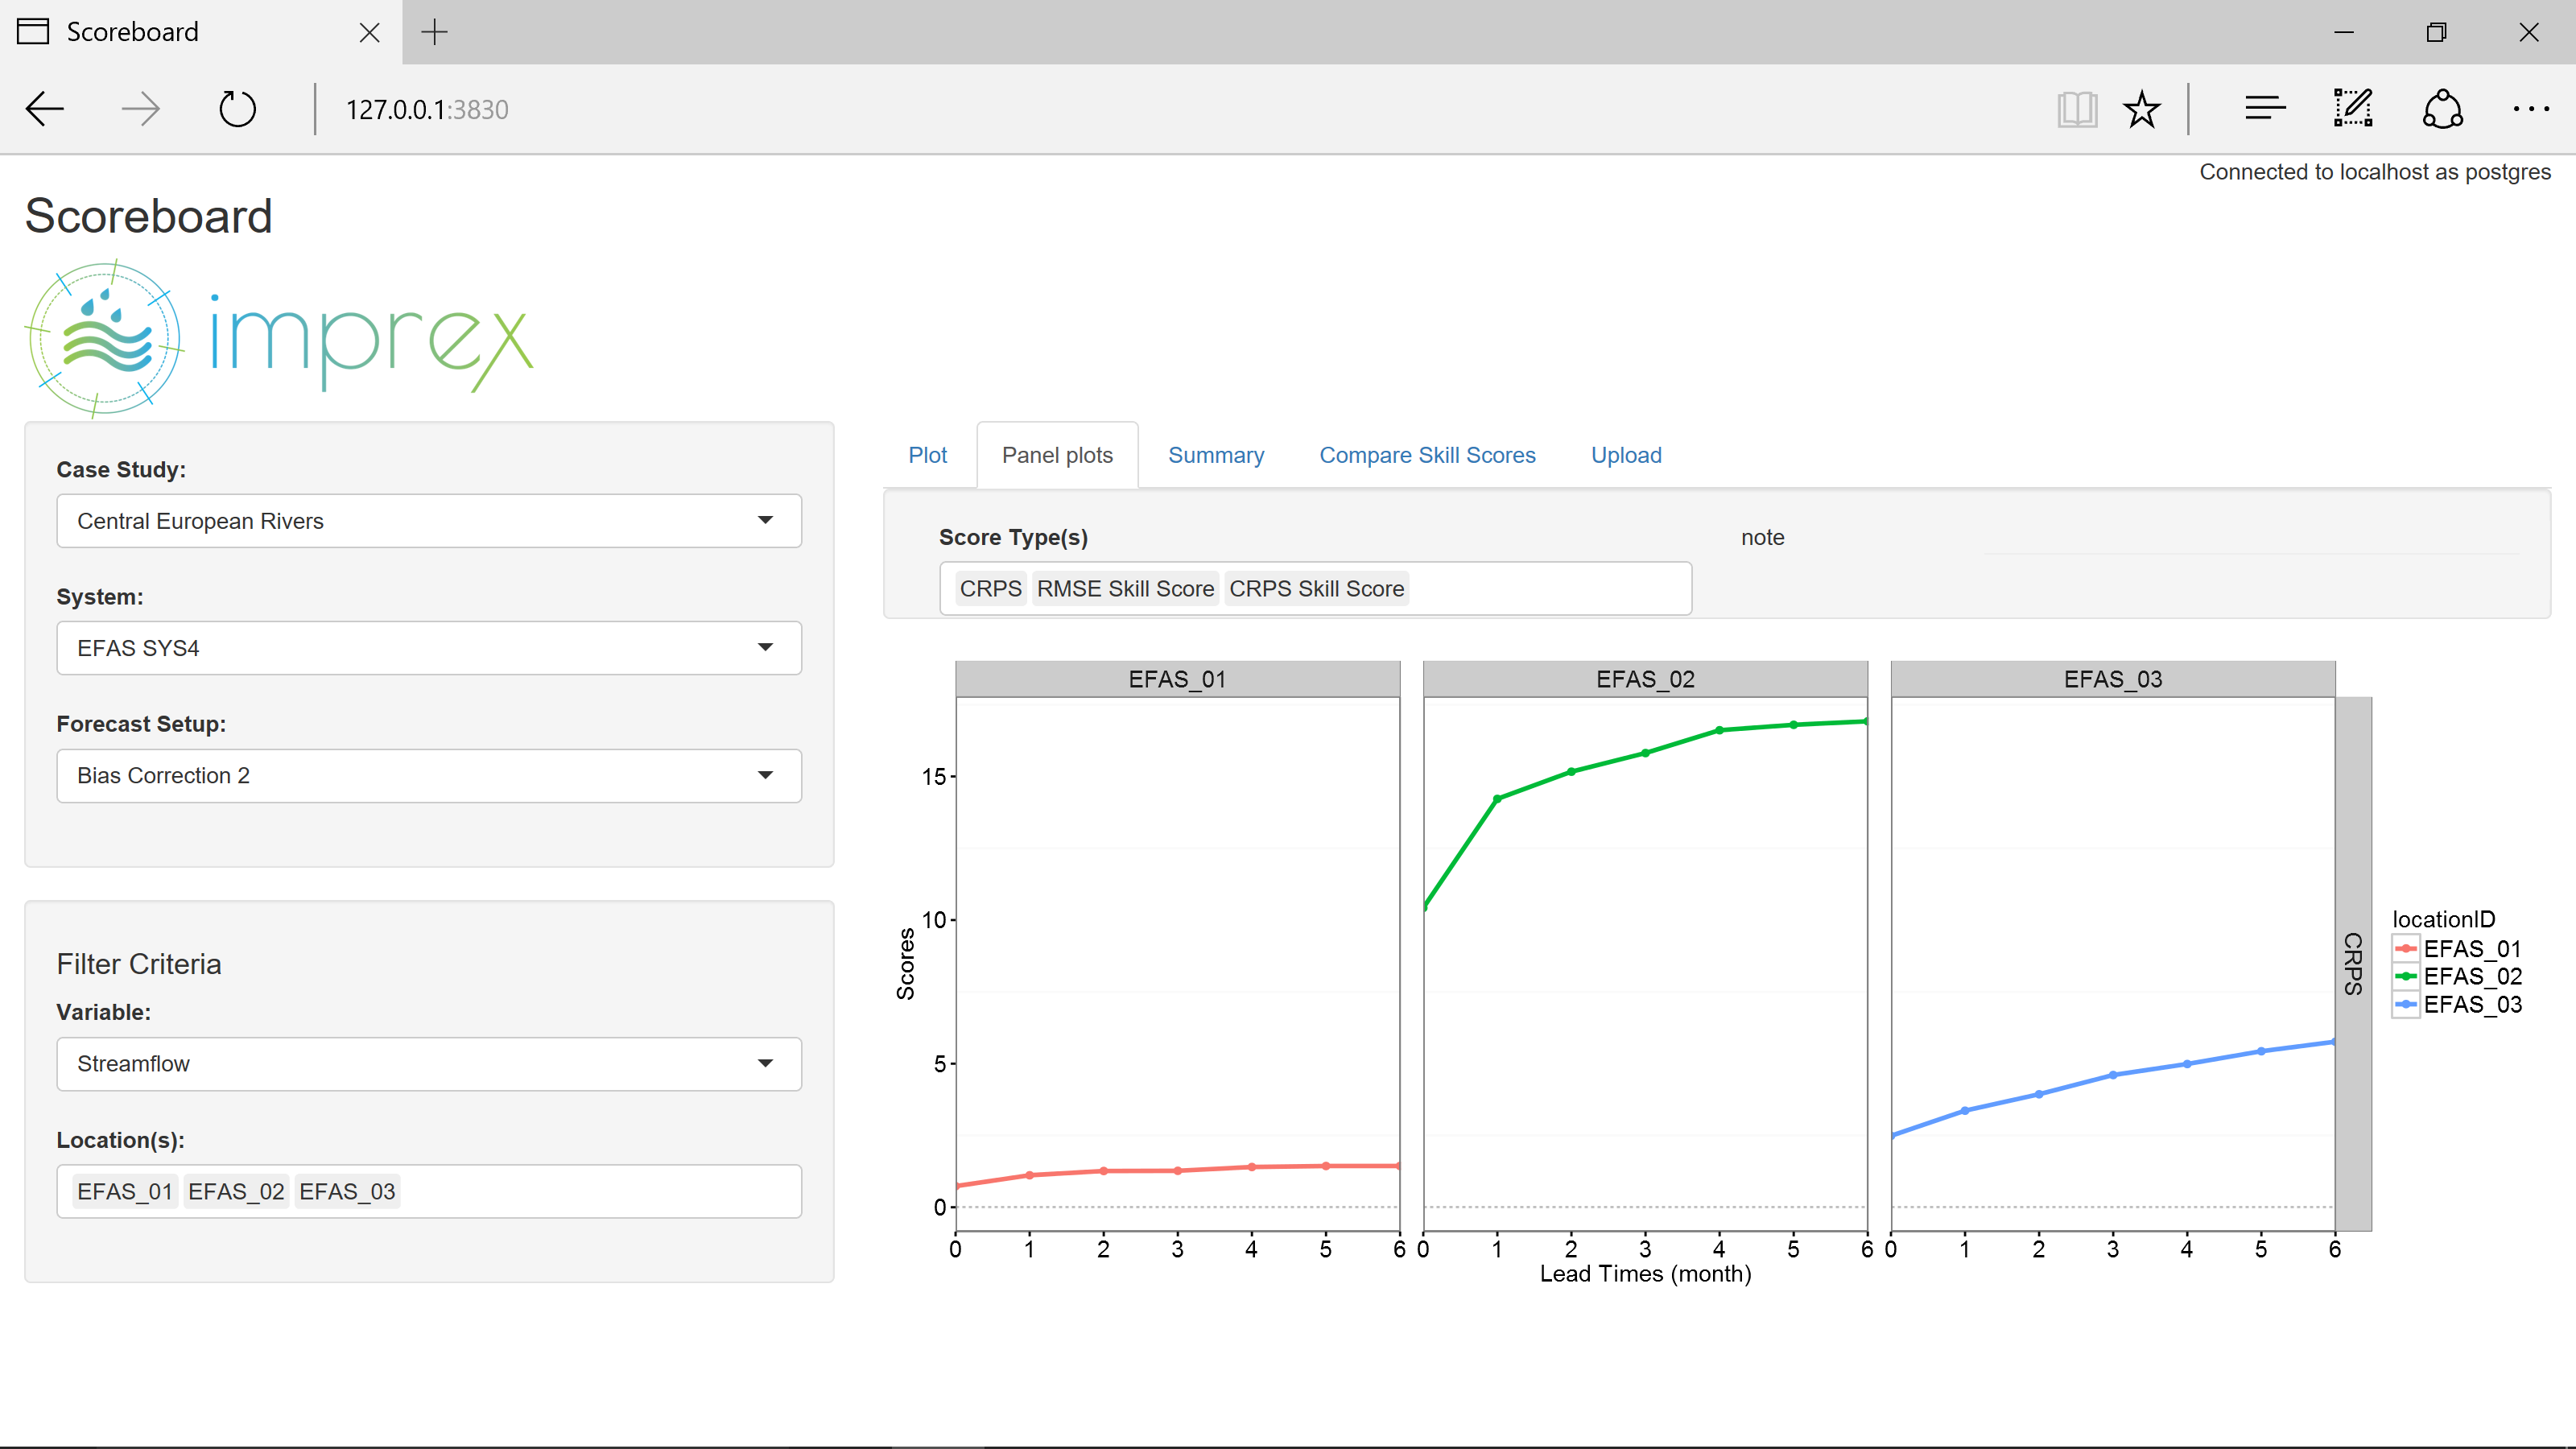
\includegraphics[width=0.80\linewidth]{images/isb2.png}
=======
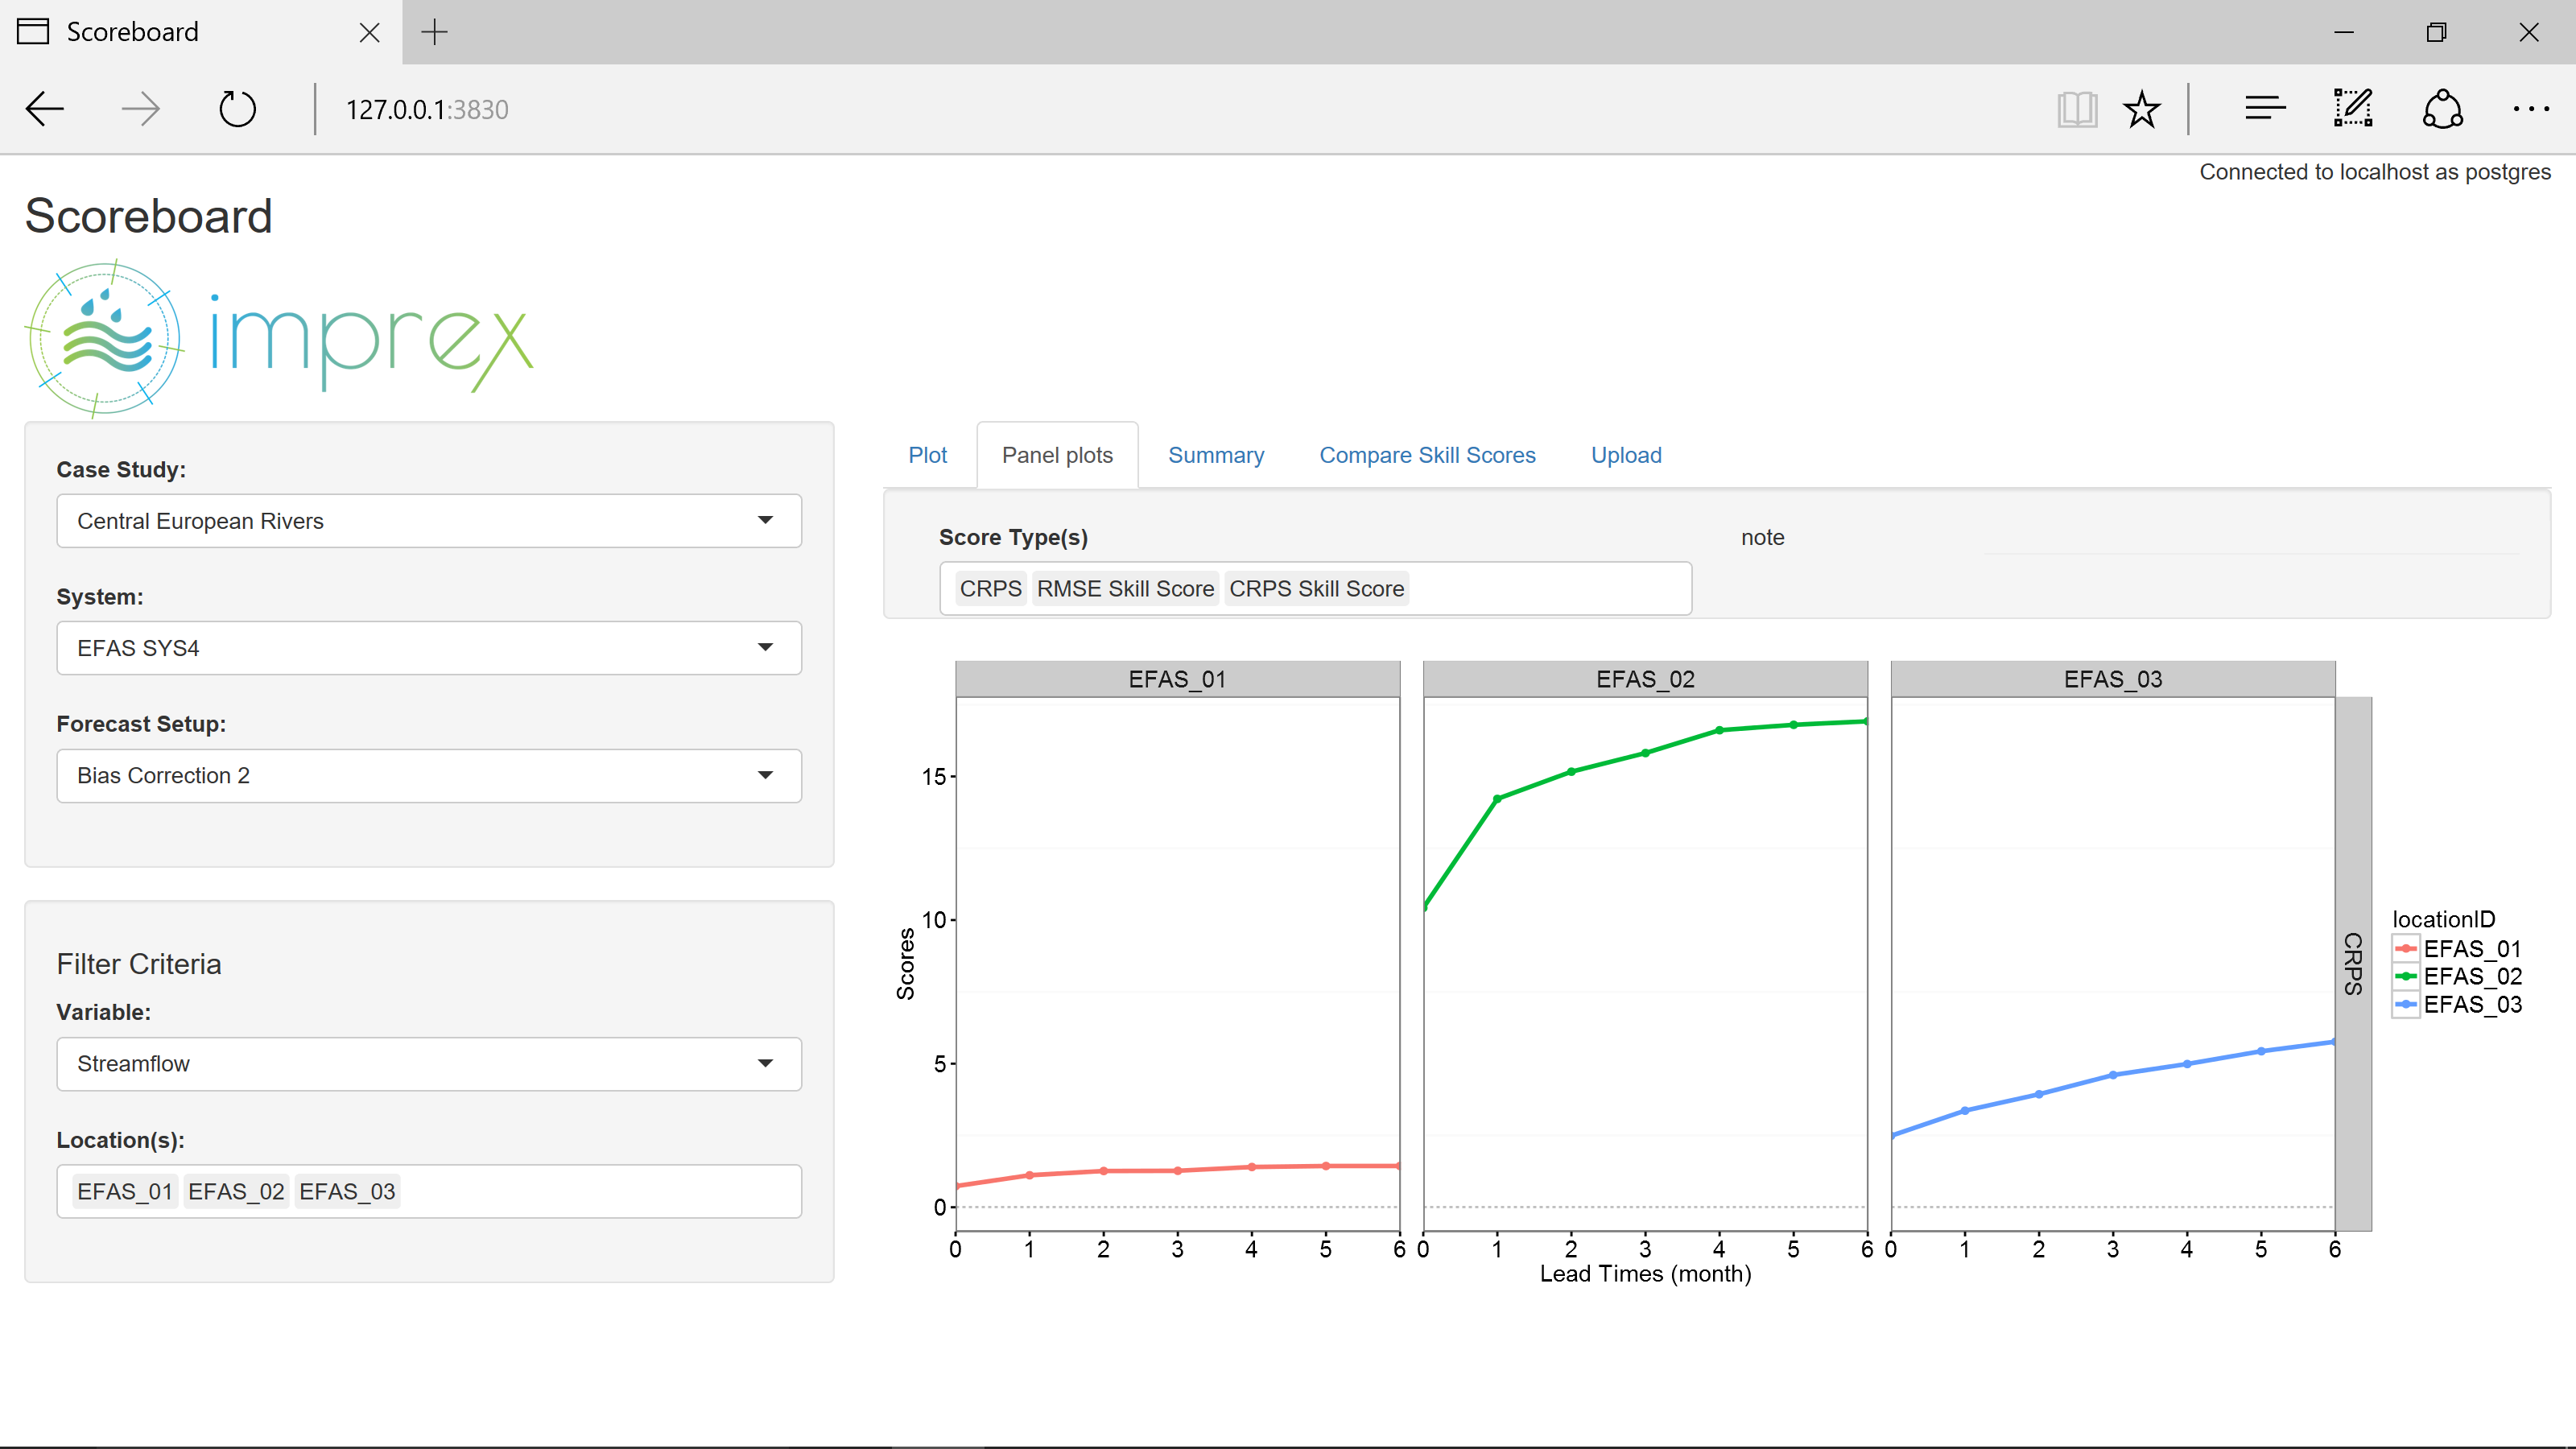
\includegraphics[width=0.85\linewidth]{images/isb2.png}
>>>>>>> 27270a97866f177710e5e08ee2c1f2f035a4f951
  \caption{Scoreboard Panel Plot function}
  \label{fig:isb2}
\end{figure}

Next, the ``Summary'' tab generates a small R-style summary of data currently selected. 

\begin{figure}[hb]
\centering
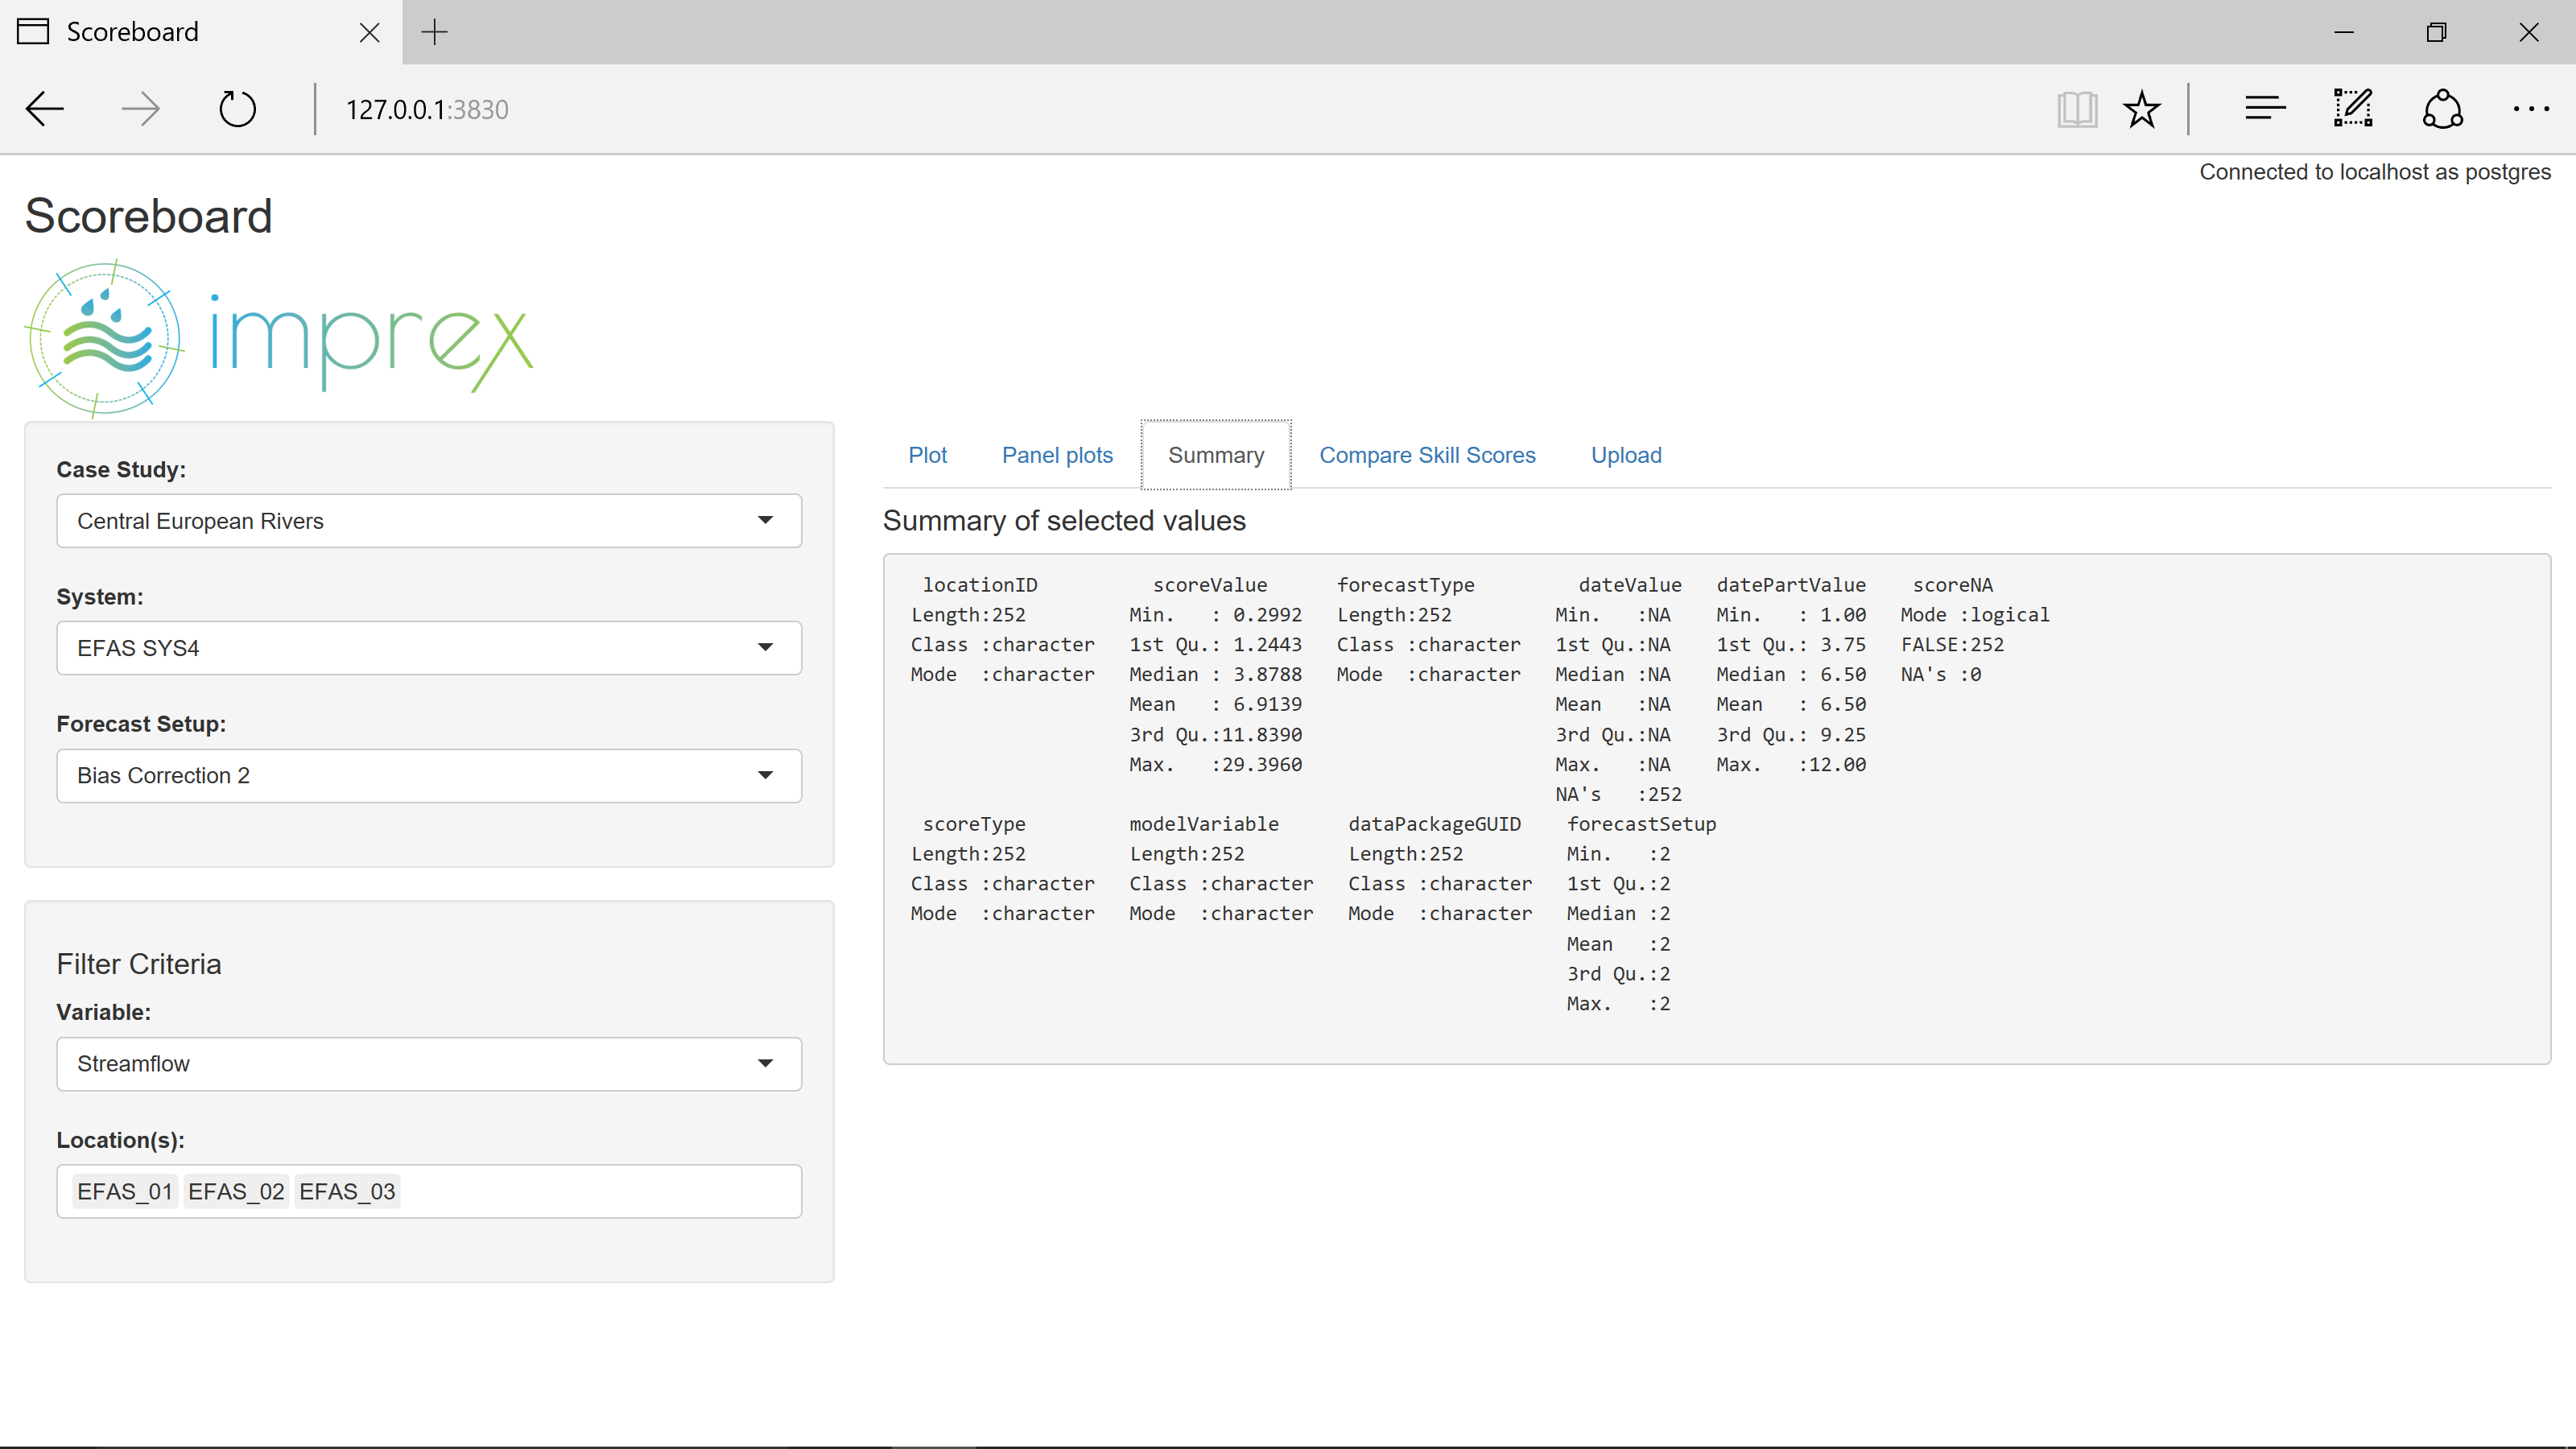
\includegraphics[width=0.80\linewidth]{images/isb3.png}
  \caption{Scoreboard Summary function}
  \label{fig:isb3}
\end{figure}

Finally, the tab titled ``Compare Skill Scores'' is next, and this allows the user to customize their own skill score.

\begin{figure}[H]
\centering
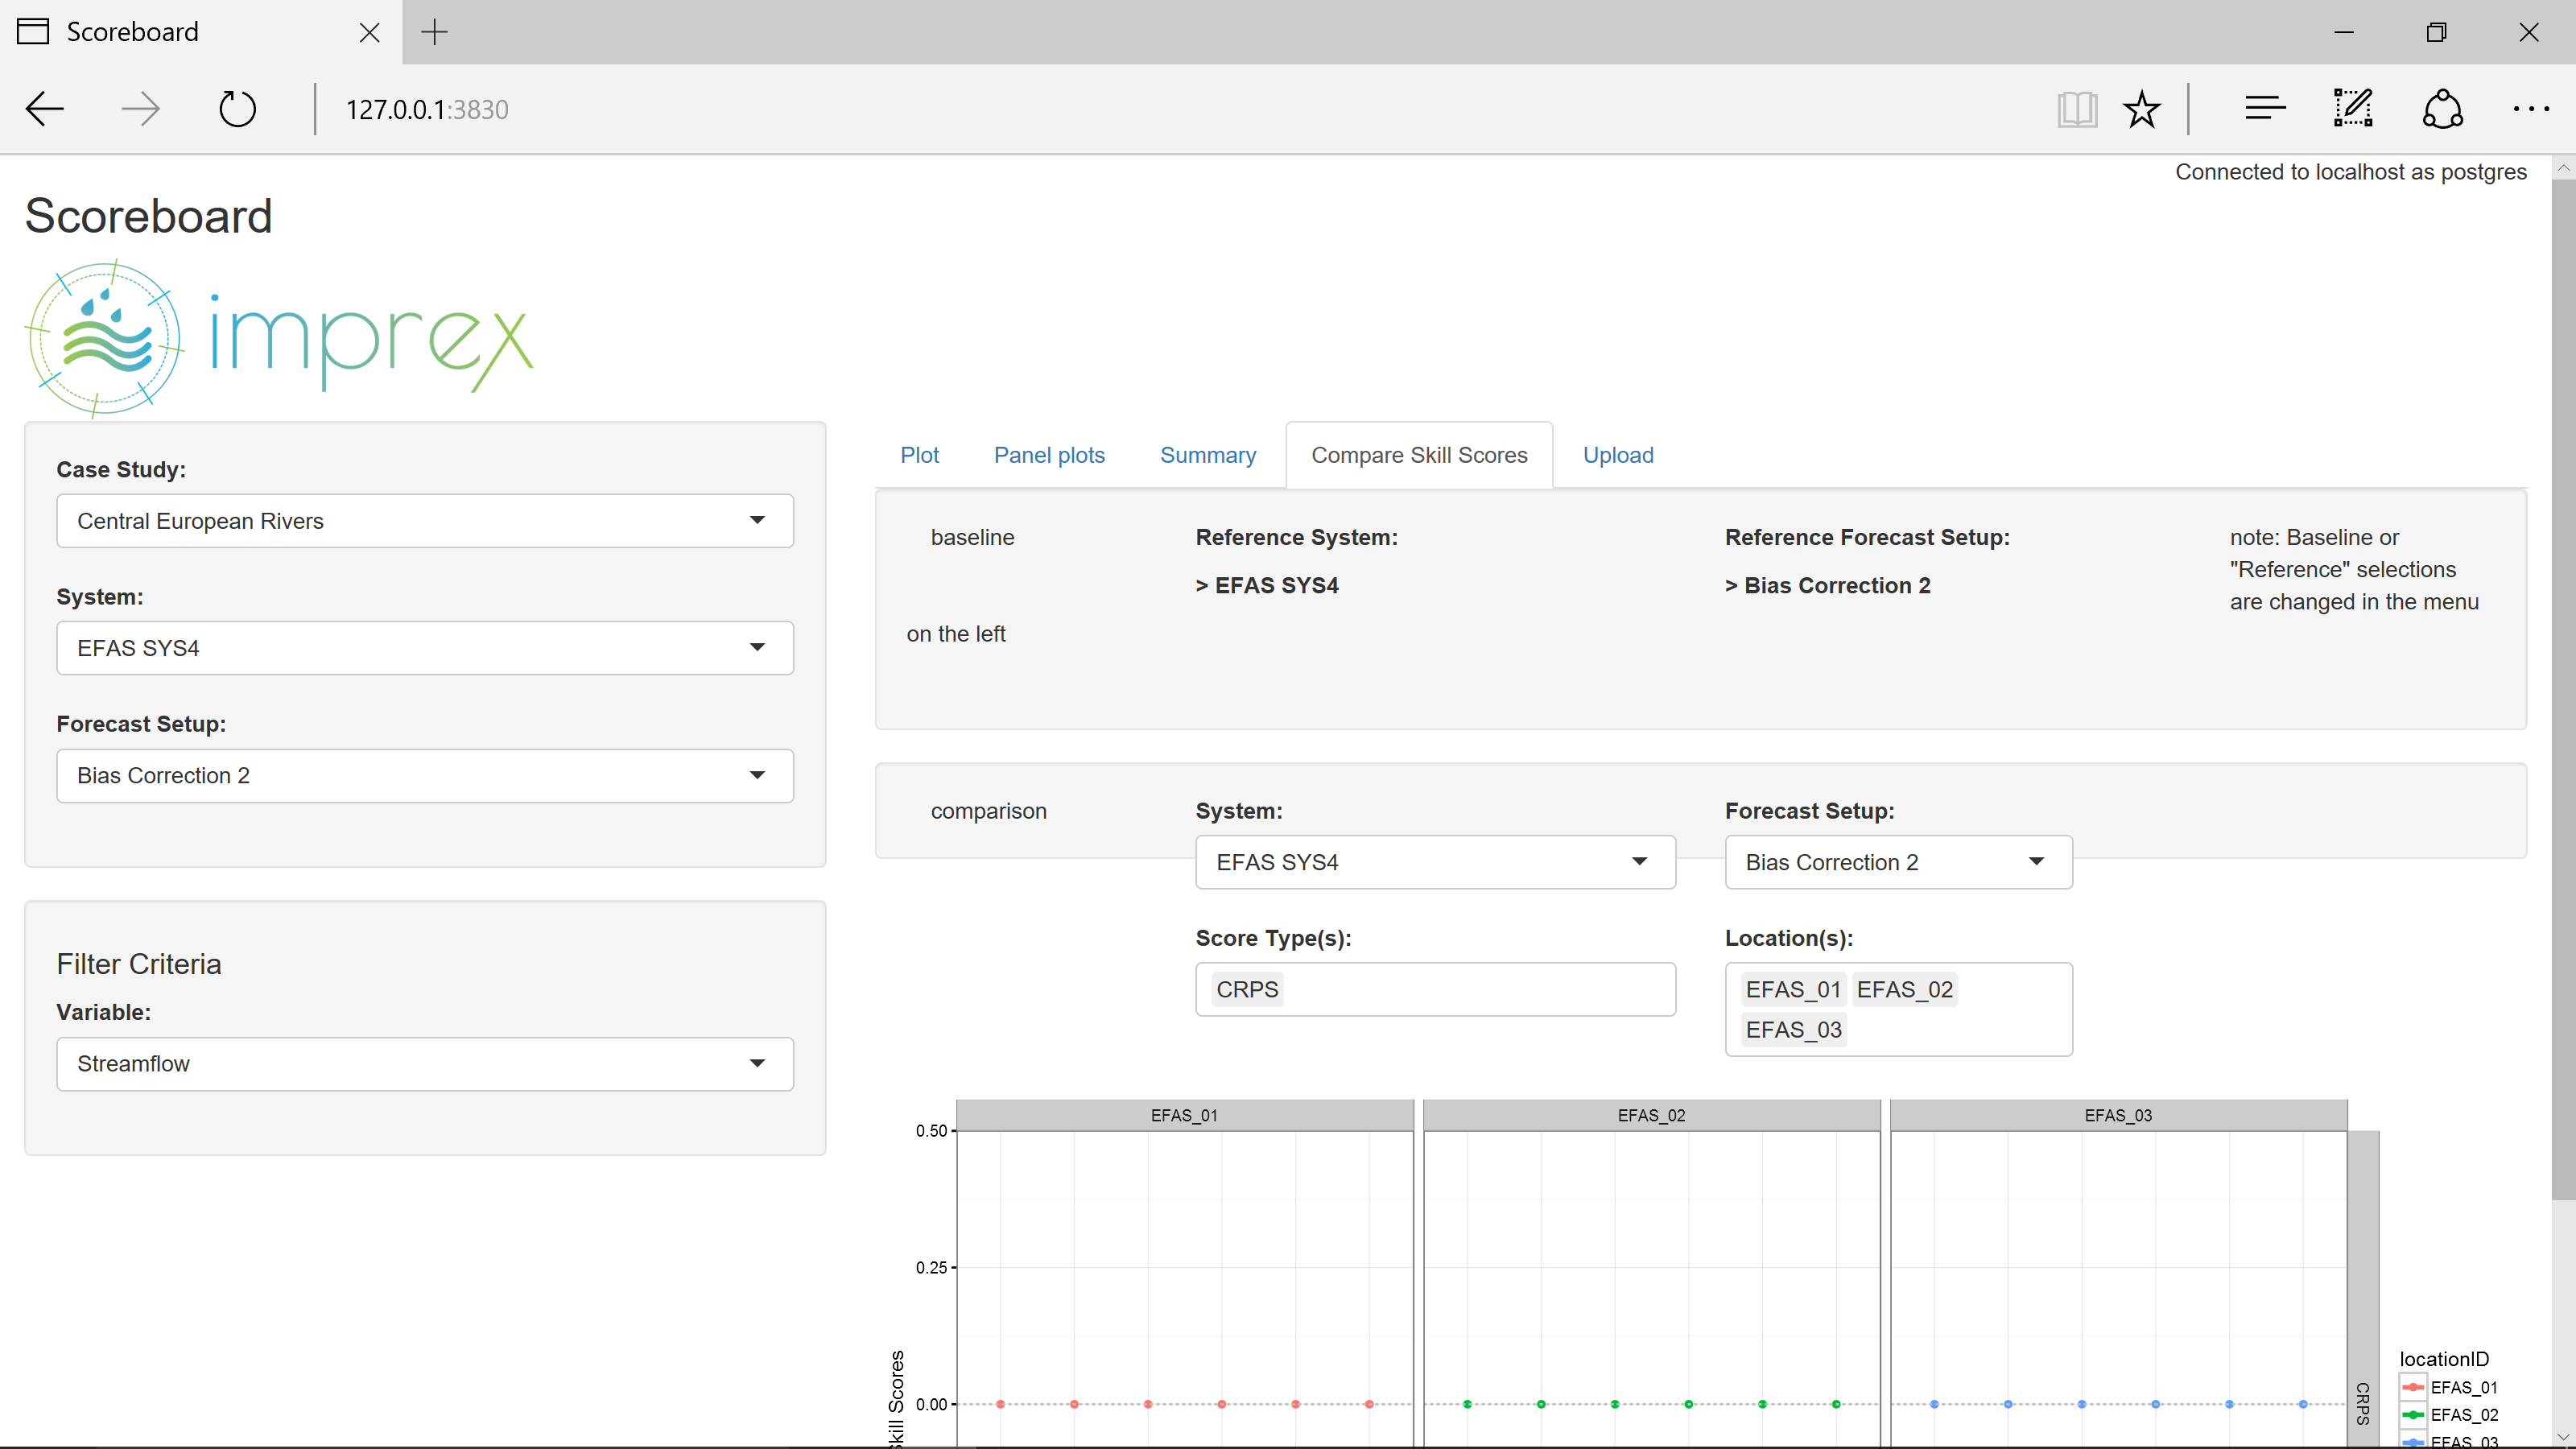
\includegraphics[width=0.80\linewidth]{images/isb4.png}
  \caption{Scoreboard Compare Skill Score Plots}
  \label{fig:isb4}
\end{figure}


The upper zone titled ``baseline'' mirrors the user's selections on the lefthand bar, in this case EFAS SYS4 and Bias Correction 2. This becomes the ``reference forecast''.

To make a comparison the user selects an available system under ``comparison''; it IS a valid choice to copy the ``baseline'' selections, but note that you are comparing the same System / Setup to itself; the plot will be zeros right across.

\begin{figure}[H]
\centering
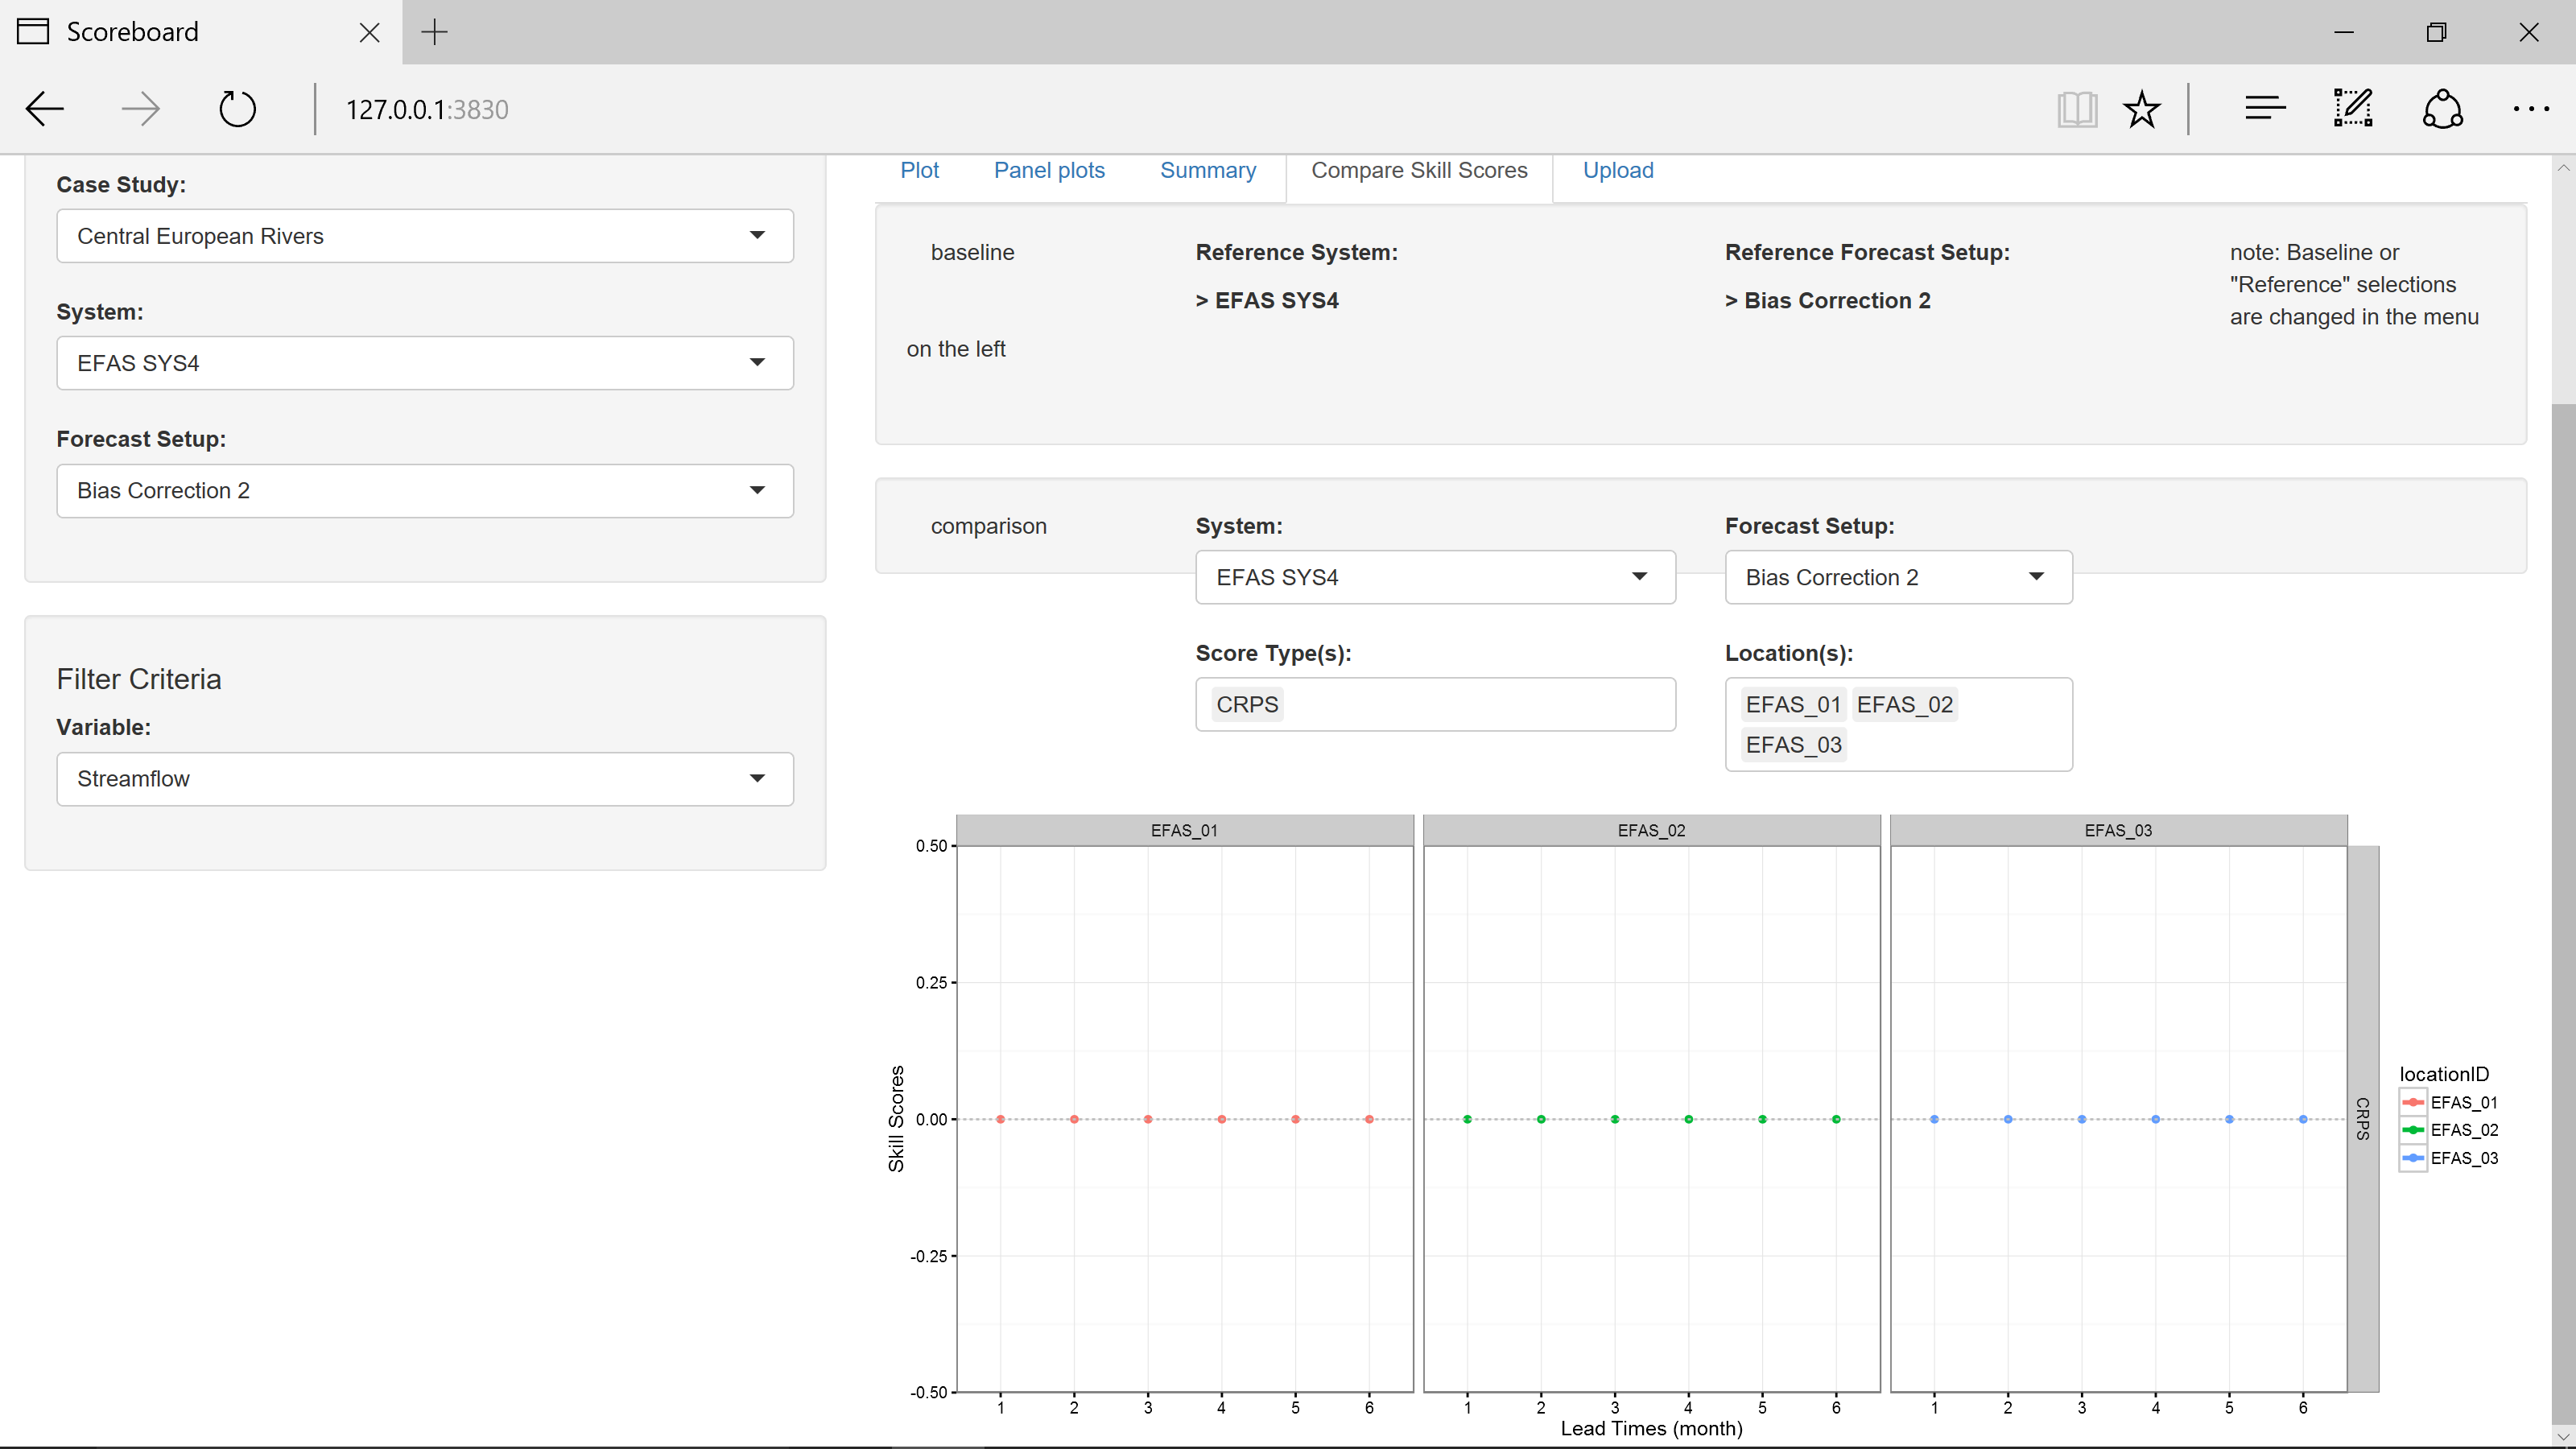
\includegraphics[width=0.85\linewidth]{images/isb5.png}
  \caption{Scoreboard Compare Skill Score Plots, lower part}
  \label{fig:isb5}
\end{figure}

If you chose a different System and Score, a new selection box becomes available: all possible Scores for that combination. On selecting a score (always CRPS for the test case), a new skill score plot will be made.


\begin{figure}[H]
\centering
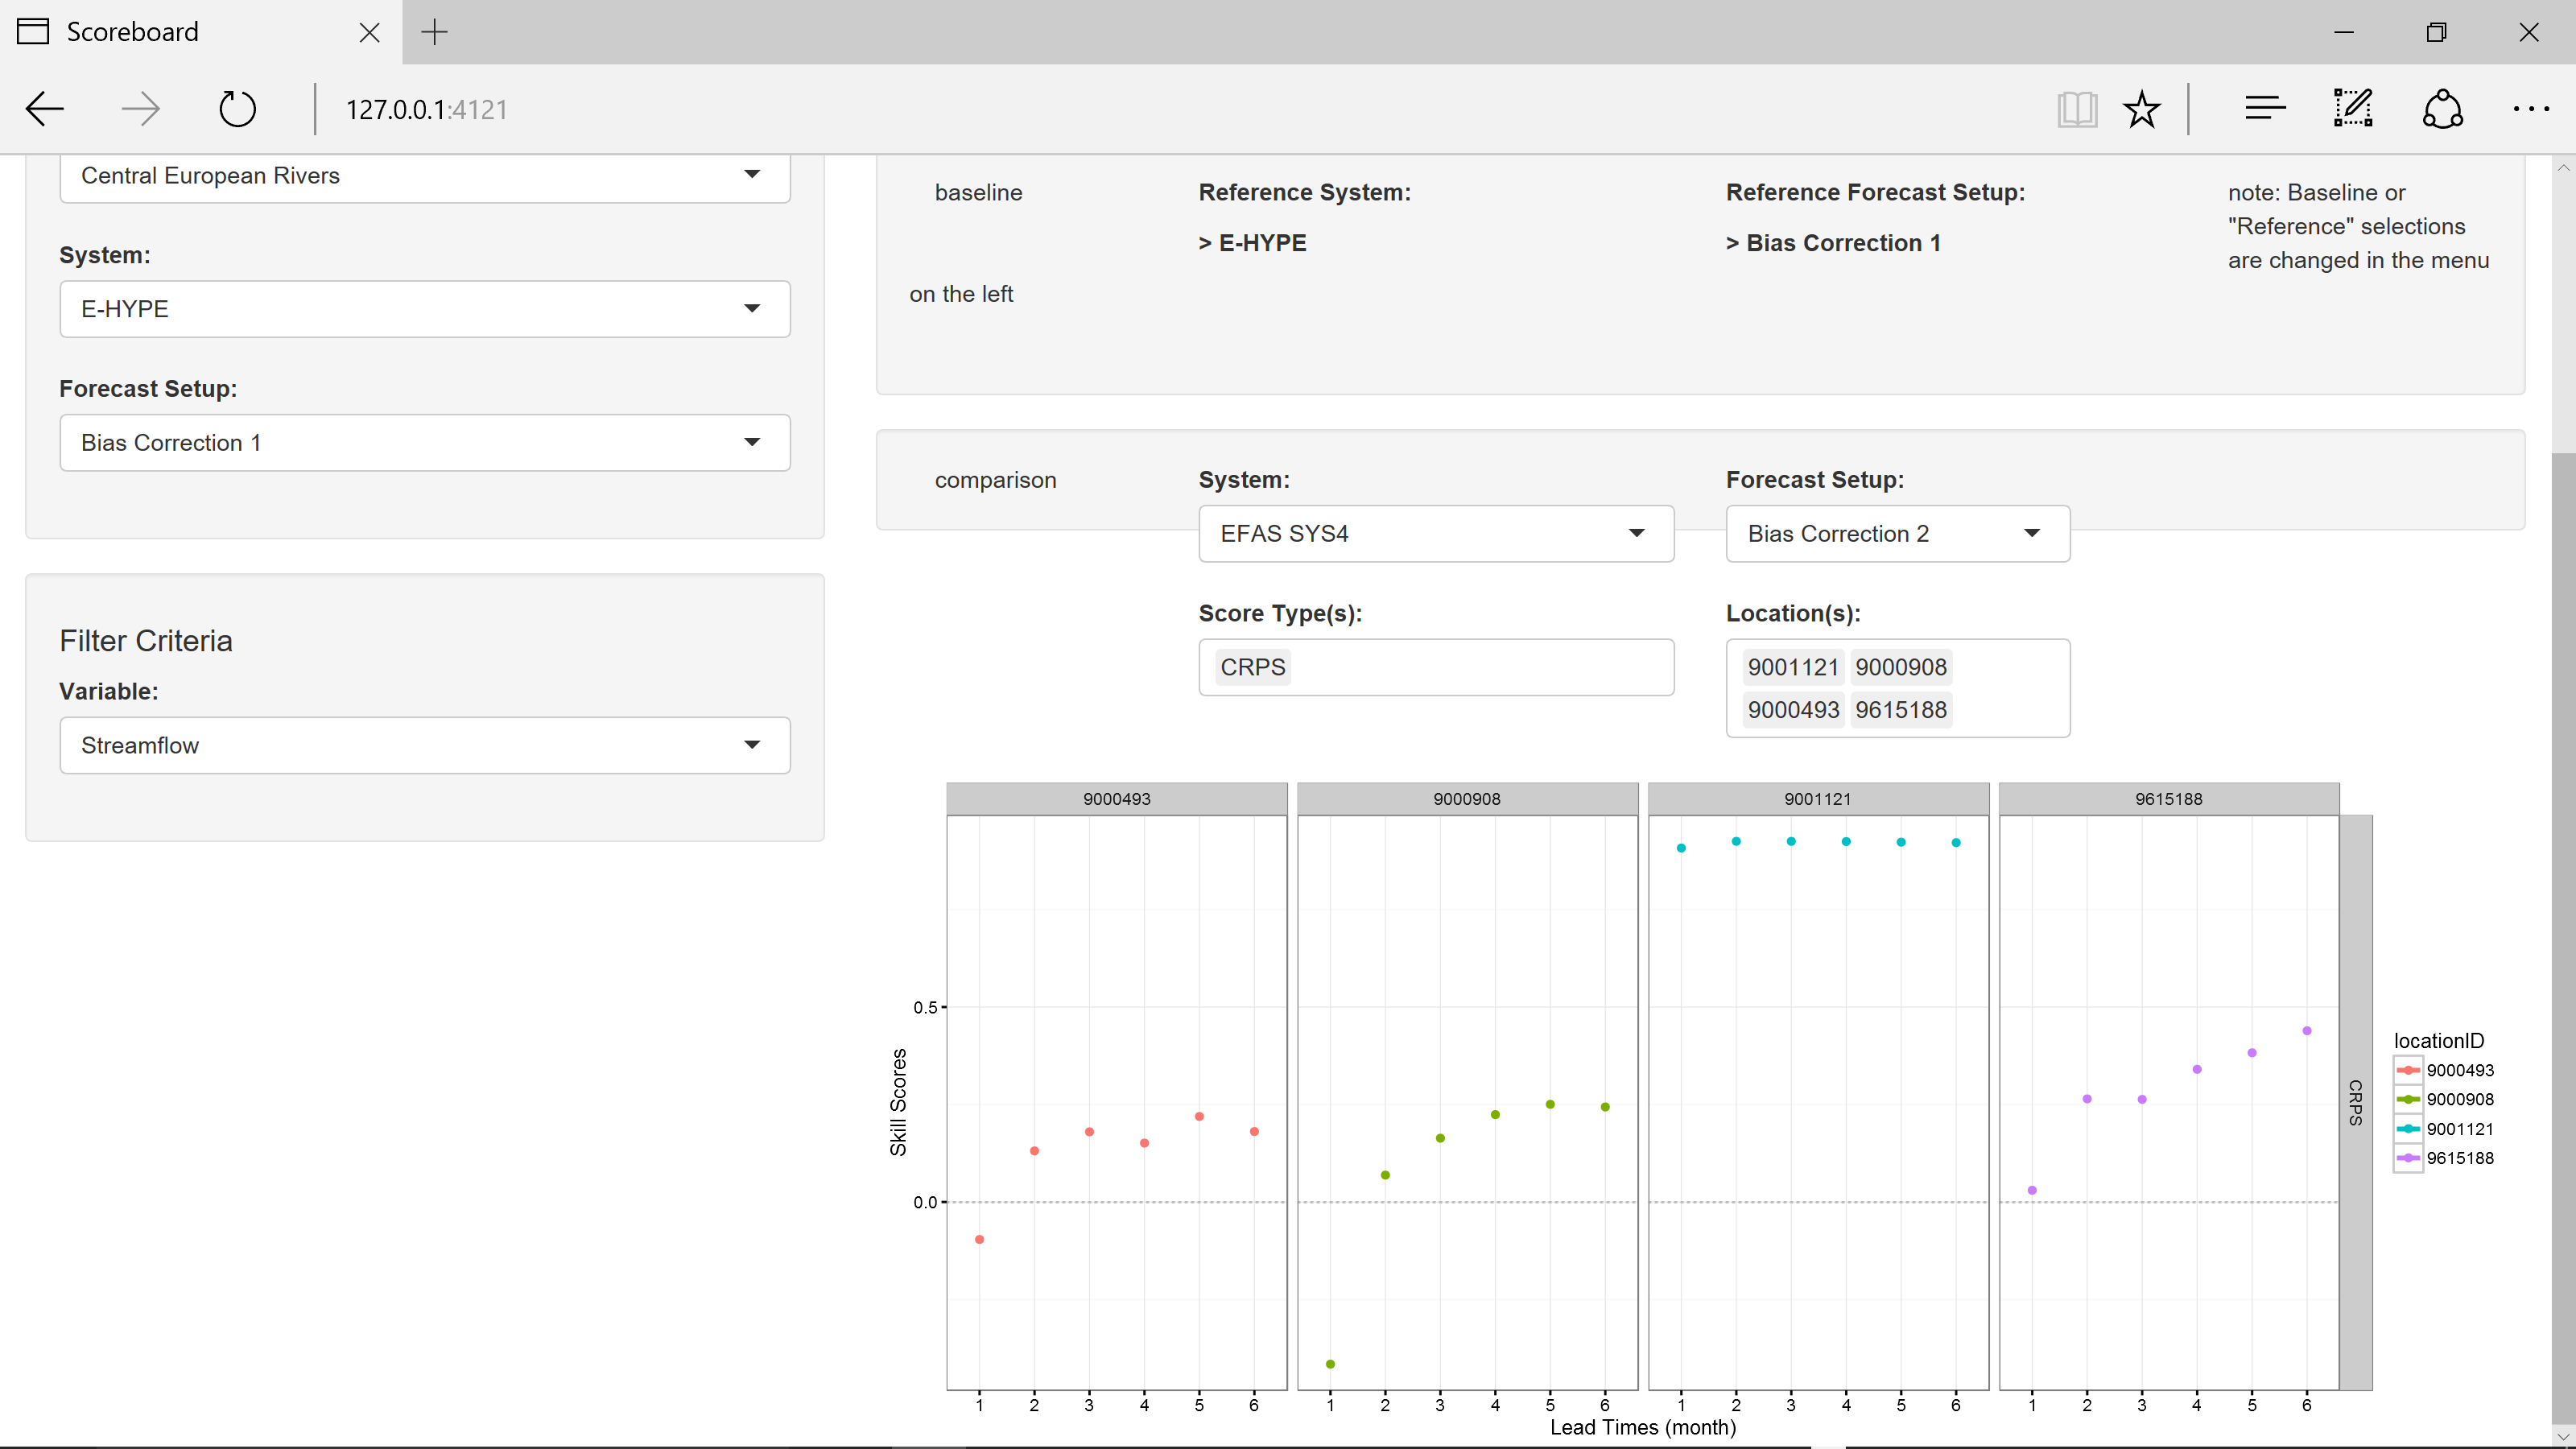
\includegraphics[width=0.85\linewidth]{images/isb5_2.png}
  \caption{Scoreboard Compare Skill Score Plots - Reference, Compare Forecasts shown}
  \label{fig:isb5_2}
\end{figure}

A value of zero (0) means the two forecast systems were perfectly aligned, or had identical skill. The other extreme on this scale is one, the maximum score; minus one (-1) is also valid, and the two indicated lack of skill. In the example here (Figure \ref{fig:isb5_2}), the reference system is E-HYPE; it's being compared with EFAS SYS4. The first plot (9000493) shows that at a lead time 1 EHYPE does a bit better than EFAS; however, from LT = 2 through 6 EHYPE loses while EFAS manages increasing lead times better.

That is generally repeated with 9000908 and 9615188. Location 9001121 shows EFAS consistently better.


\begin{figure}[h]
\centering
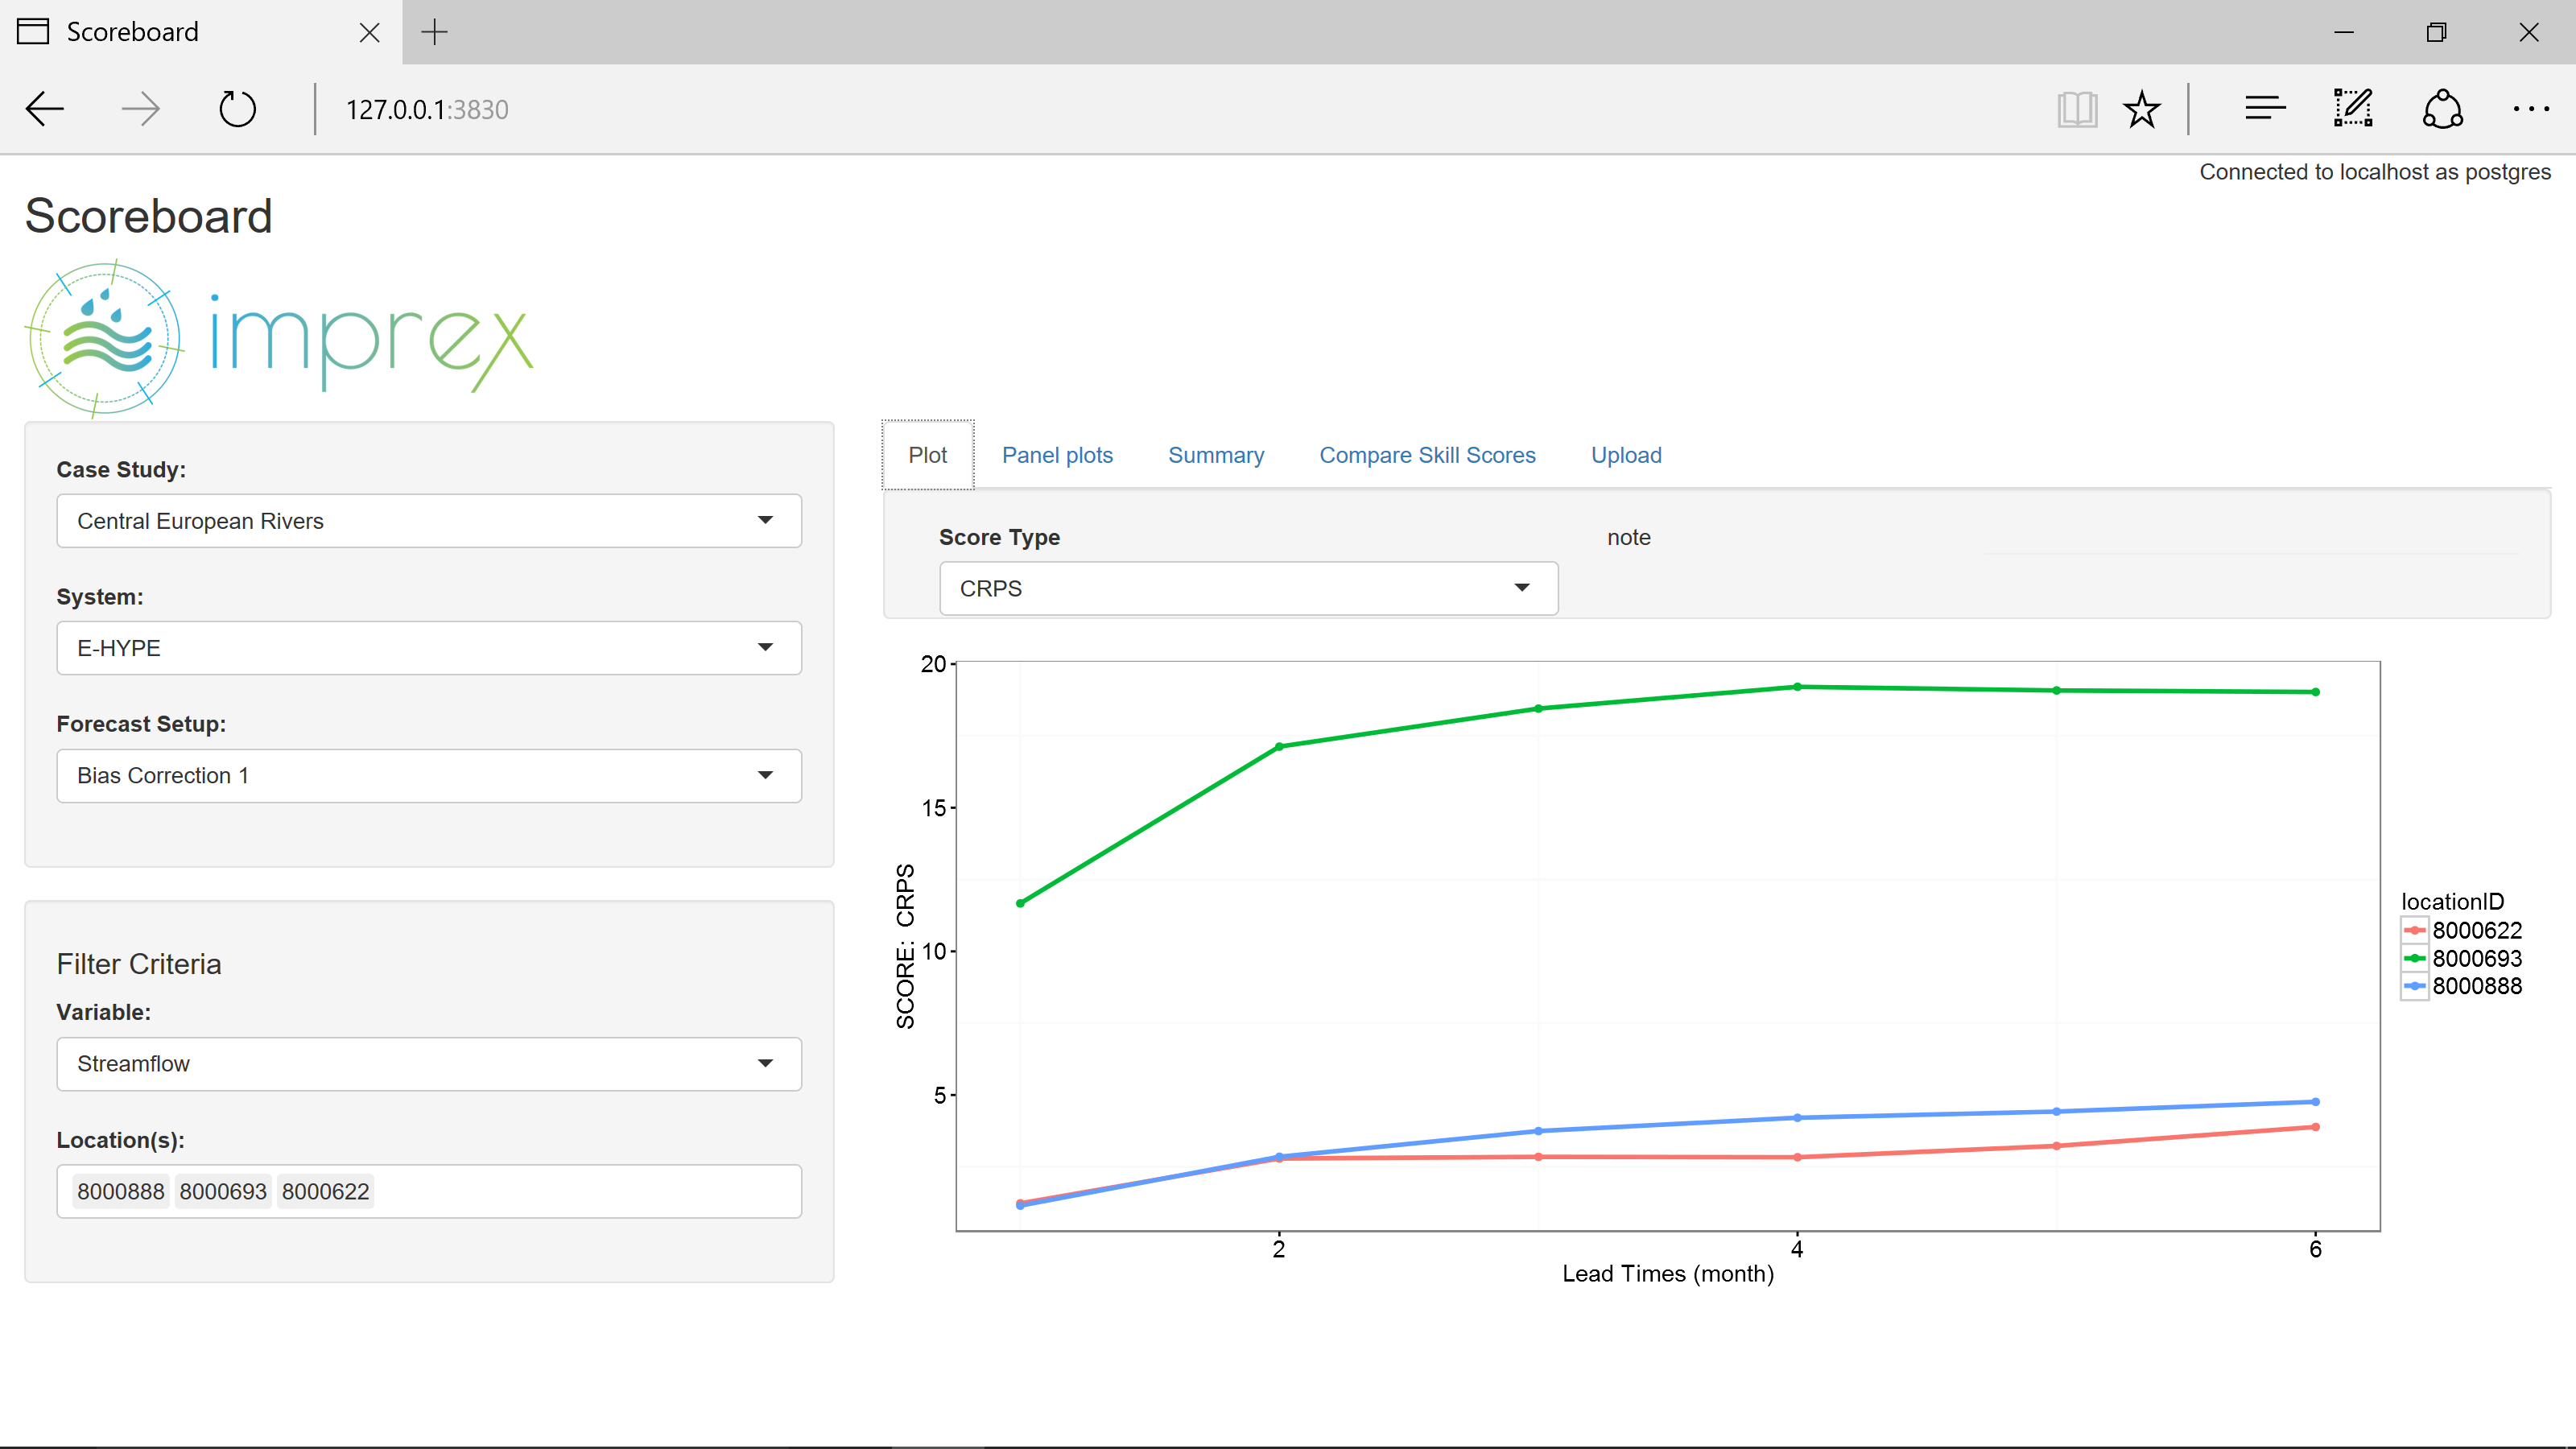
\includegraphics[width=0.80\linewidth]{images/isb6.png}
  \caption{Scoreboard Plot - changed System, Setup automatically adjusts}
  \label{fig:isb6}
\end{figure}

\begin{figure}[h]
\centering
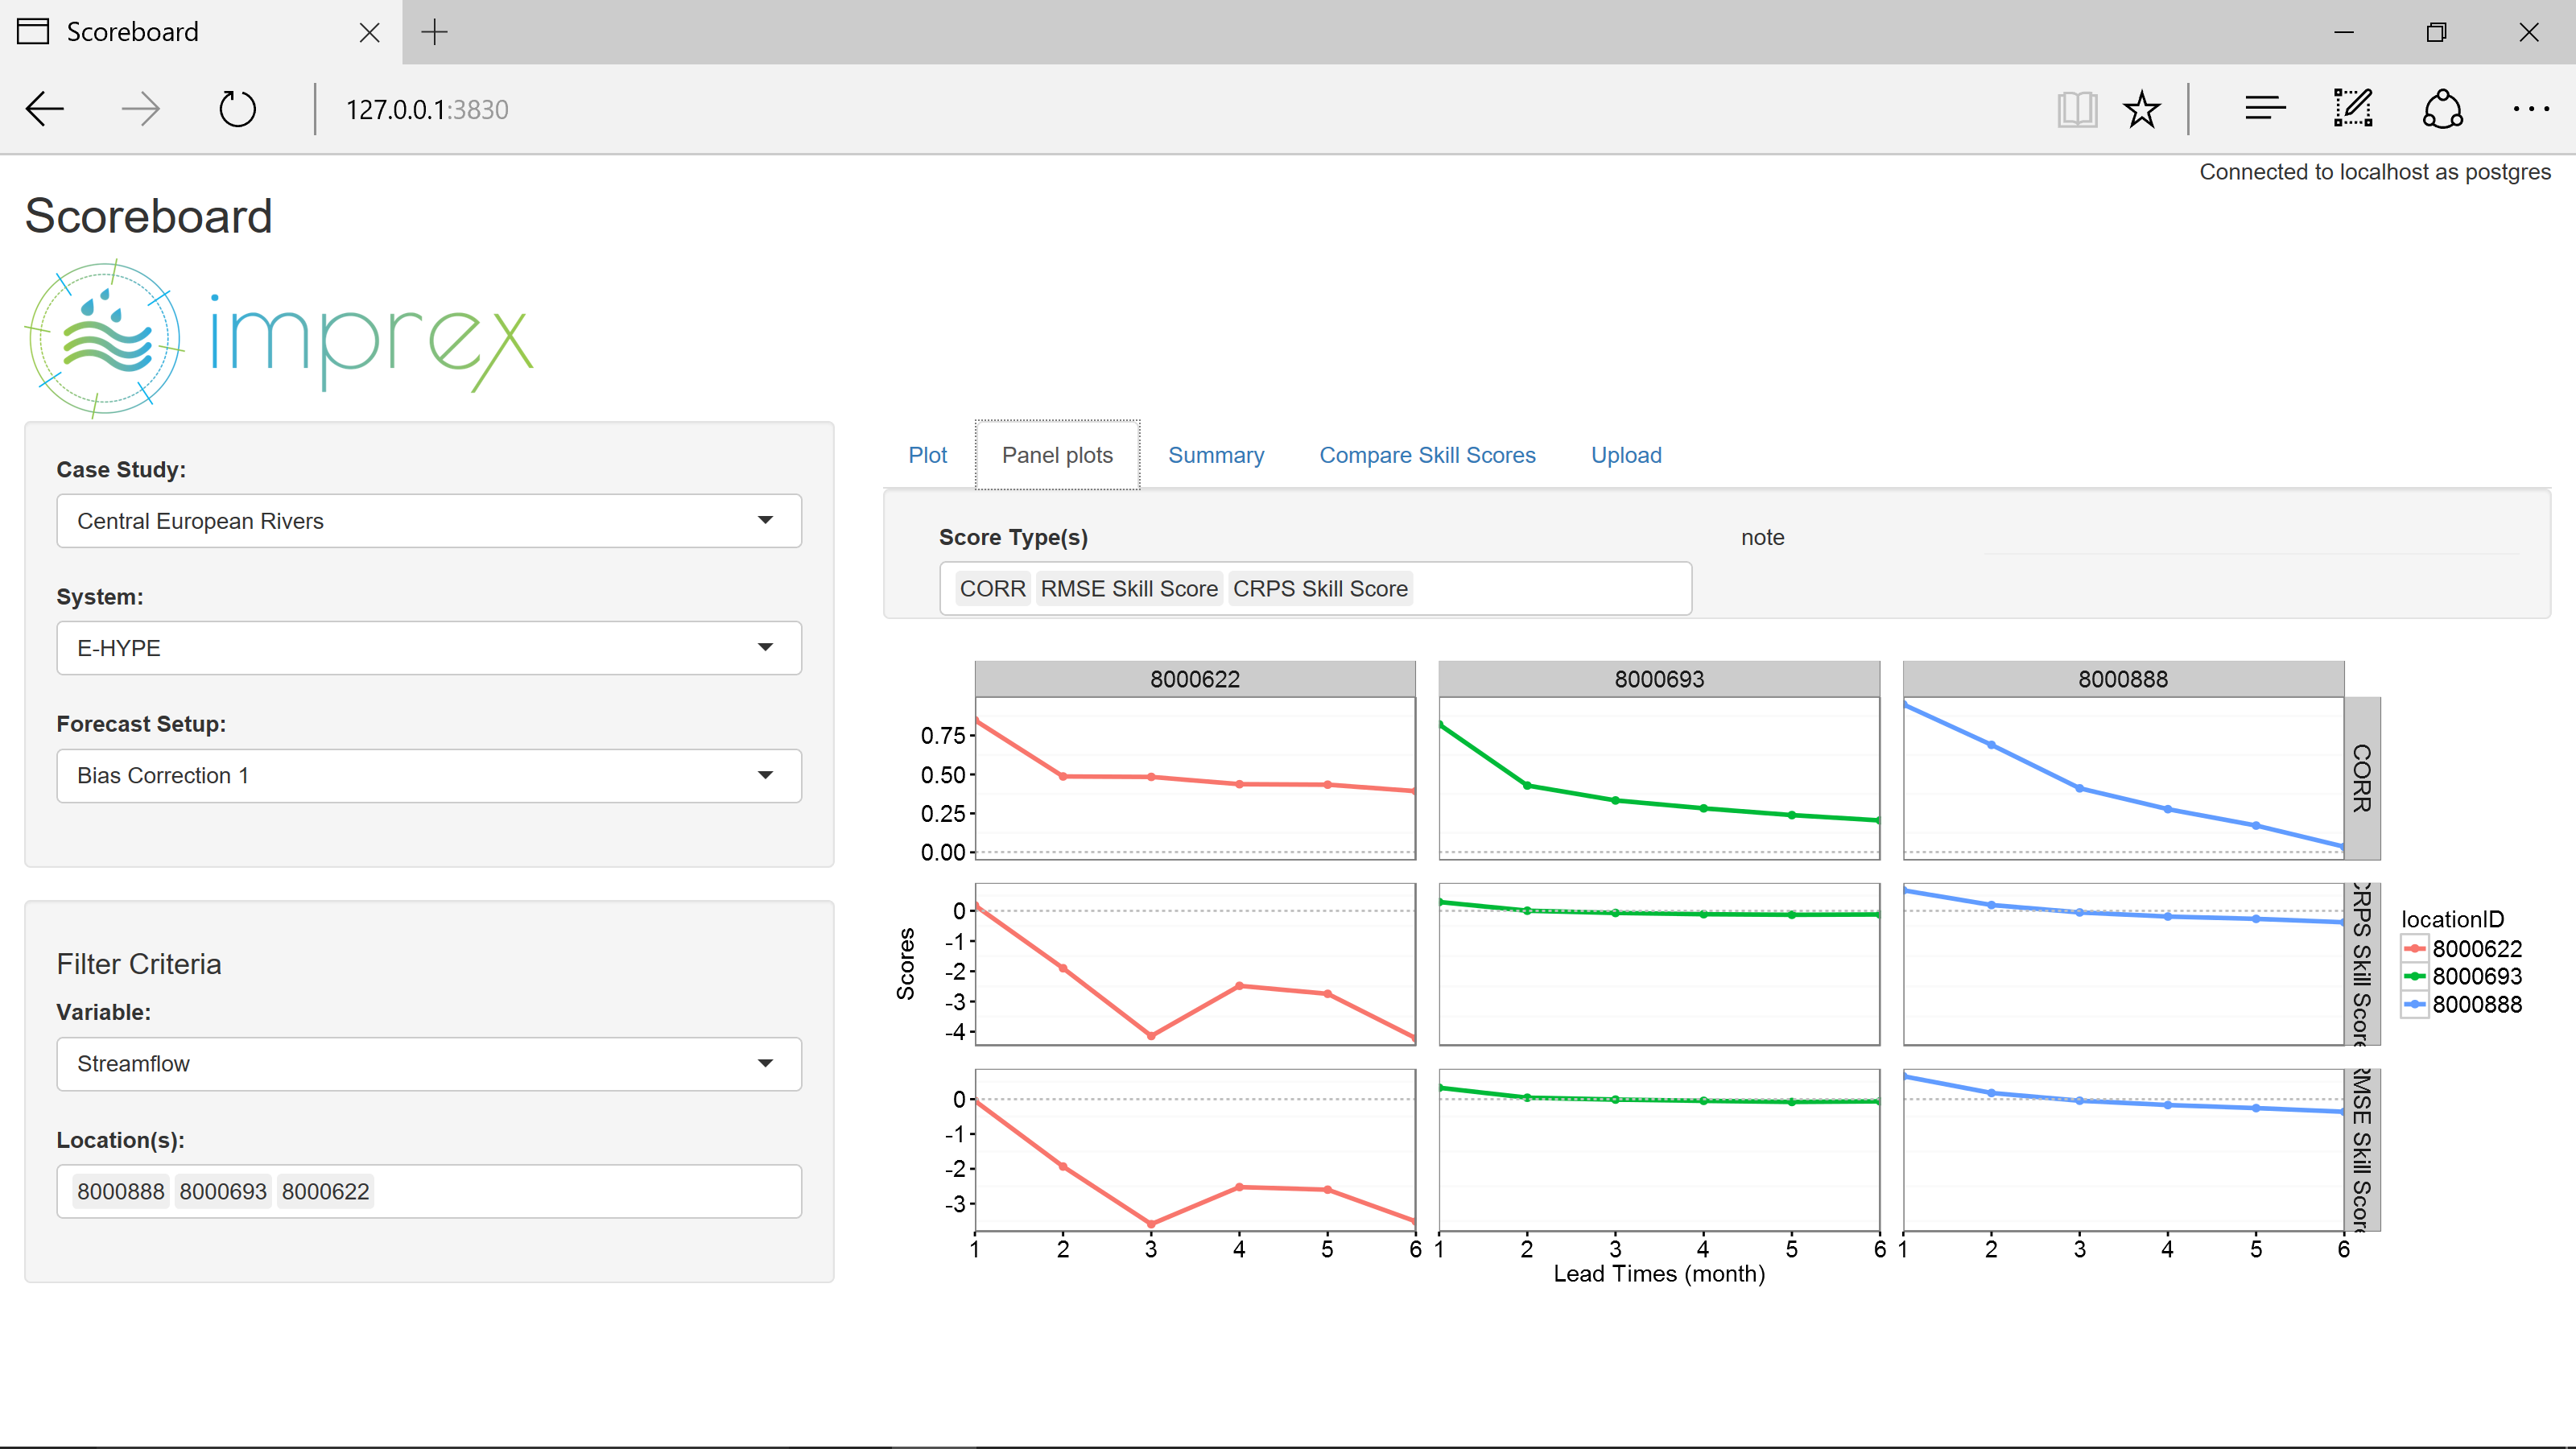
\includegraphics[width=0.80\linewidth]{images/isb7.png}
  \caption{Scoreboard Panel Plots}
  \label{fig:isb7}
\end{figure}

%\section{Assigning Reference Forecast}
%\section{Loading a New Dataset}

%\begin{figure}[hp]
%\centering
%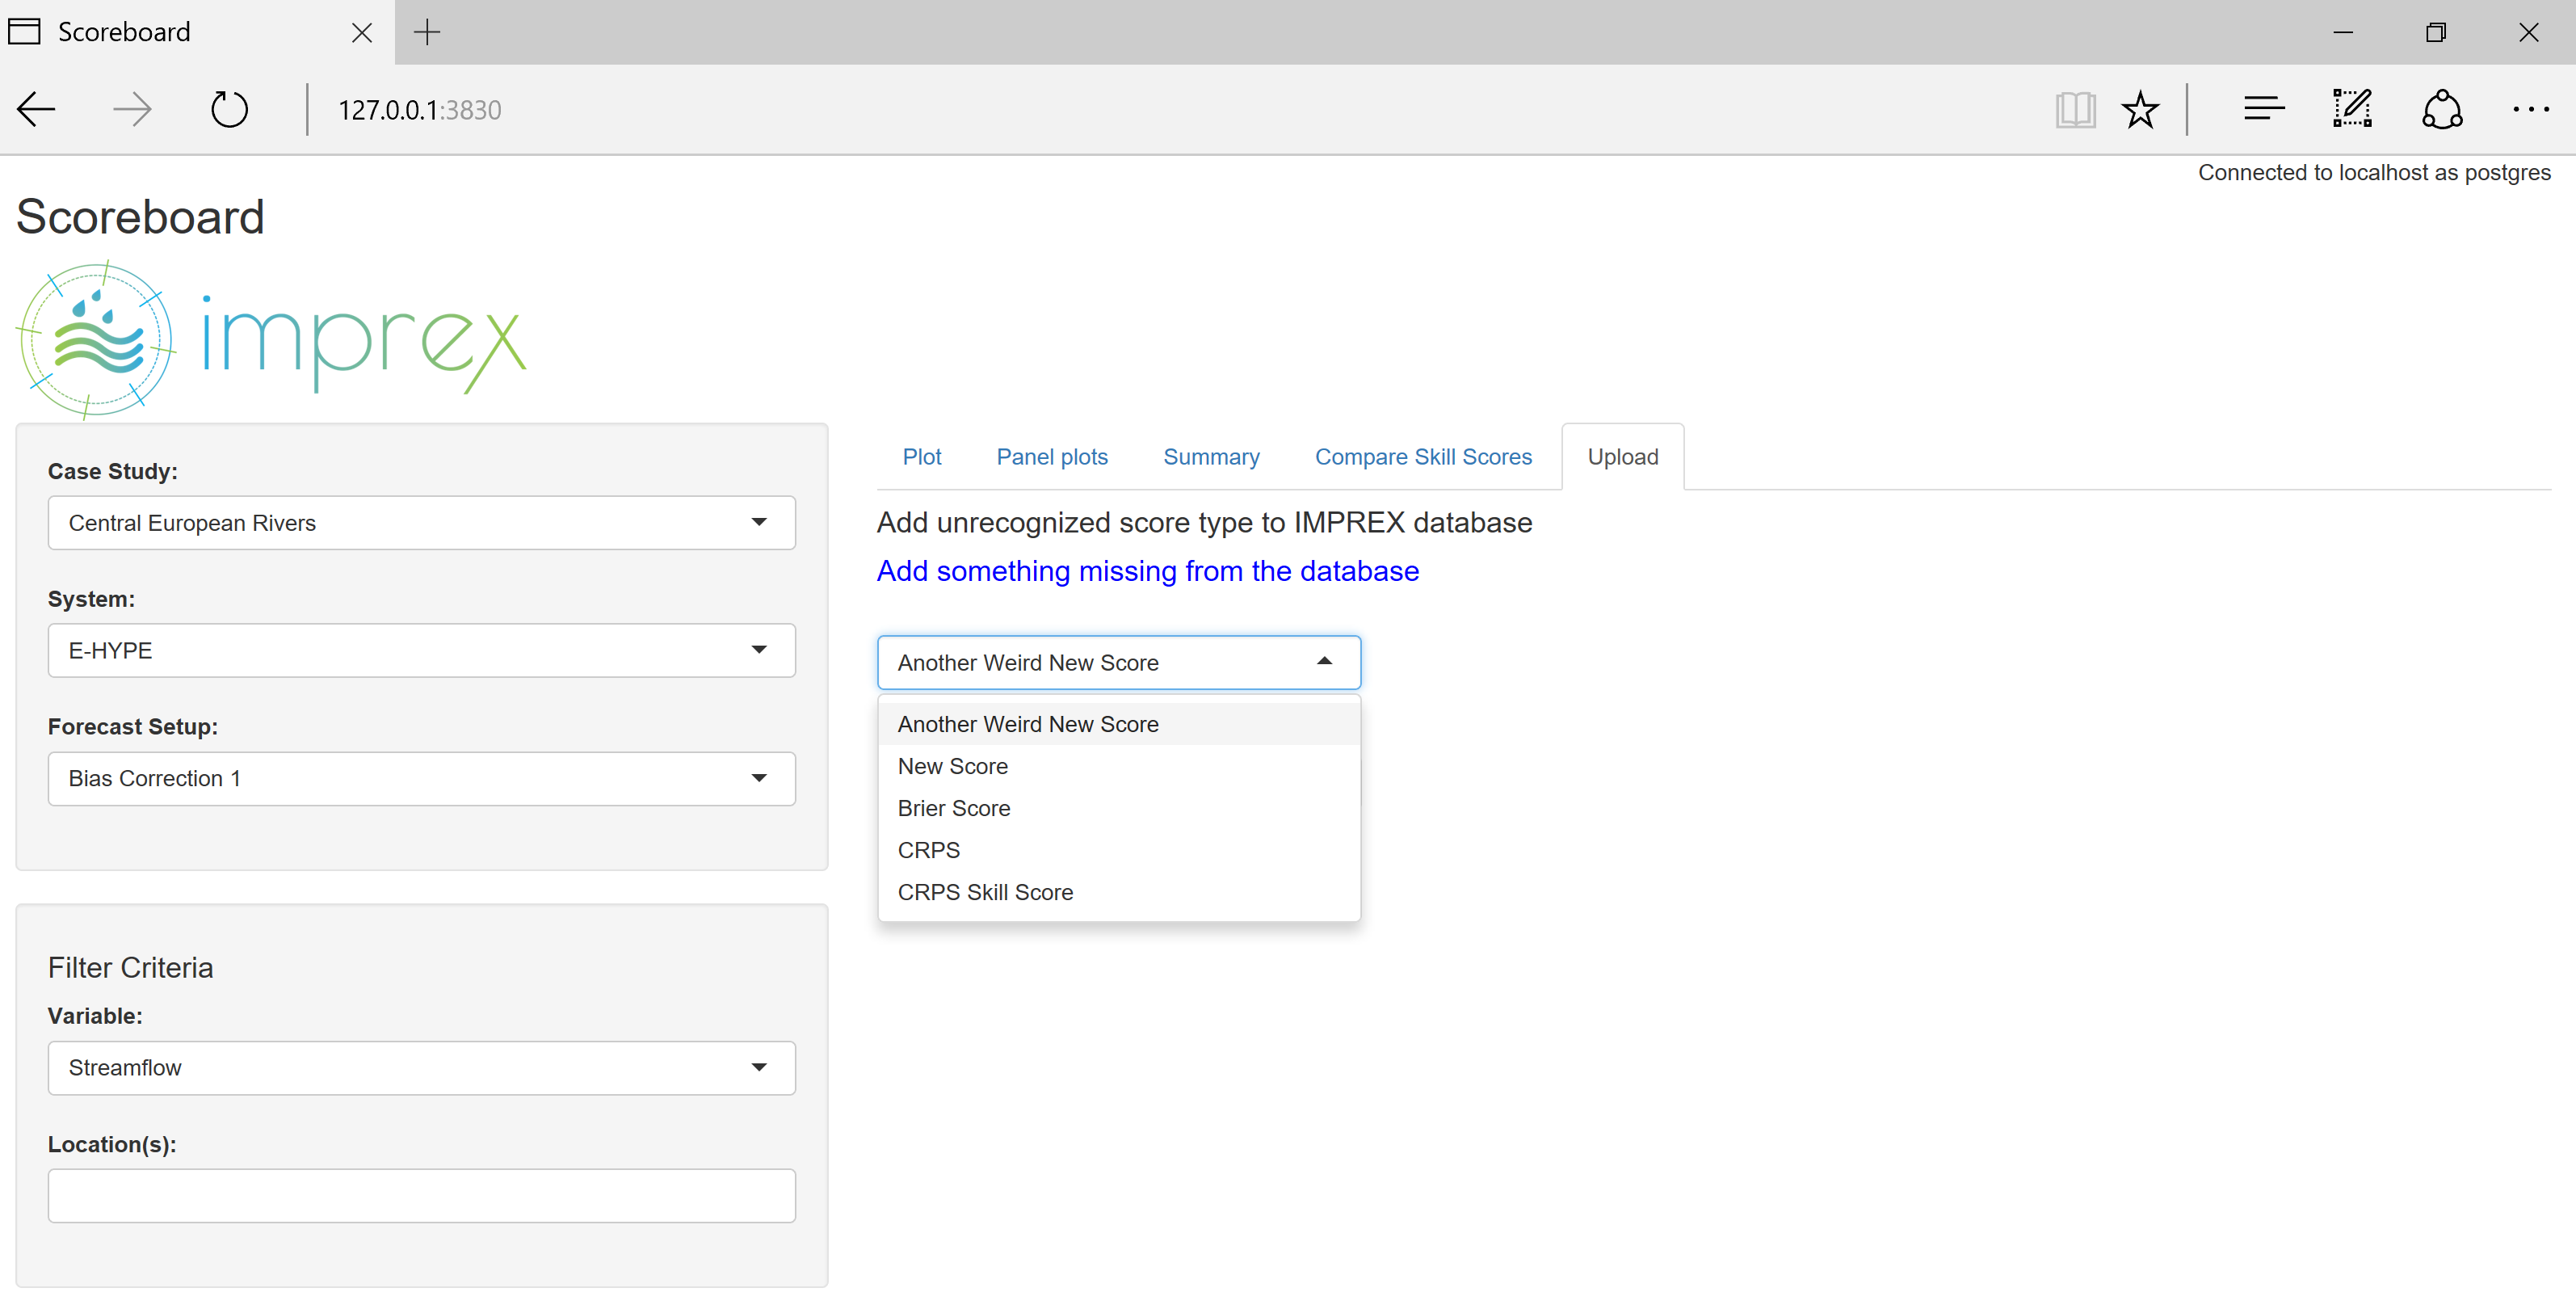
\includegraphics[width=0.90\linewidth]{images/imprexUpload1.png}
%  \caption{Database Interface to Upload and Add New Scores}
%  \label{fig:imprexUpload}
%\end{figure}
%


\subsection{Conclusion on the Design of the Scoreboard}

In order to evaluate scoreboard performance and features we evaluated the scoreboard installed on one computer. At the time of testing we did not use remote servers for the database nor the web pages.

Overall the scoreboard meets our design goals, and provides three graphical plotting interfaces: Plot, Panel Plot, and Compare Skill Scores. The user can navigate between the interfaces, changing criteria and exploring how models diverge in skill over time and according to different forecast setups (ex Bias Correction, post processing, etc).

As we tested on one local computer, moving the system to a hosted solution (PostgreSQL server, Shiny server) infrastructure may increase latency within the application. If this is the case, adding a ``progress bar'' to let the user know when a slow query is taking place may improve responses to the interface. Additional tuning of the software may be investigated.

% \subsection{Examples}

\strut\newpage

%########################################################################
% Annexes / Appendices
%########################################################################

\part{General Conclusions and Way Forward}

Forecasting hydrology and meteorology events involves complex systems of data collection, physical and/or empirical modeling. This project targeted only an understanding of the verification process -- evaluating predicted values against an observation or confident value -- and the numerical scores that modelers may produce. Finally, the project succeeded in defined and constructing a useful and interesting utility that had not existed before.

There are clear opportunities to improve the scoreboard as it exists today. The reporting system (outputting graphics and PDF files of queries created) is not complete, as the creators of Shiny have change their libraries; a more robust system of saving markdown PDFs is available. Our upload system works on well-formatted RDS files, but is inflexible about reporting errors.

As noted in the report, currently we select a ``location'' from a list; with increasing numbers of users, both data submitters and evaluaters, the location identifiers will become impossible to evaluate. Implementing a graphical system for point selection is important. 

Finally, with increasing numbers of users we will begin hearing more community feedback, and ideas from those with expertise in forecast verification -- and a little distance from the tool itself -- for improvements and changes.



%########################################################################
% Bibliography
%########################################################################
\thispagestyle{empty}
\strut\newpage

% \addcontentsline{toc}{subsection}{References} %\\moves text right
\addcontentsline{toc}{section}{References}
%\section{References}

\begin{thebibliography}{100}
	\labelwidth=4em
	\addtolength\leftskip{25pt}
	\setlength\labelsep{0pt}
	\addtolength\parskip{\smallskipamount}
\printbibliography 

\end{thebibliography}

%########################################################################
% Document end
%########################################################################

\end{document}
